%!TEX root = ../main.tex

%il faut decrire la structure de notre chapitre 
For the analysis of our algorithms and data structures, we decided to analyze the run time on three types of instances :
\begin{description}
\item[Density variation instance :]{Graphs having a fixed number of vertices ($|V|=1000$) and a density of edges ranging from 5 to 100\%. The maximum capacity of an edge is 10000.}
\item[Size variation instances :]{Graphs having a density of edges fixed (10\%) and a number of vertices varying from $|V|=1000$ to $|V|=5000$. The maximum capacity of an edge is 10000.}
\item[Matching instances :]{Graphs having a source $s$, a destination $t$ and two groups of 500 edges $R1$ and $R2$. 500 edges connect $s$ to all vertices in $R1$ and 500 other edges connect all vertices in $R2$ to $t$. All other possible edges can only go from $R1$ to $R2$. The graphs have a density of $R1$->$R2$ edges ranging from 5 to 100\%. The capacity of all edges is 1.

The Figure~\ref{fig:matching} represents a matching instance with a density of $R1$->$R2$ edges equal to 100\%.

\begin{figure}[H]
\begin{center}
\includegraphics[scale=0.3]{images/matchinginstance.png}
\caption{Matching instance with a density of edges equal to 100\%.}
\label{fig:matching}
\end{center}
\end{figure}}
\end{description} 

\section{Instances generation}
To obtain the necessary instances, we implement instances generators which respects the characteristics of the network graphs (a connected graph where each vertex has at least one incoming and one outgoing edge).

\subsection{Density variation instances}
For the density variation instances, we first create a minimal connected graph. To do this, let $Connected$ be the set of the connected vertices, $DoubleConnected$ the set of vertex having at least one incoming and one outgoing edge, $Edges$ the set of edges and $AllEdges$ the set of all possible edges. Initially, $Connected$ contains the vertex 0, $DoubleConnected$ and $Edges$ are empty and $AllEdges$ contains all possible edges. When we want to add a vertex $v$ to the graph, we take a random vertex $r$ from $Connected$, add the edge ($v$,$r$) in $Edges$, add $v$ in $Connected$, remove the edges ($v$,$r$) and ($r$,$v$) from $AllEdges$ and add $r$ in $DoubleConnected$. After adding our 1000 vertices, we have a connected graph where each vertex has one incoming edge and sometimes at least one outgoing edge (all vertices in $DoubleConnected$).

For each vertex not present in $DoubleConnected$, we take a random vertex from $Connected$, add the edge between them in $Edges$ and remove this edge and its opposite from $AllEdges$. For this step, to avoid adding an edge (or its opposite) which is already present in the graph, we check if the new edge and its opposite are not present in $Edges$. We thus have a connected graph where each vertex has one incoming edge and at least one outgoing edge.

We then add the necessary number of edges to obtain the desired density. We take a random edge from $AllEdges$, add it to $Edges$ and remove it and its opposite from $AllEdges$. A first graph is generated when we have a density of 5\%. We add it edges to obtain a density of 10\% and generate a second graph. And so on up to 100\%. At the end, a density variation instance is composed by twenty graphs where each graph generated before an other one is a sub-graph of the latter.

With $|V|=1000$, a complete graph has $\frac{(|V|-1)(|V|)}{2} = 499500$ edges.

We generate 10 instances of this type.

\subsection{Size variation instances}
For the size variation instances, we use the same technique as for the density variation instances without the $AllEdges$ set. Indeed, it is not necessary to generate all possible edges for graphs with a 10\% of edge density. Especially when we know that a complete graph with $|V|=5000$ has 12497500 edges. To know if an edge (or its opposite) is already present in the graph, we check if it is contained in $Edges$.

We generate a network graph with $|V|=1000$ and an edge density of 10\%. We add it 500 vertices and the corresponding edges to respect the characteristics of the network graphs. We add then the necessary edges to keep a 10\% edge density and generate this new graph. And so on until $|V|=5000$. At the end, a size variation instance is composed by nine graphs where each graph generated before an other one is a sub-graph of the latter.

We generate 10 instances of this type.

%Pour cette section, j'ai mis des noms comme ça mais fait toi plaiz si tu trouves des noms plus appropriés :).
\section{Push-Relabel}
In this section, we will analyze how the different heuristics performs in the push-relabel algorithm. We also tried each heuristic with and without the height label initialization phase (as explained in Chapter~\ref{improvements}) to show if this phase is useful in practice.
\subsection{Height label initialization}

To analyze the effects of the height label initialization, we decided to compute the number of operations performed. In the preflow-push algorithms, they are three differents operations: the relabelling, the saturing push and the non-saturing push.

\subsubsection{Relabelling}
\begin{figure}[H]
\begin{center}
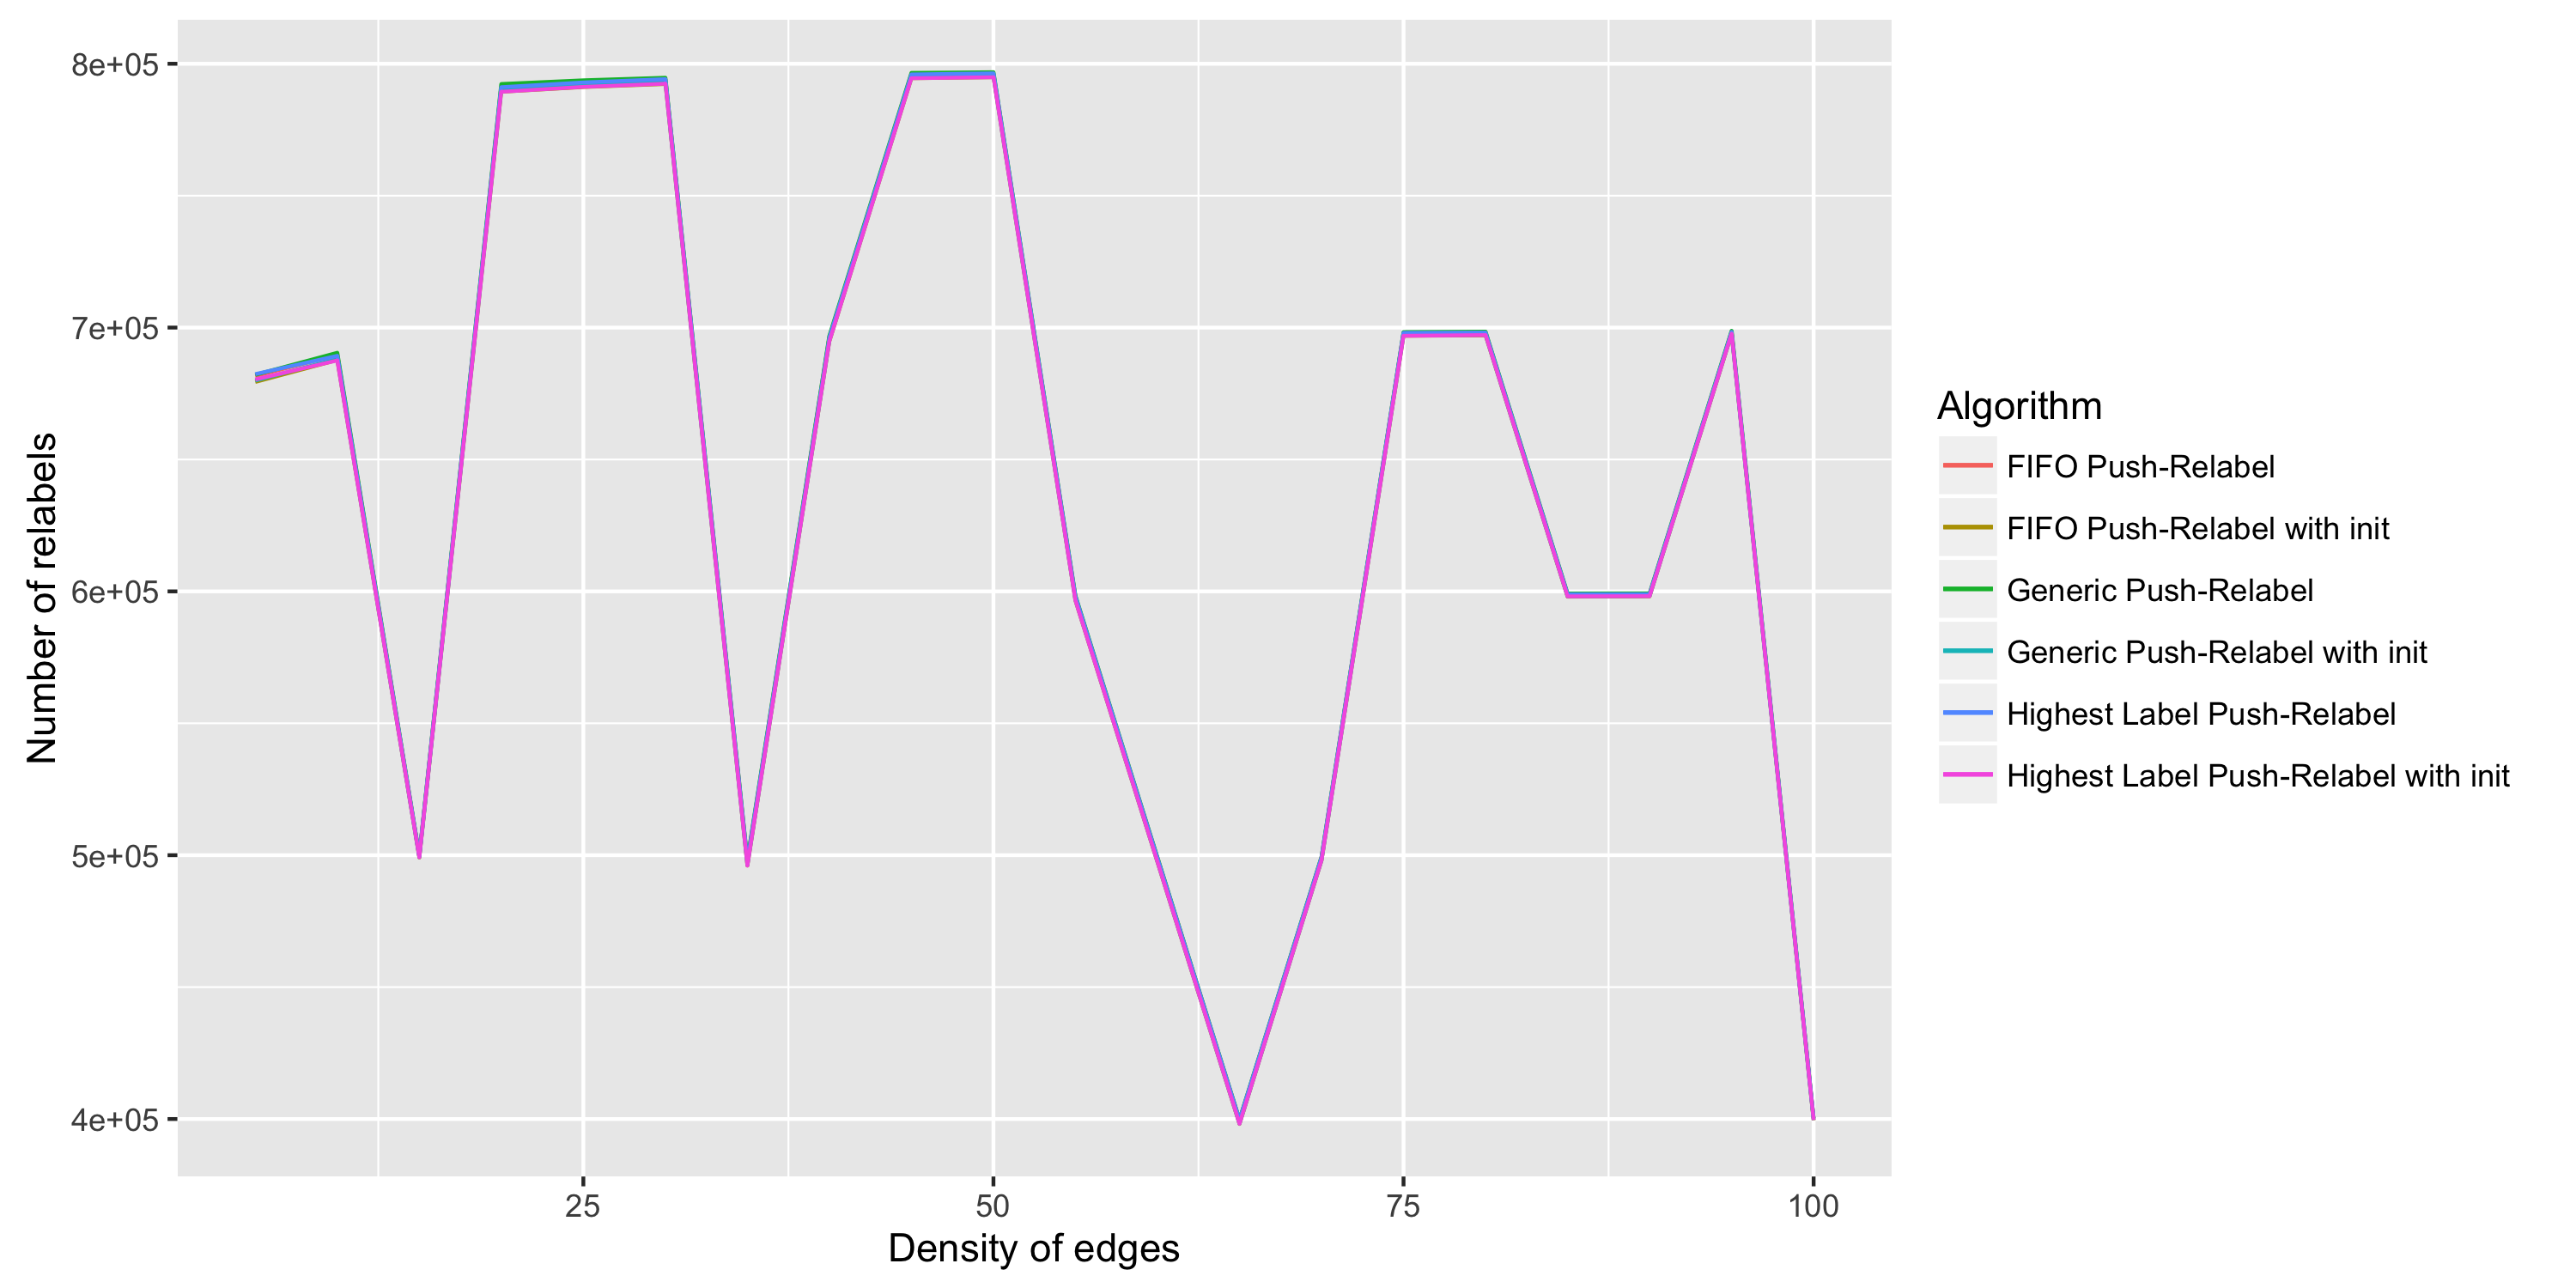
\includegraphics[scale=0.13]{images/meanrelabels.png}
\caption{The mean number of relabels in density variation instances.}
\label{fig:mean_relabel}
\end{center}
\end{figure}

As we can see in the Figure~\ref{fig:mean_relabel} we can observe what we said in the Section~\ref{sec:hauteurs} in term of relabels. The number of relabels is not affected by the fact we initialize or not the height label in the preflow phase of the algorithm. The reason of this is explained in the Section~\ref{sec:hauteurs}.

\subsubsection{Saturing push}
\begin{figure}[H]
\begin{center}
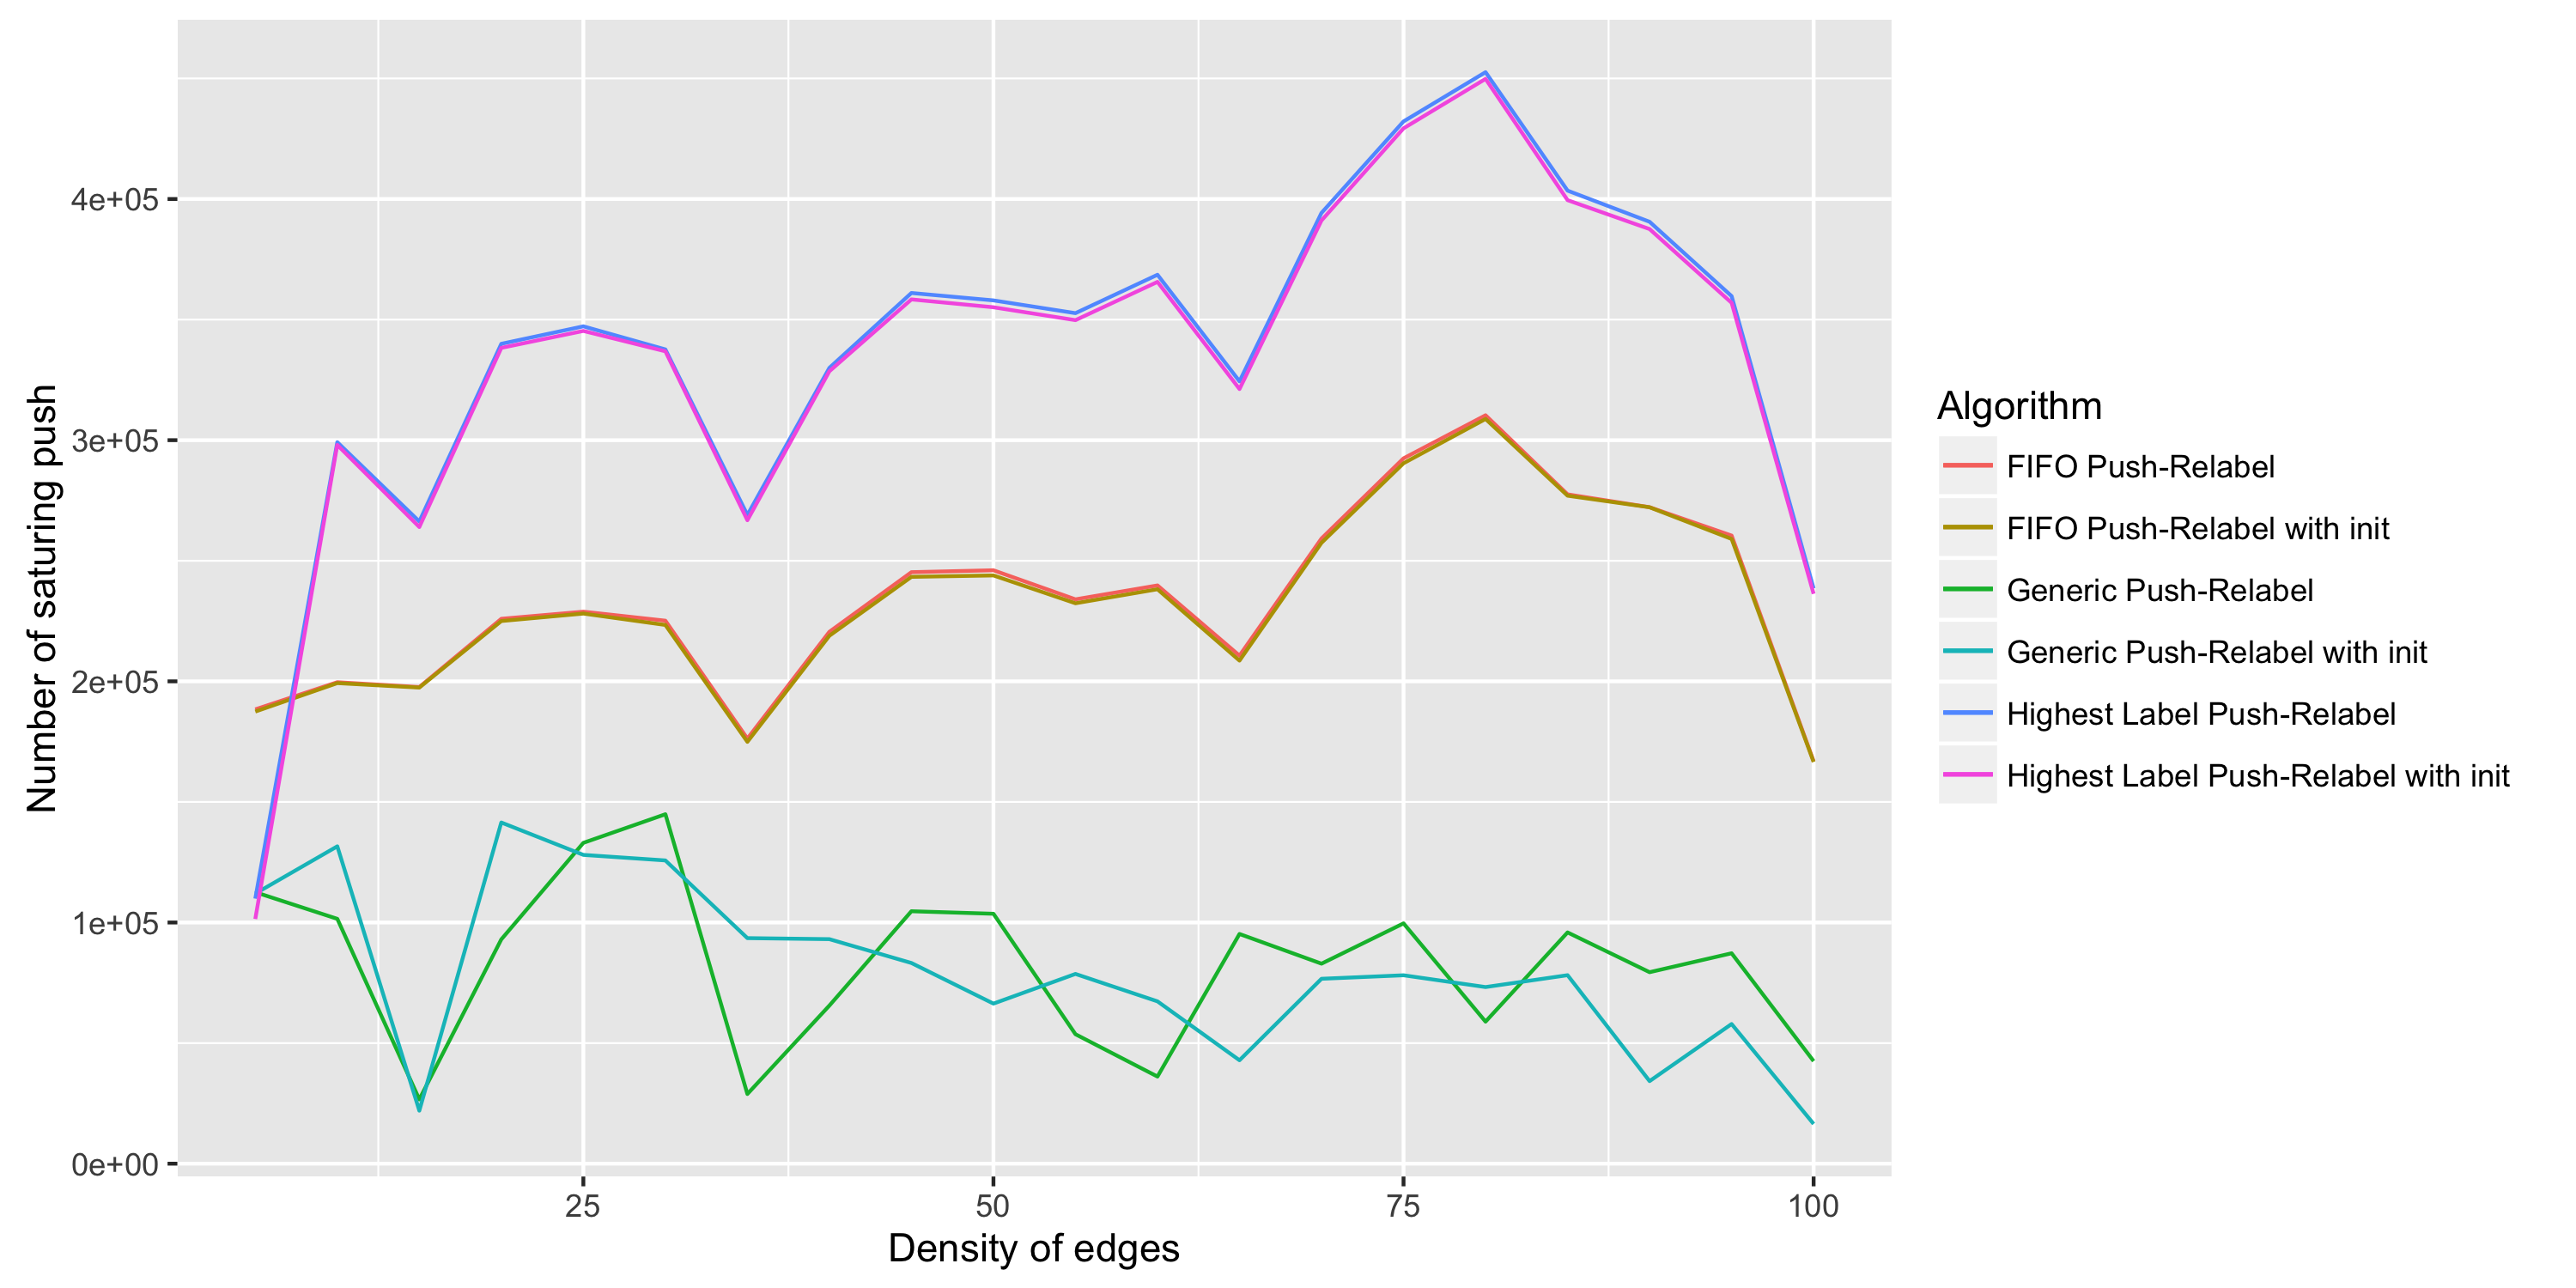
\includegraphics[scale=0.13]{images/meansaturingpushes.png}
\caption{The mean number of saturing pushes in density variation instances.}
\label{fig:mean_sat}
\end{center}
\end{figure}

We can observe in Figure~\ref{fig:mean_sat} that for each heuristic, the initialization is slightly beneficial in term of the number of saturing pushes. The highest label heuristic perfoms more saturing push than the FIFO heuritic, and the generic algorithm performs less saturing push than the two others.


\subsubsection{Non-saturing push}

\begin{figure}[H]
\begin{center}
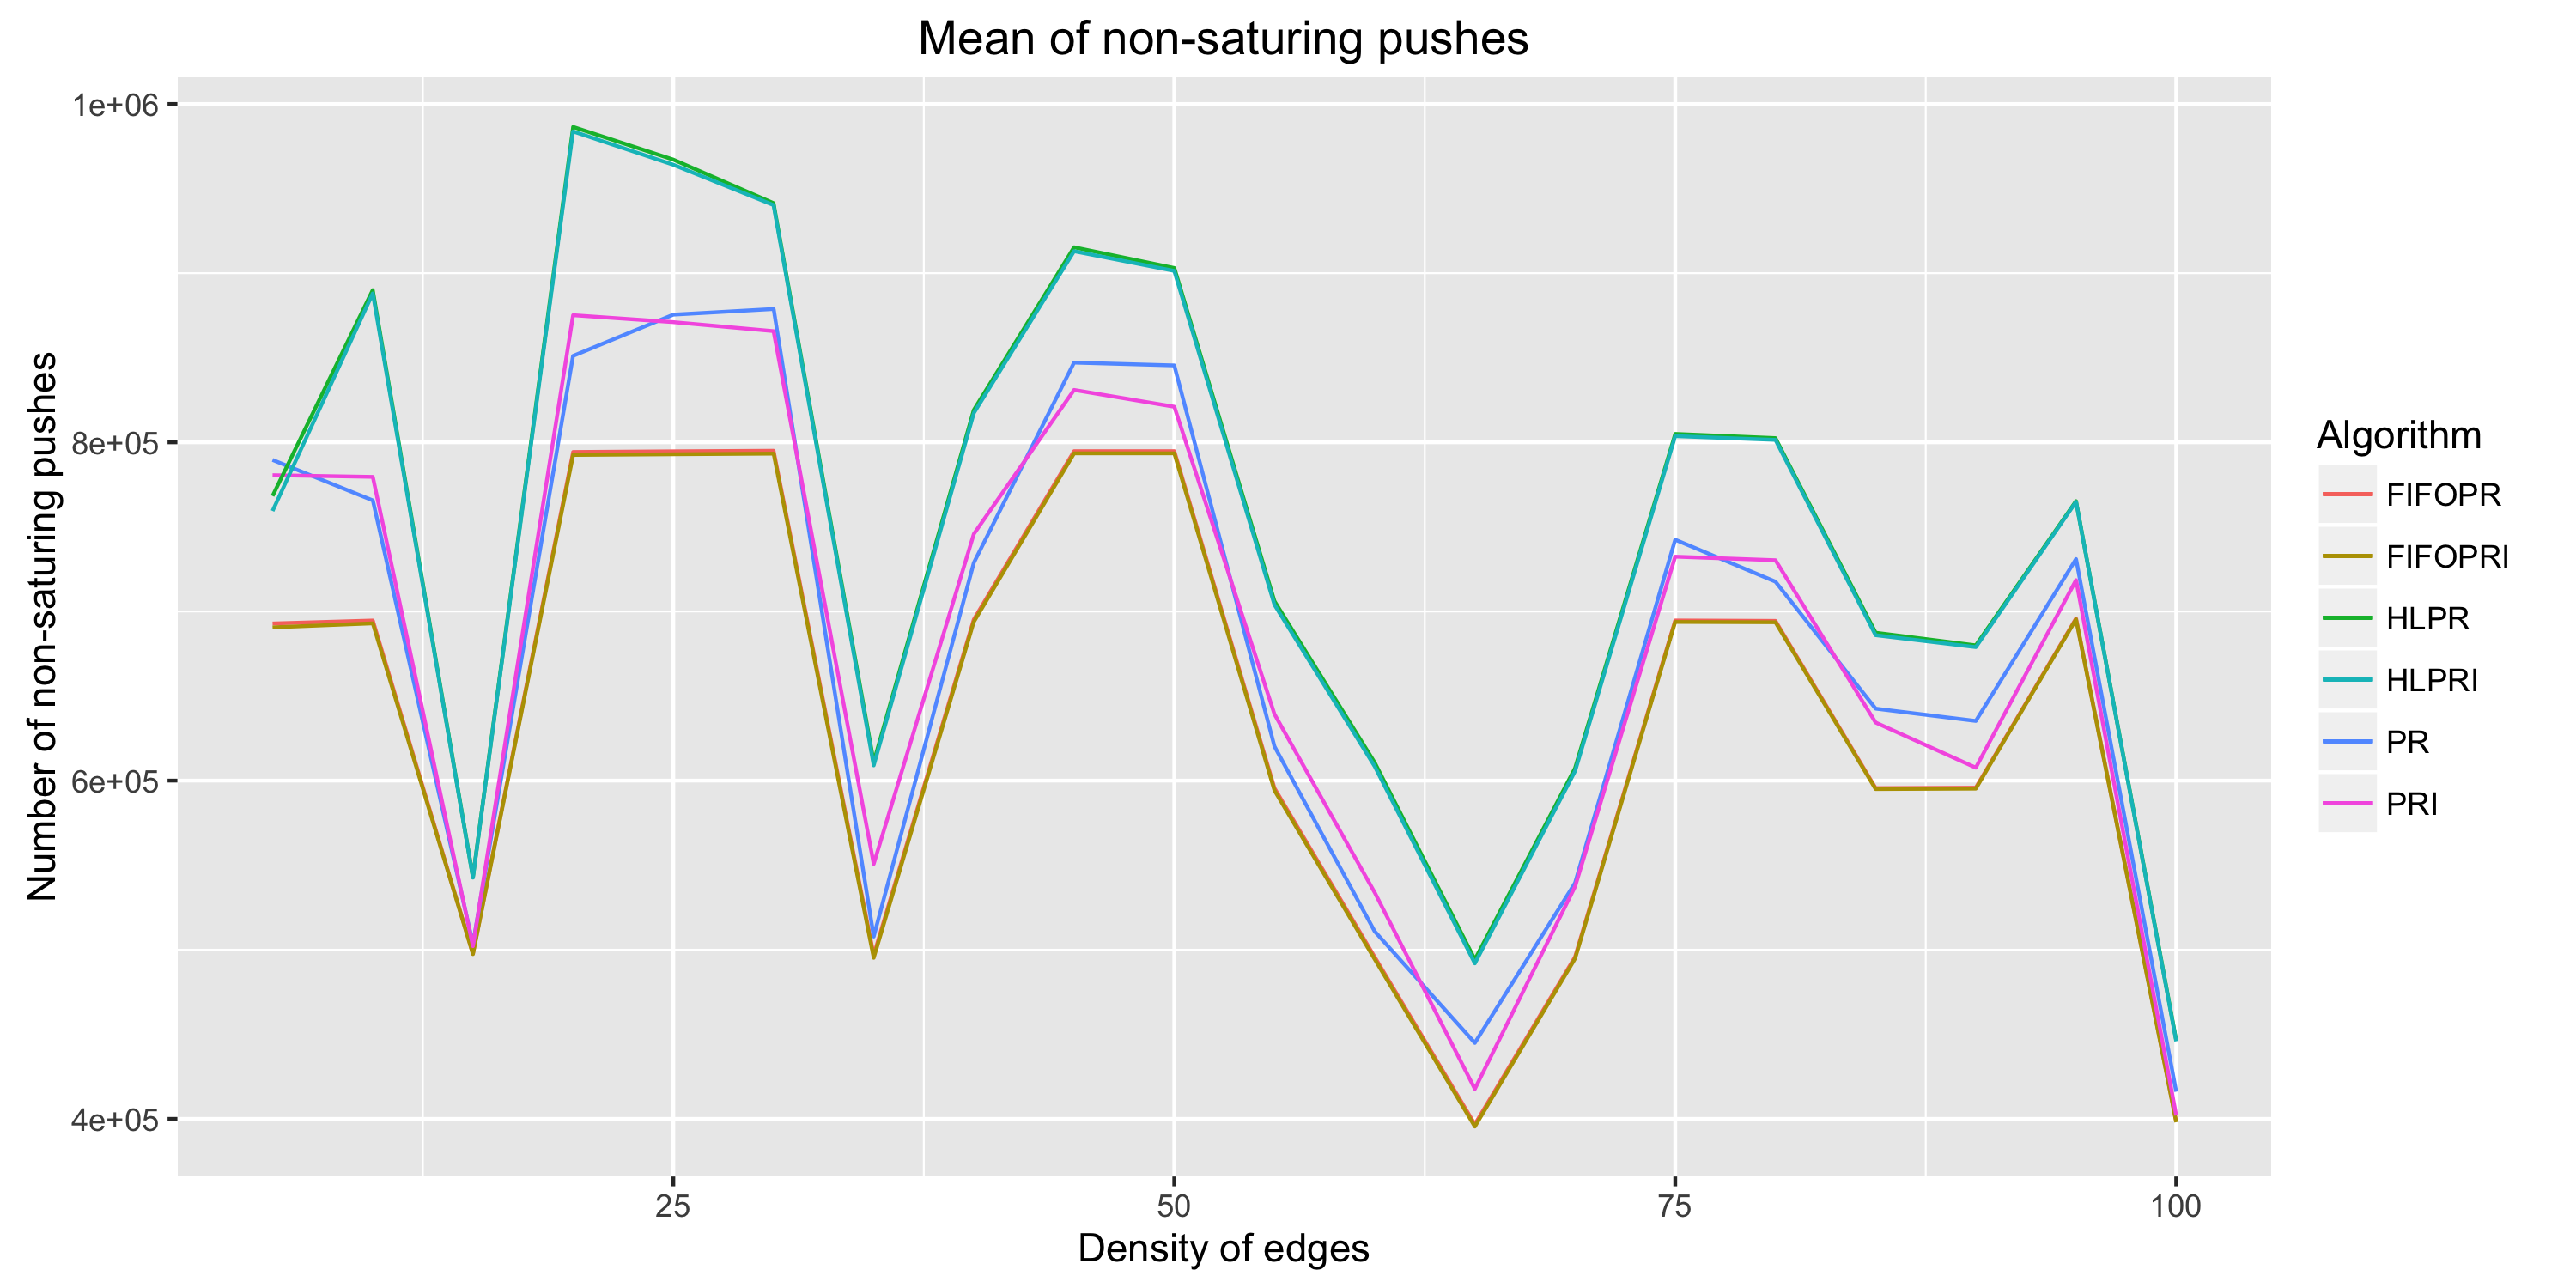
\includegraphics[scale=0.13]{images/meannonsaturingpushes.png}
\caption{The mean number of non-saturing pushes in density variation instances.}
\label{fig:mean_non_sat}
\end{center}
\end{figure}

As for the saturing push, the number of non-saturing push slightly decrease when we do an initialization of the height labels. The highest label heuristic decreases the number of non-saturing push in regards to the generic algorithm. The FIFO heuristic tend to augment this number of push.


\subsection{Best Push-Relabel}

In this section, we will compare the run time of each algorithm on different kinds of instances.

\subsubsection{Density variation instances}
\begin{figure}[H]
\begin{center}
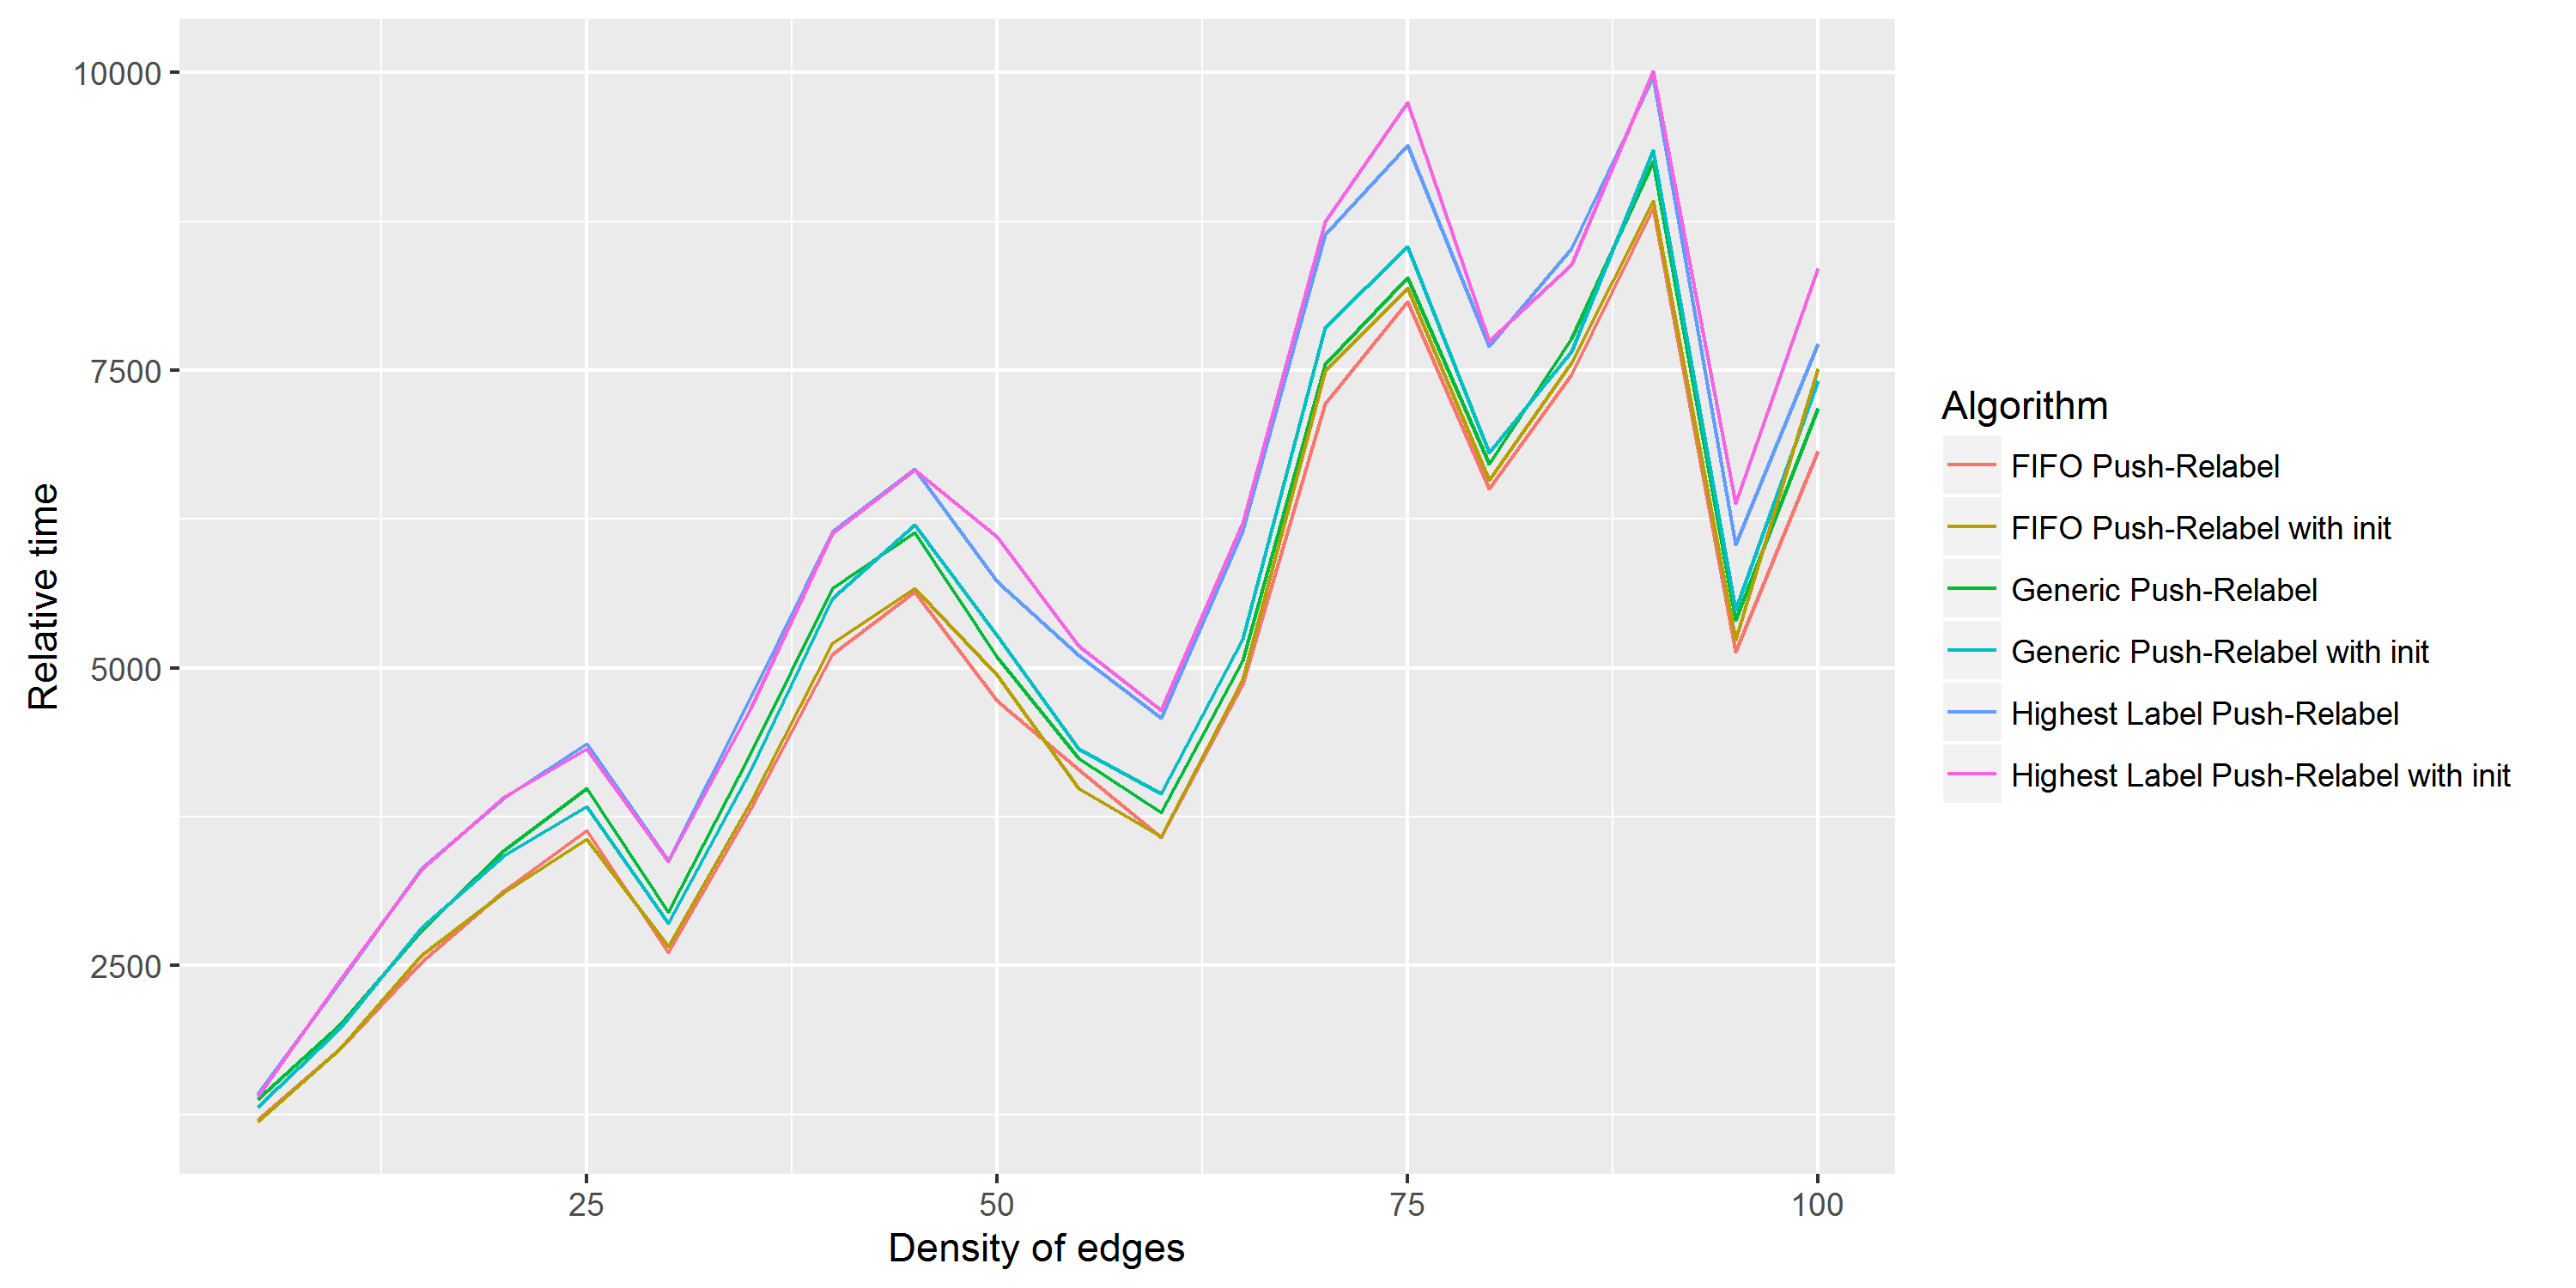
\includegraphics[scale=0.5]{images/meandensitypr.png}
\caption{The execution time of the different push relabels by density.}
\label{fig:mean_density_pr}
\end{center}
\end{figure}

We can see here that the \textit{FIFOPushRelabel} is the fastest. For each heuristic, it is interesting to see that the initialization phase does not make the resolution of the problem faster. 
\subsubsection{Size variation instances}
\begin{figure}[H]
\begin{center}
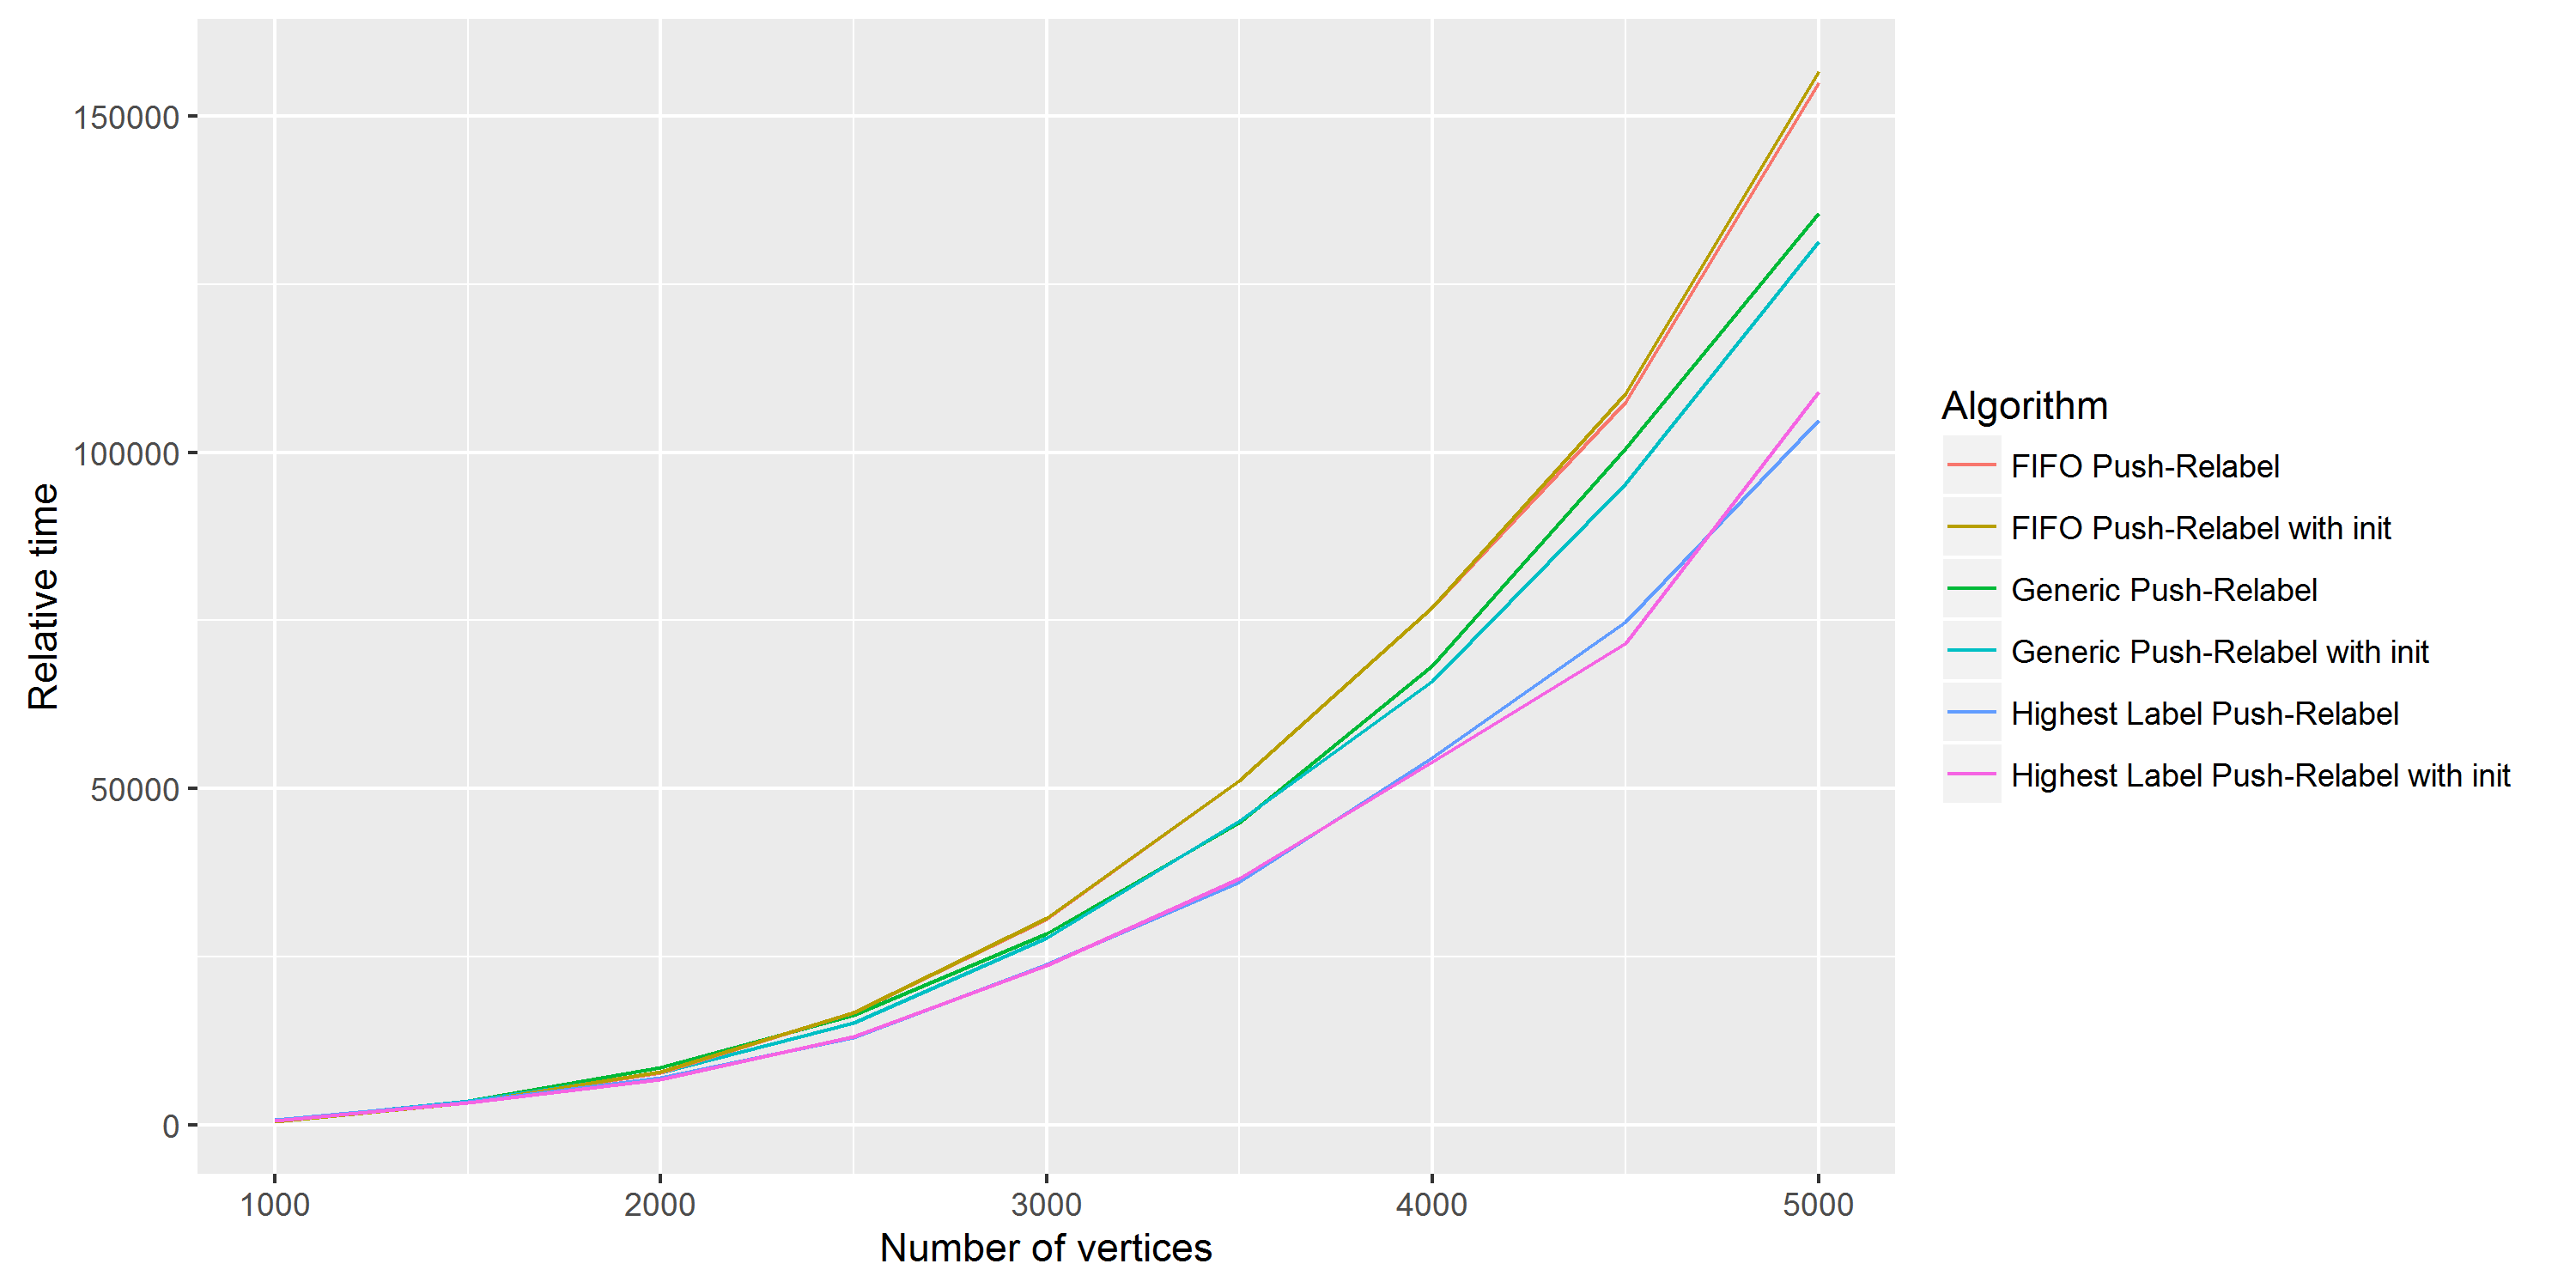
\includegraphics[scale=0.5]{images/meansizepr.png}
\caption{The execution time of the different push relabels by size.}
\label{fig:mean_size_pr}
\end{center}
\end{figure}

When changing the size of the network, we can see that the highest label heuristic perform the best. The initialization of the algorithm does not seem to change a lot the computation time of each heuritic. In this case, it's the highest label heuristic faster.
%TODO Analyse?


\subsubsection{Matching problem instances}
\begin{figure}[H]
\begin{center}
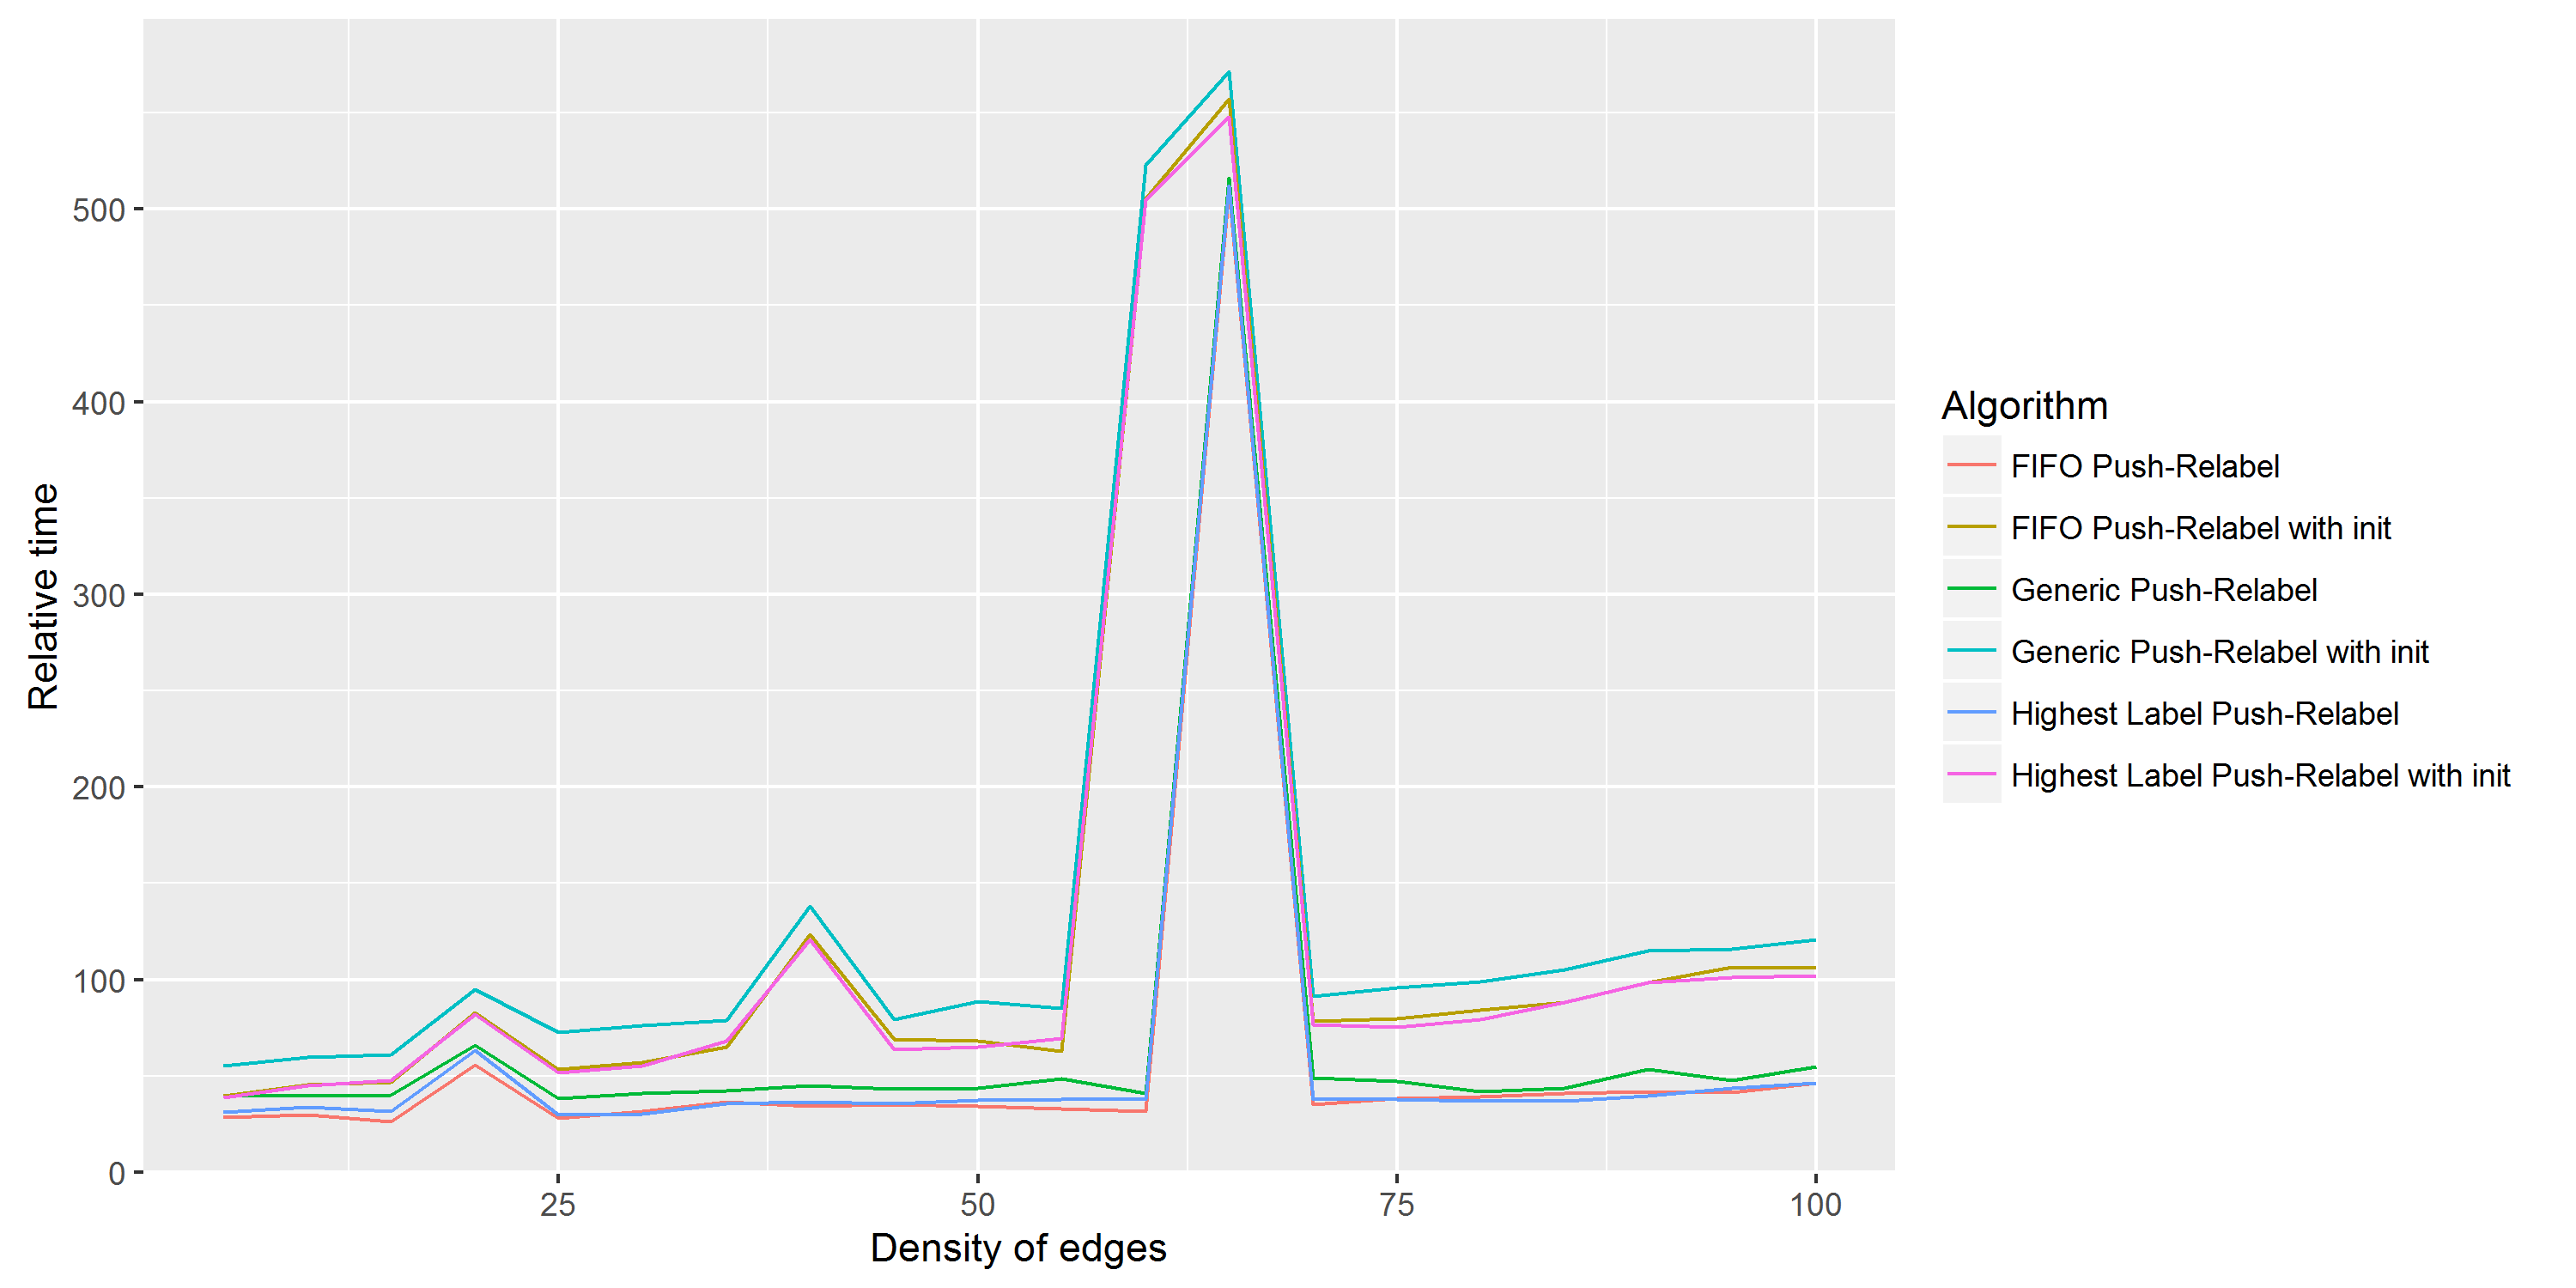
\includegraphics[scale=0.5]{images/meanmatchingpr.png}
\caption{The execution time of the different push relabels on the matching problem instances.}
\label{fig:mean_matching_pr}
\end{center}
\end{figure}

Here, we can observe that the initialization phase make each heuristic slower. It is because the problem here is simpler and very quick to resolve, thus, the initialization phase take a more important place in the result. The spike on the graph is caused by the data structure used, the \textit{sparsemap}. Here, the high label heuristic is the best as well.


\section{Data structures}
In this section, we would like to determine which data structure is the most adapted for our algorithms.
\subsection{Push-Relabel}	
The Figure \ref{fig:prmeandensity}, \ref{fig:prmeansize} and \ref{fig:prmeanmatching} represents the average run time of all data structures with Highest Label Push-Relabel. They were computed on, respectively, the density variation, the size variation and the matching problem instances.
\begin{figure}[H]
\begin{center}
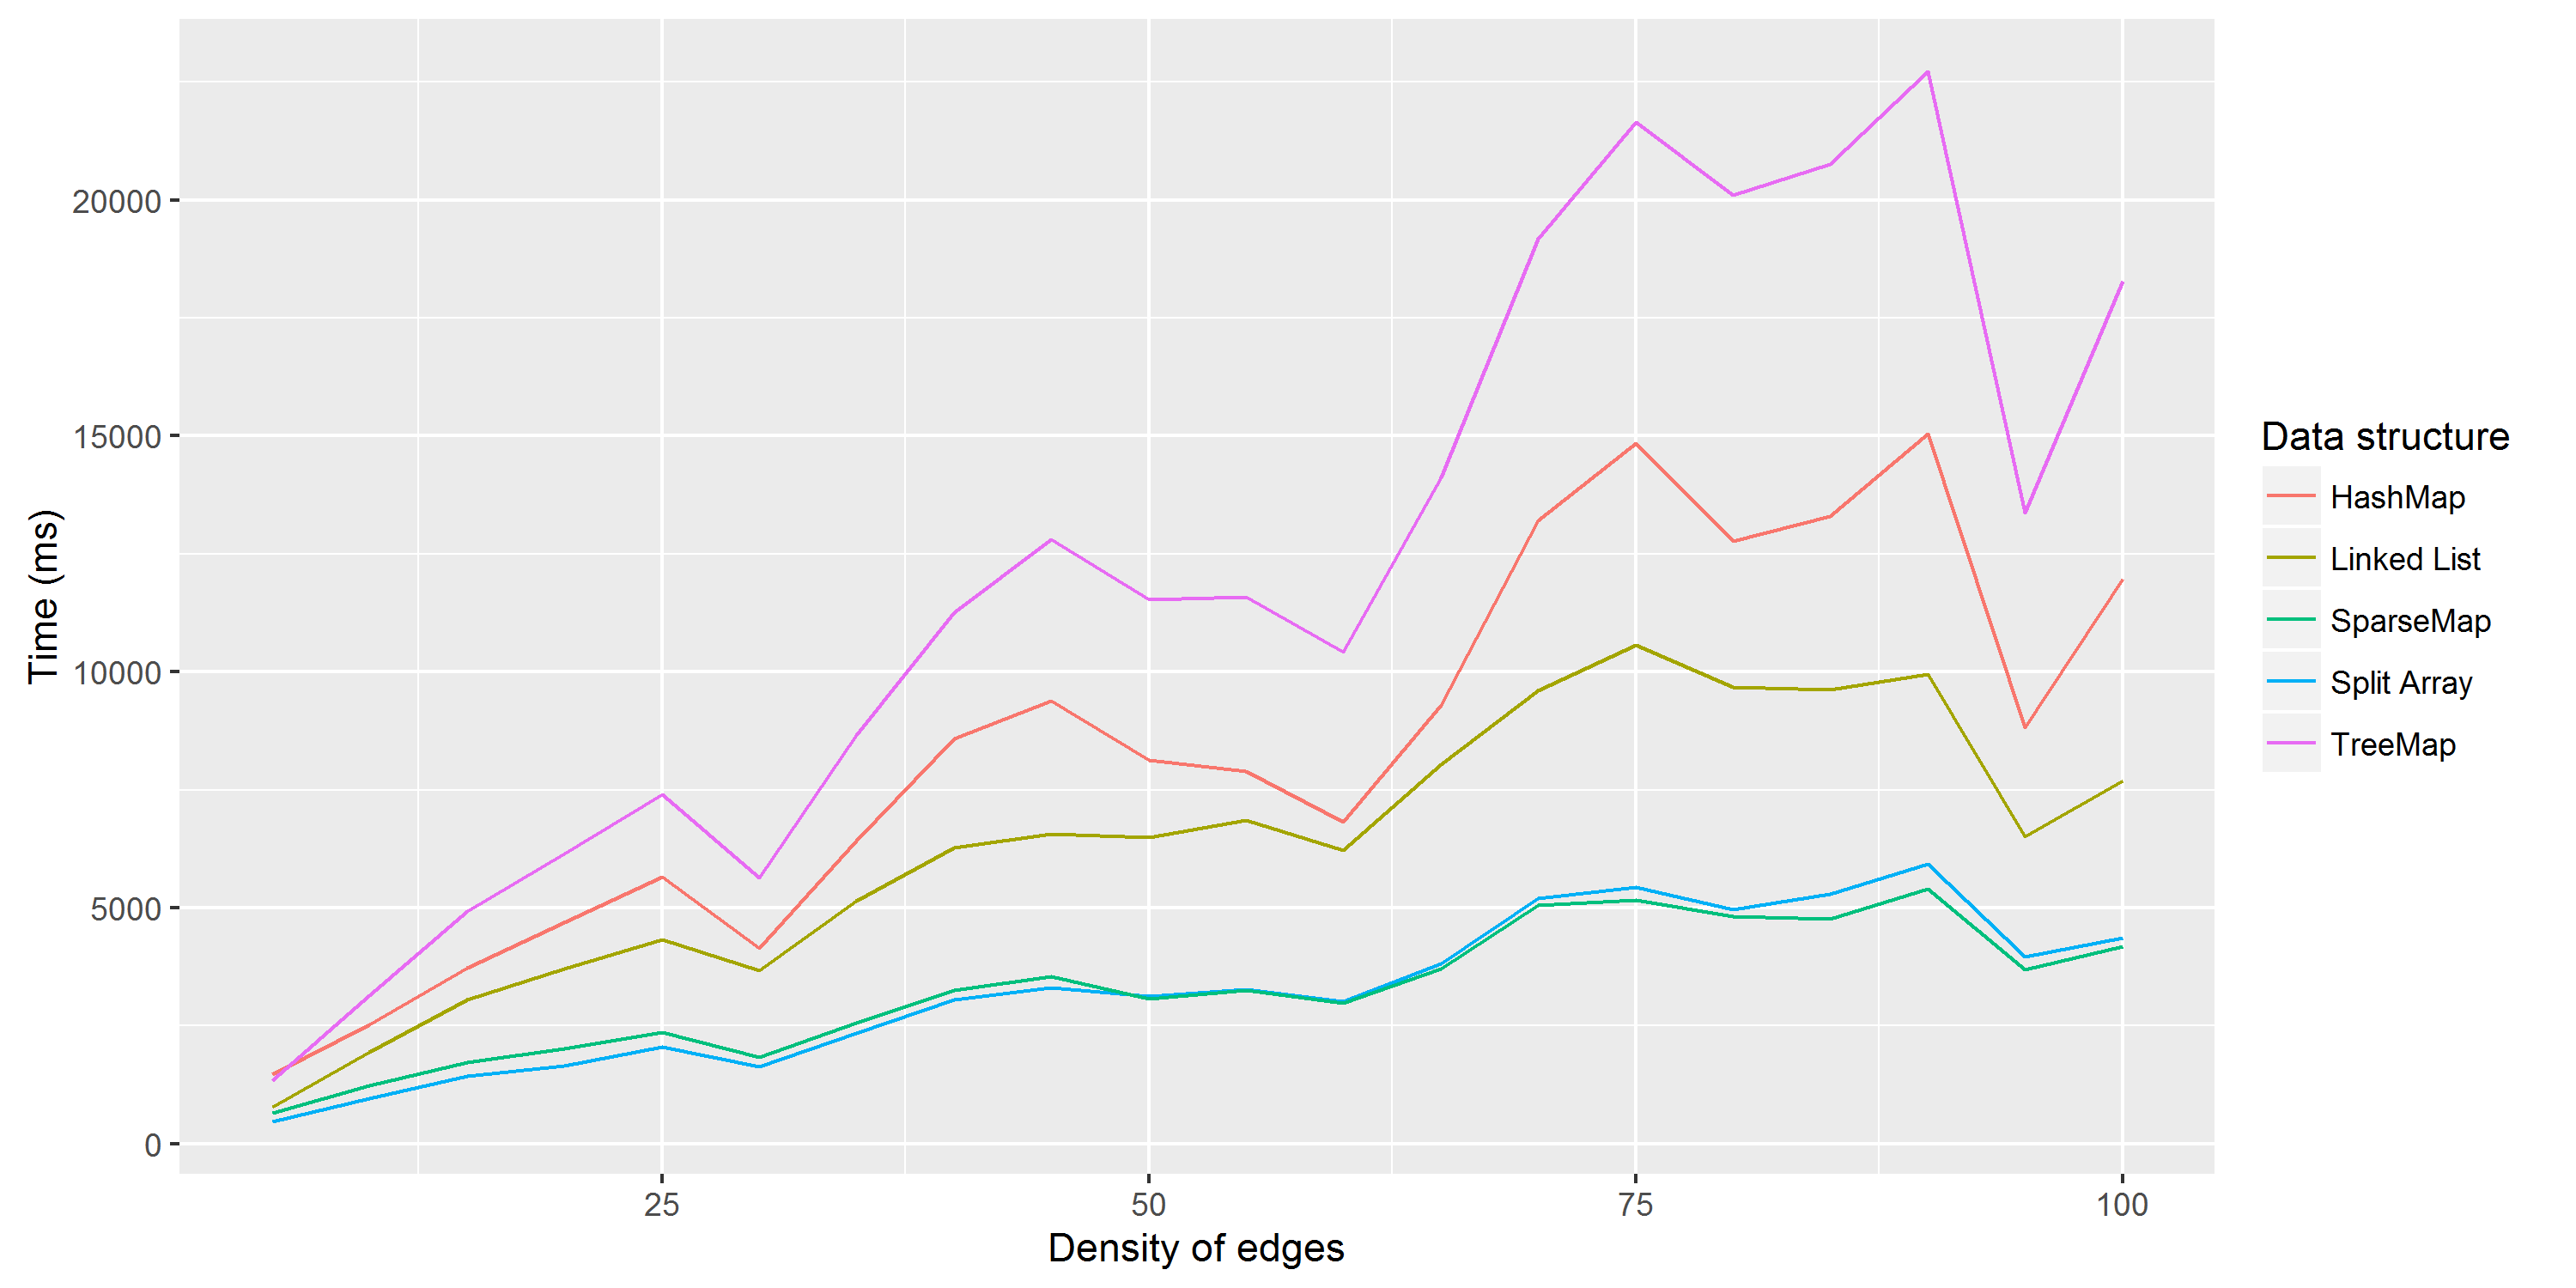
\includegraphics[scale=0.5]{images/results/prmeandensity.png}
\caption{Average run time of all data structures with Highest Label Push-Relabel on density variation instances.}
\label{fig:prmeandensity}
\end{center}
\end{figure}
\begin{figure}[H]
\begin{center}
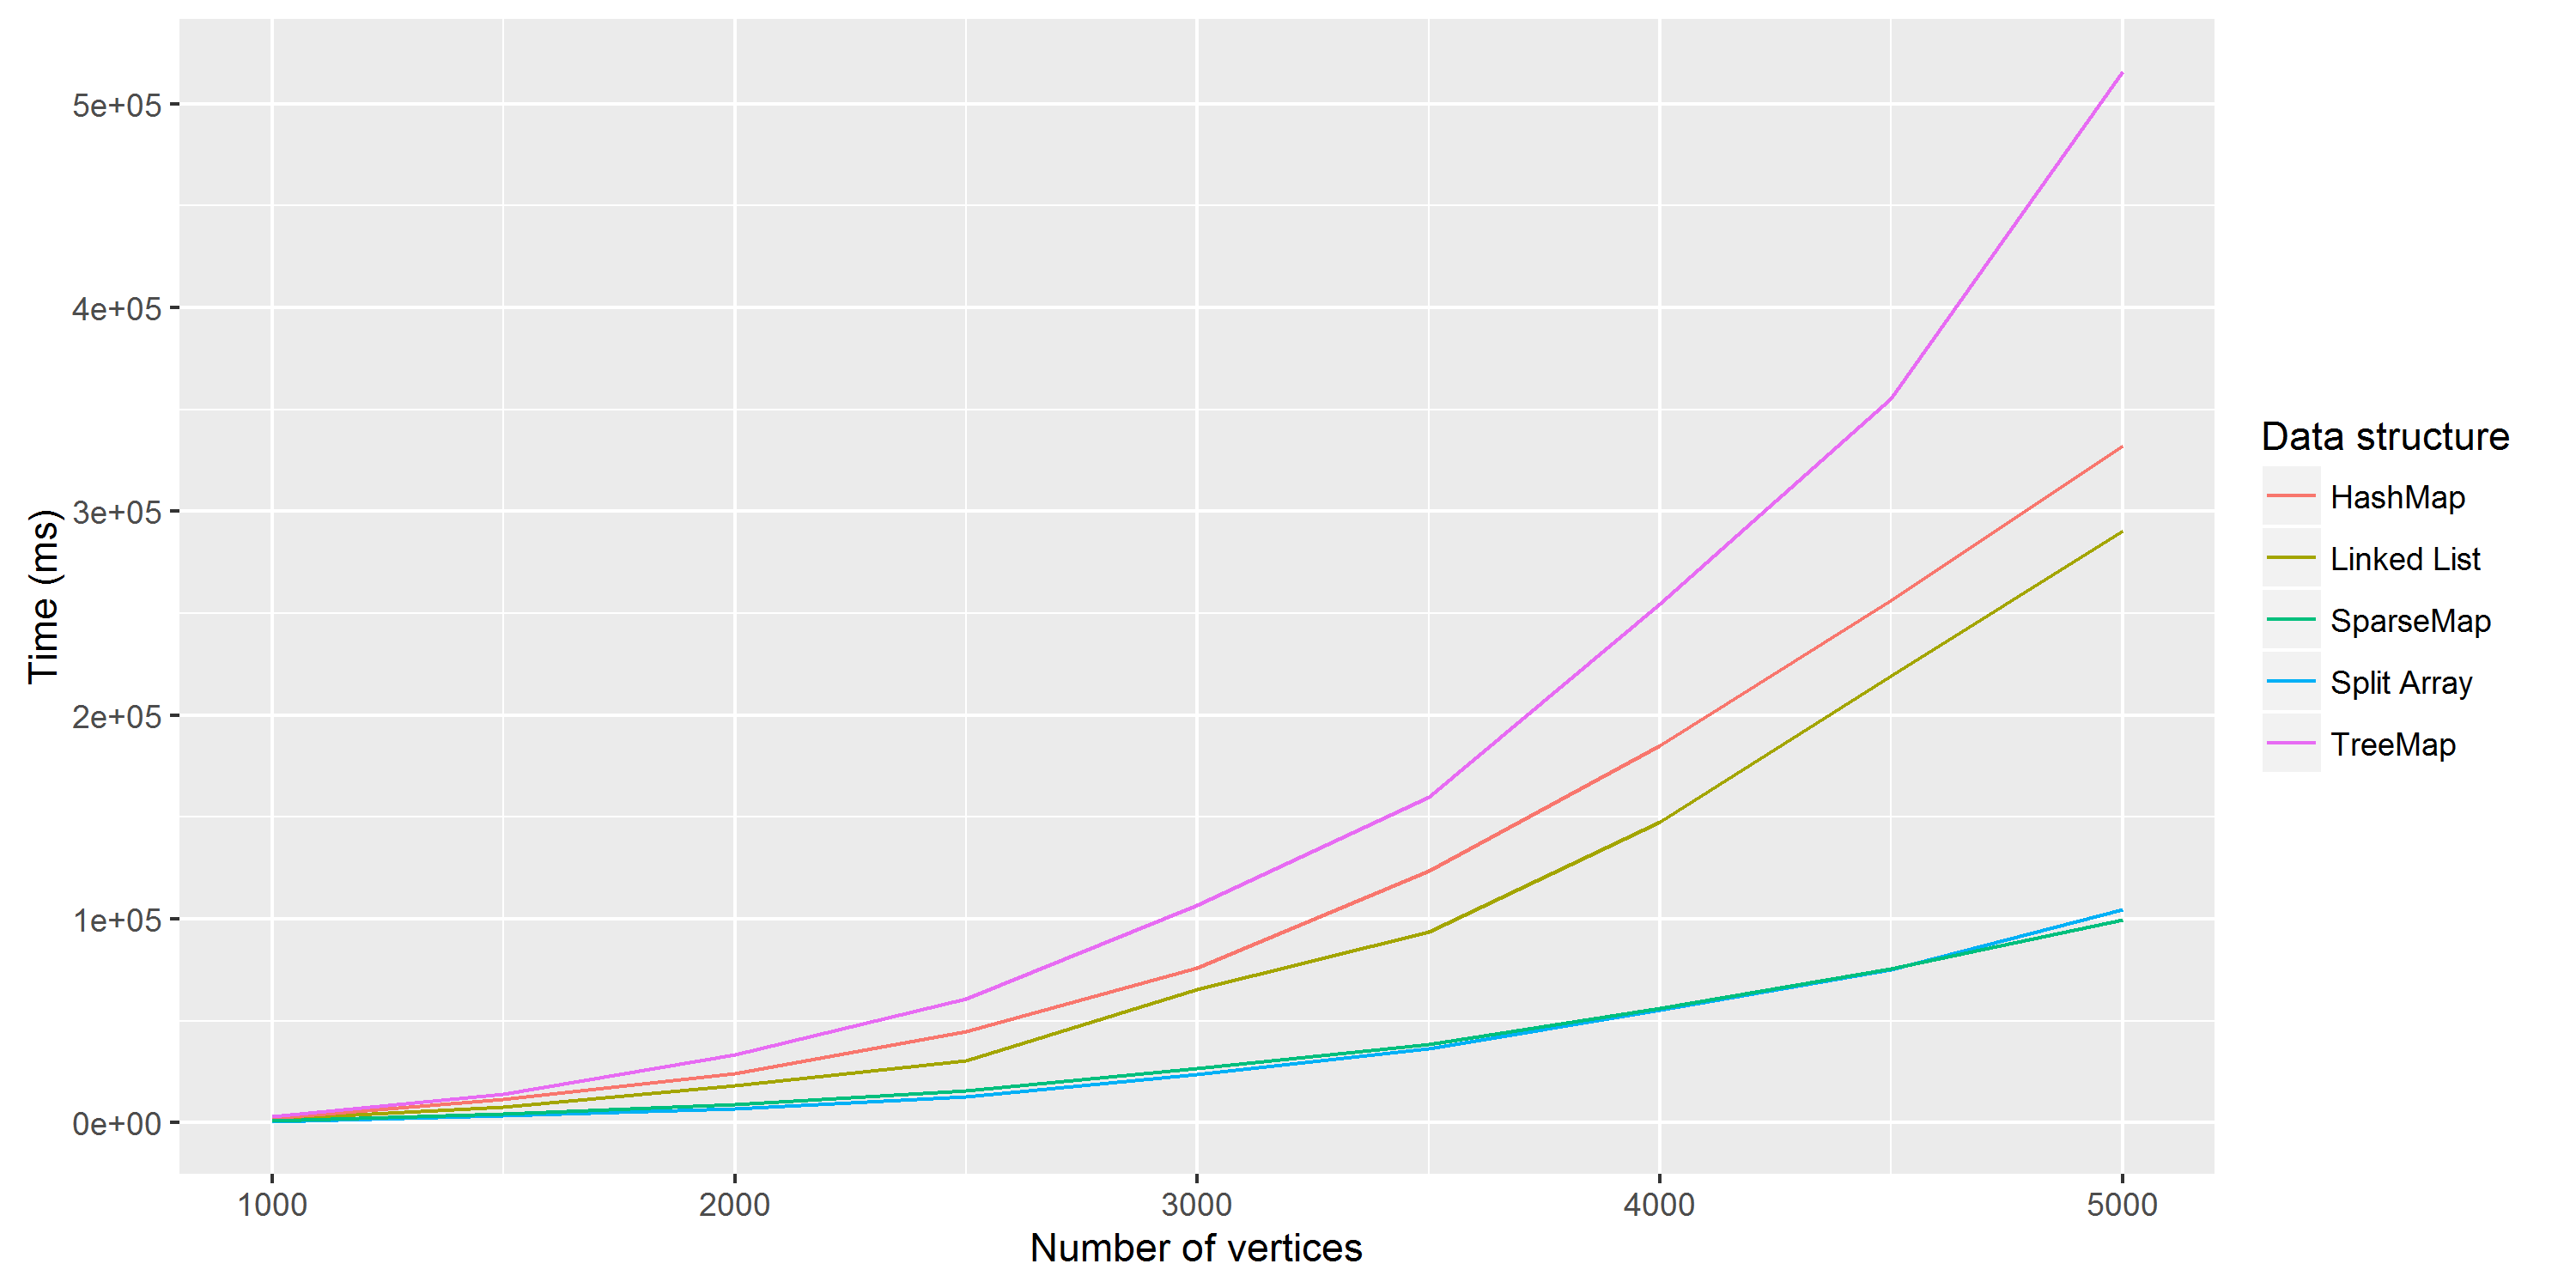
\includegraphics[scale=0.5]{images/results/prmeansize.png}
\caption{Average run time of all data structures with Highest Label Push-Relabel on size variation instances.}
\label{fig:prmeansize}
\end{center}
\end{figure}
\begin{figure}[H]
\begin{center}
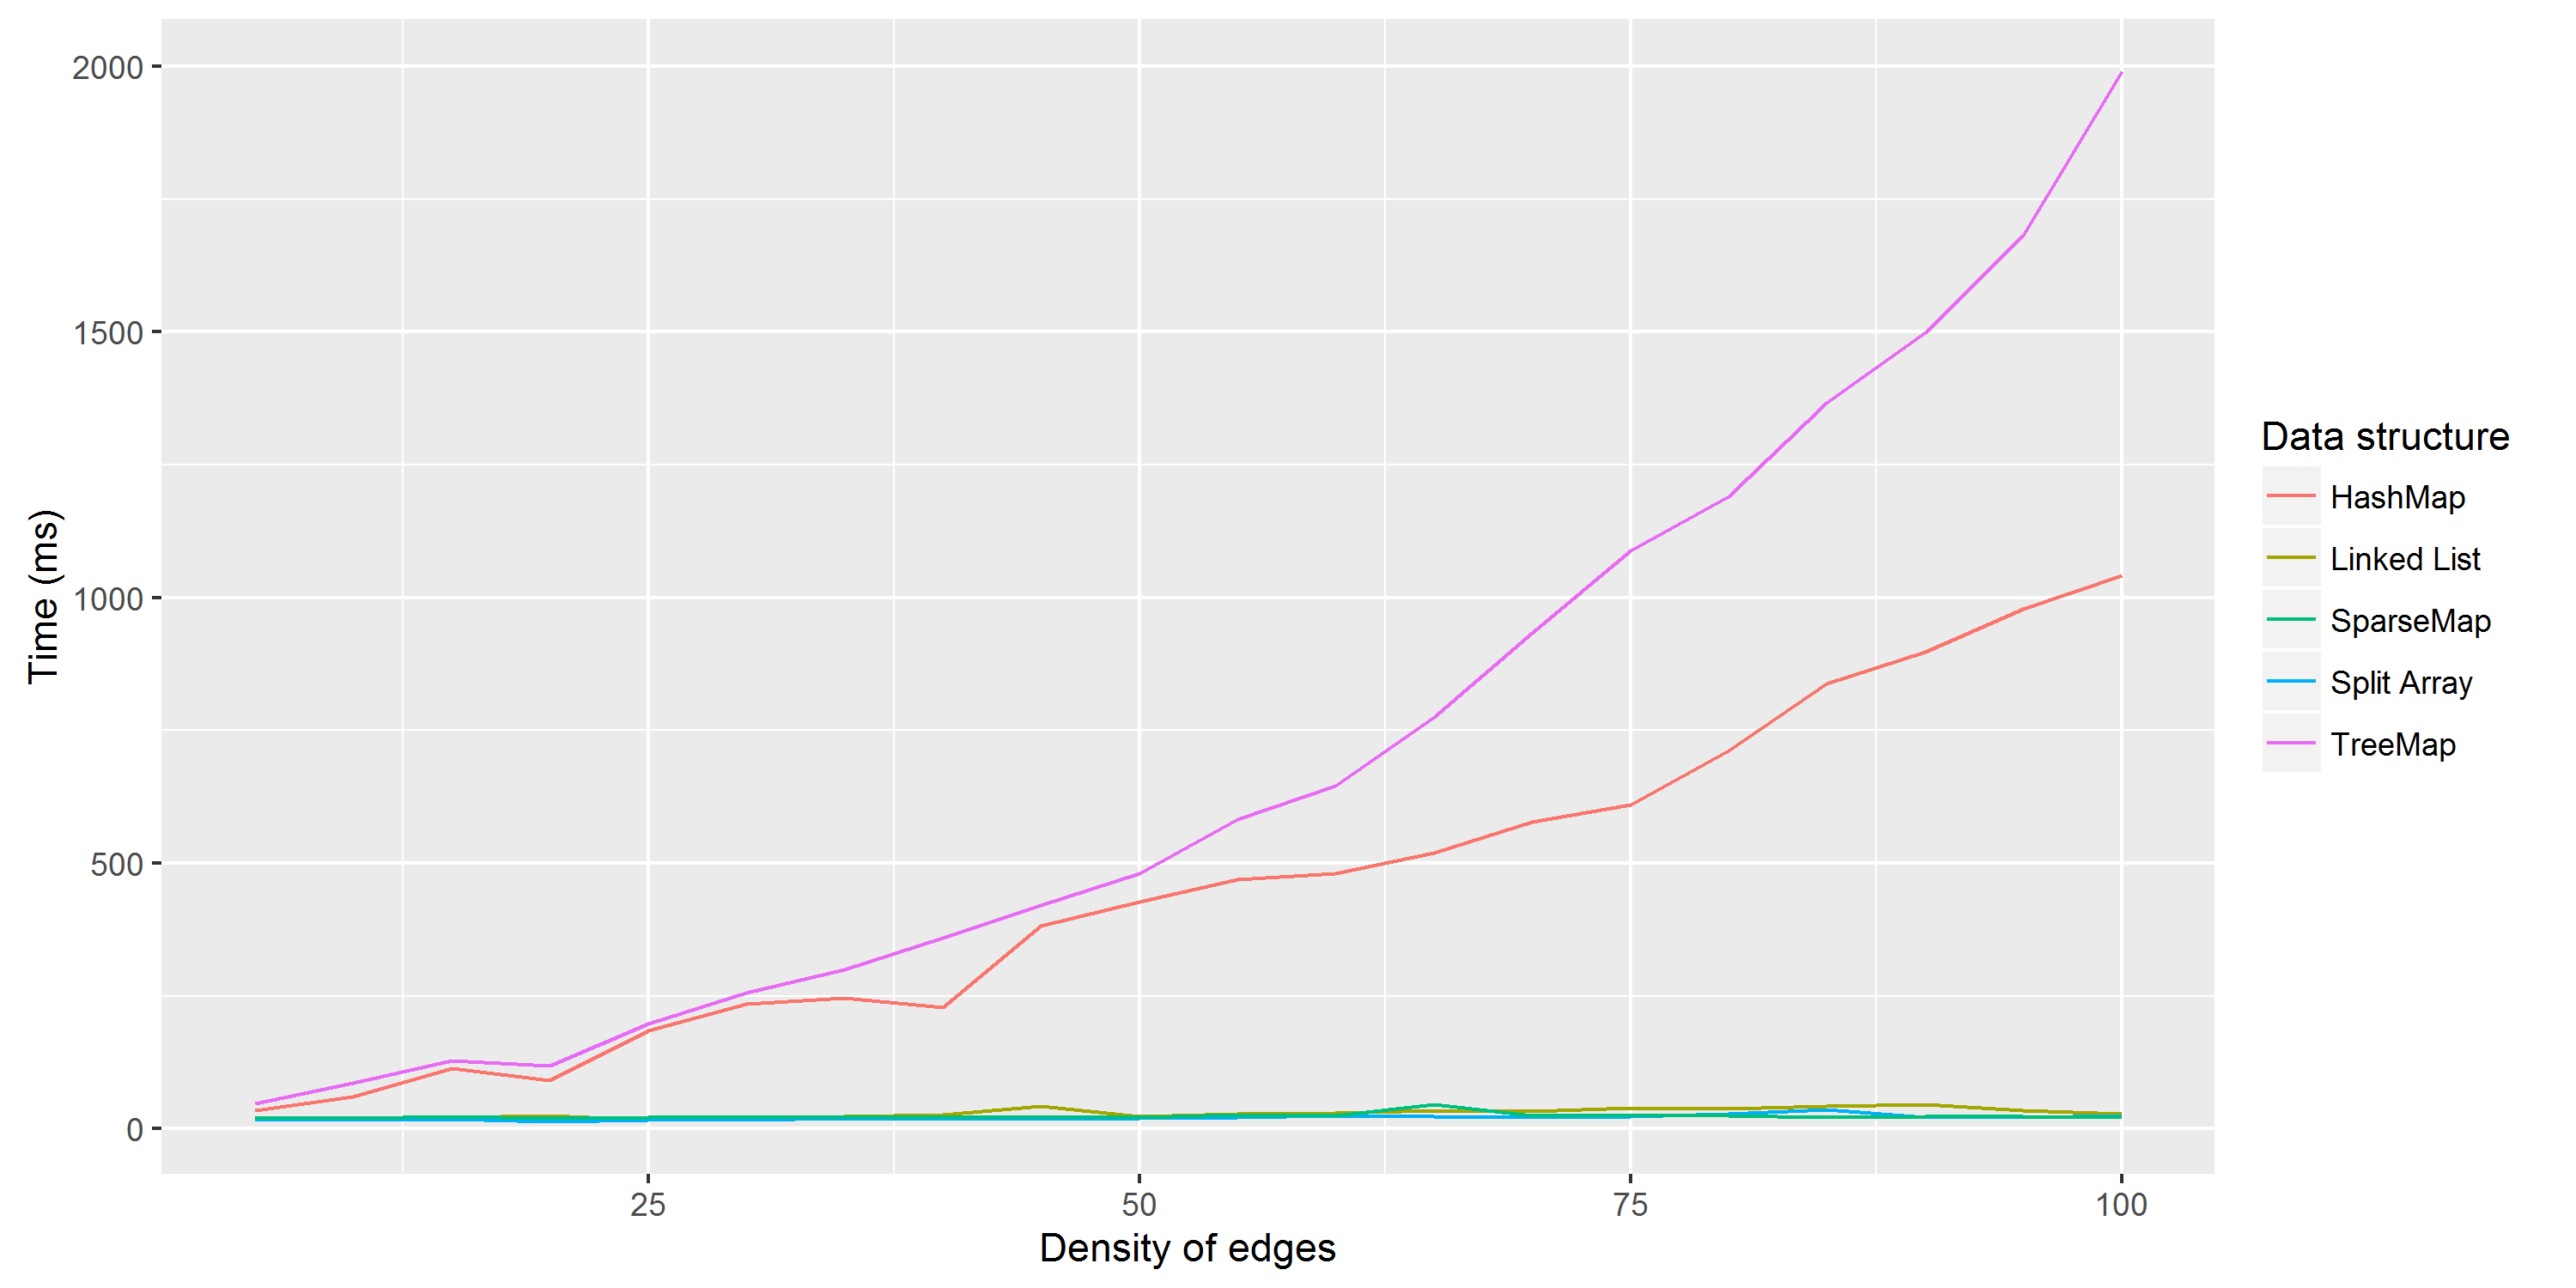
\includegraphics[scale=0.5]{images/results/prmeanmatching.png}
\caption{Average run time of all data structures with Highest Label Push-Relabel on matching instances.}
\label{fig:prmeanmatching}
\end{center}
\end{figure}

\begin{figure}[H]
\begin{center}
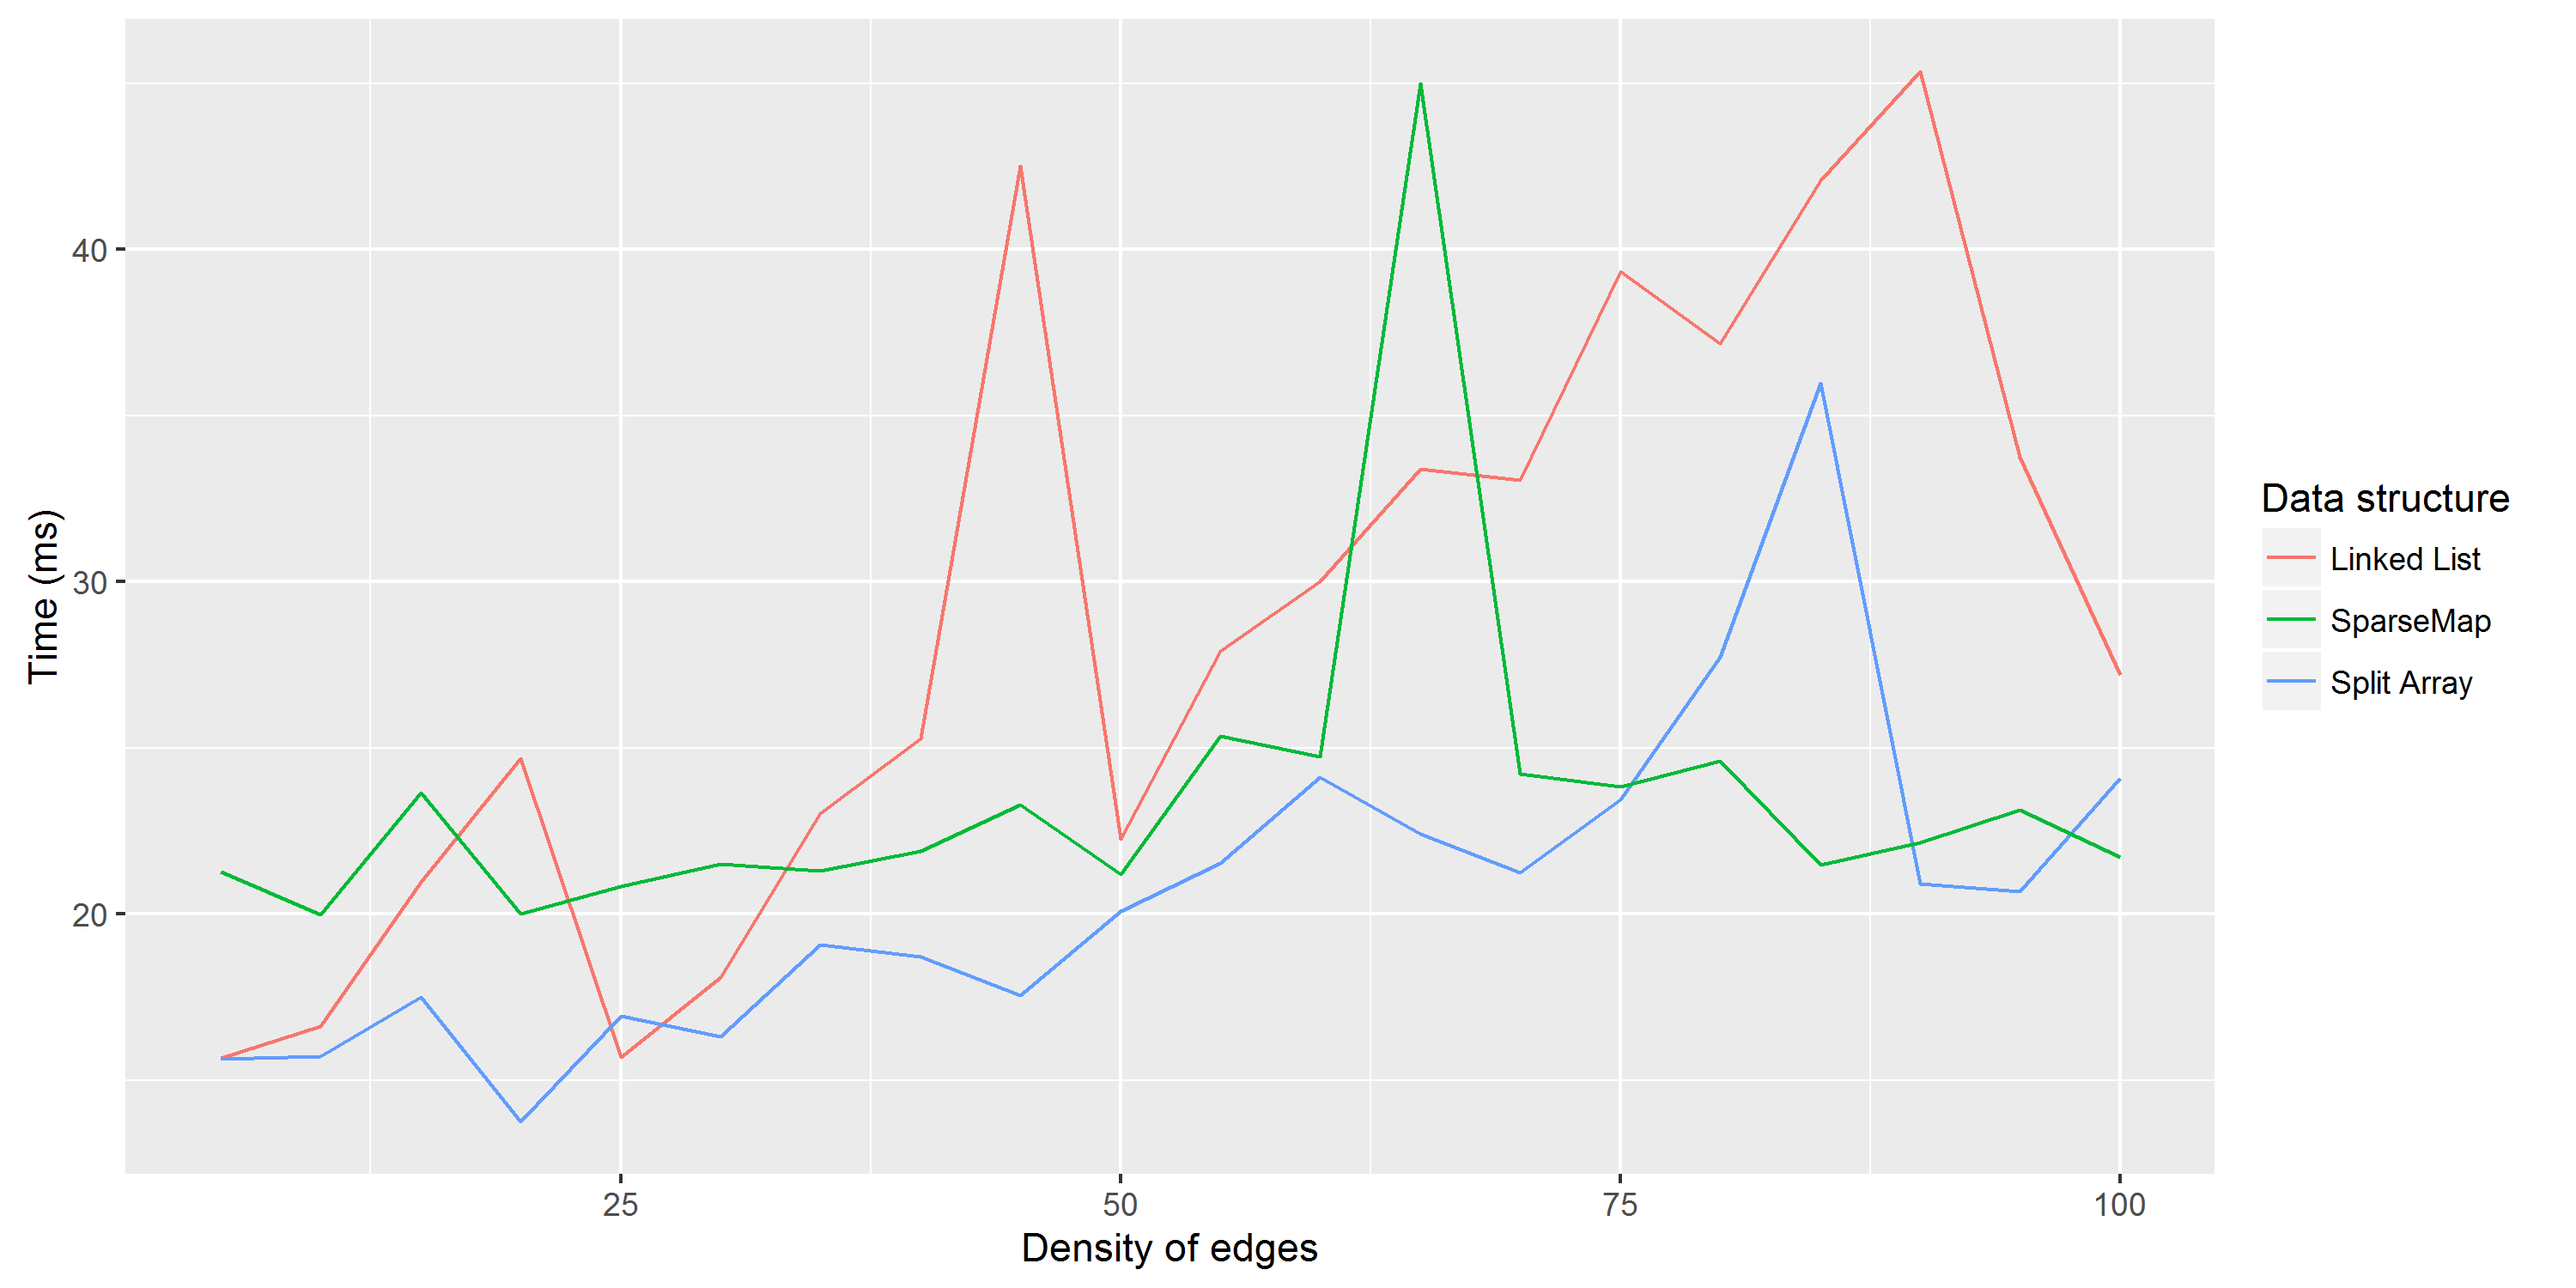
\includegraphics[scale=0.5]{images/results/prmeanmatching2.png}
\caption{Average run time of all data structures without the $hashmap$ and the$treemap$ with Highest Label Push-Relabel on matching instances.}
\label{fig:prmeanmatching}
\end{center}
\end{figure}
We notice that the $hashmap$ and the $treemap$ offer very poor performances compared to data structures based on the $sparseset$. The most adapted data structure being the $split array$.
\subsection{Edmonds-Karp}
The Figure \ref{fig:ekmeandensity}, \ref{fig:ekmeansize} and \ref{fig:ekmeanmatching} represents the average run time of all data structures with Edmonds-Karp. They were computed on, respectively, the density variation, the size variation and the matching instances.
\begin{figure}[H]
\begin{center}
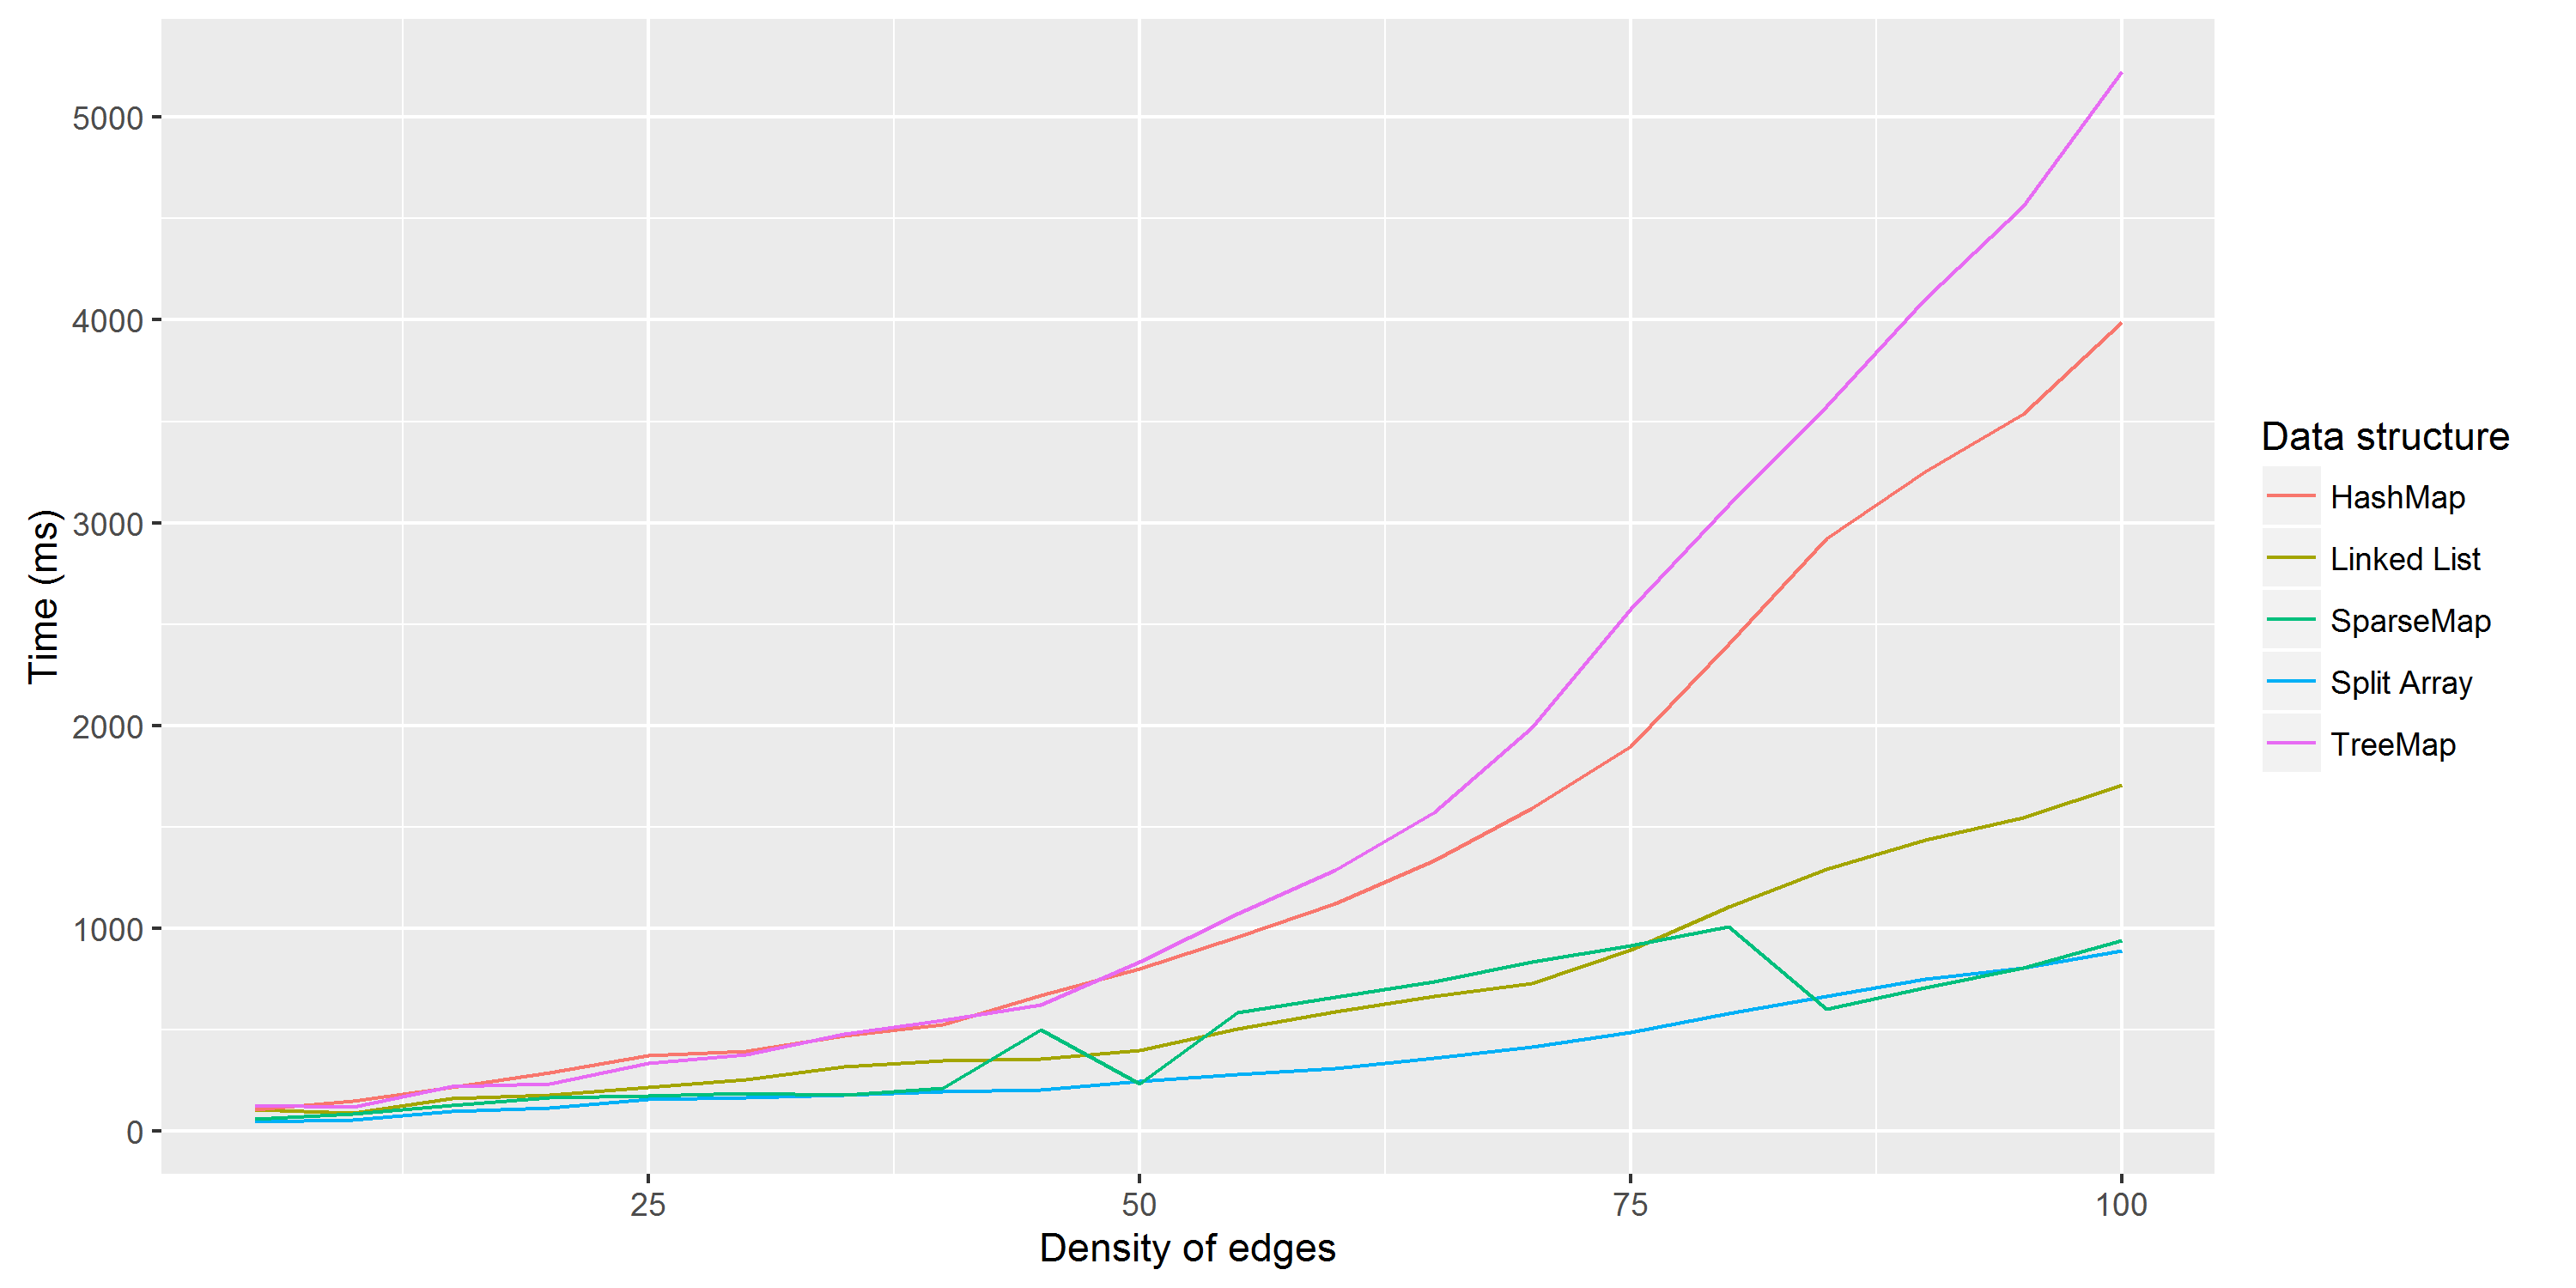
\includegraphics[scale=0.5]{images/results/ekmeandensity.png}
\caption{Average run time of all data structures with Edmonds-Karp on density variation instances.}
\label{fig:ekmeandensity}
\end{center}
\end{figure}
\begin{figure}[H]
\begin{center}
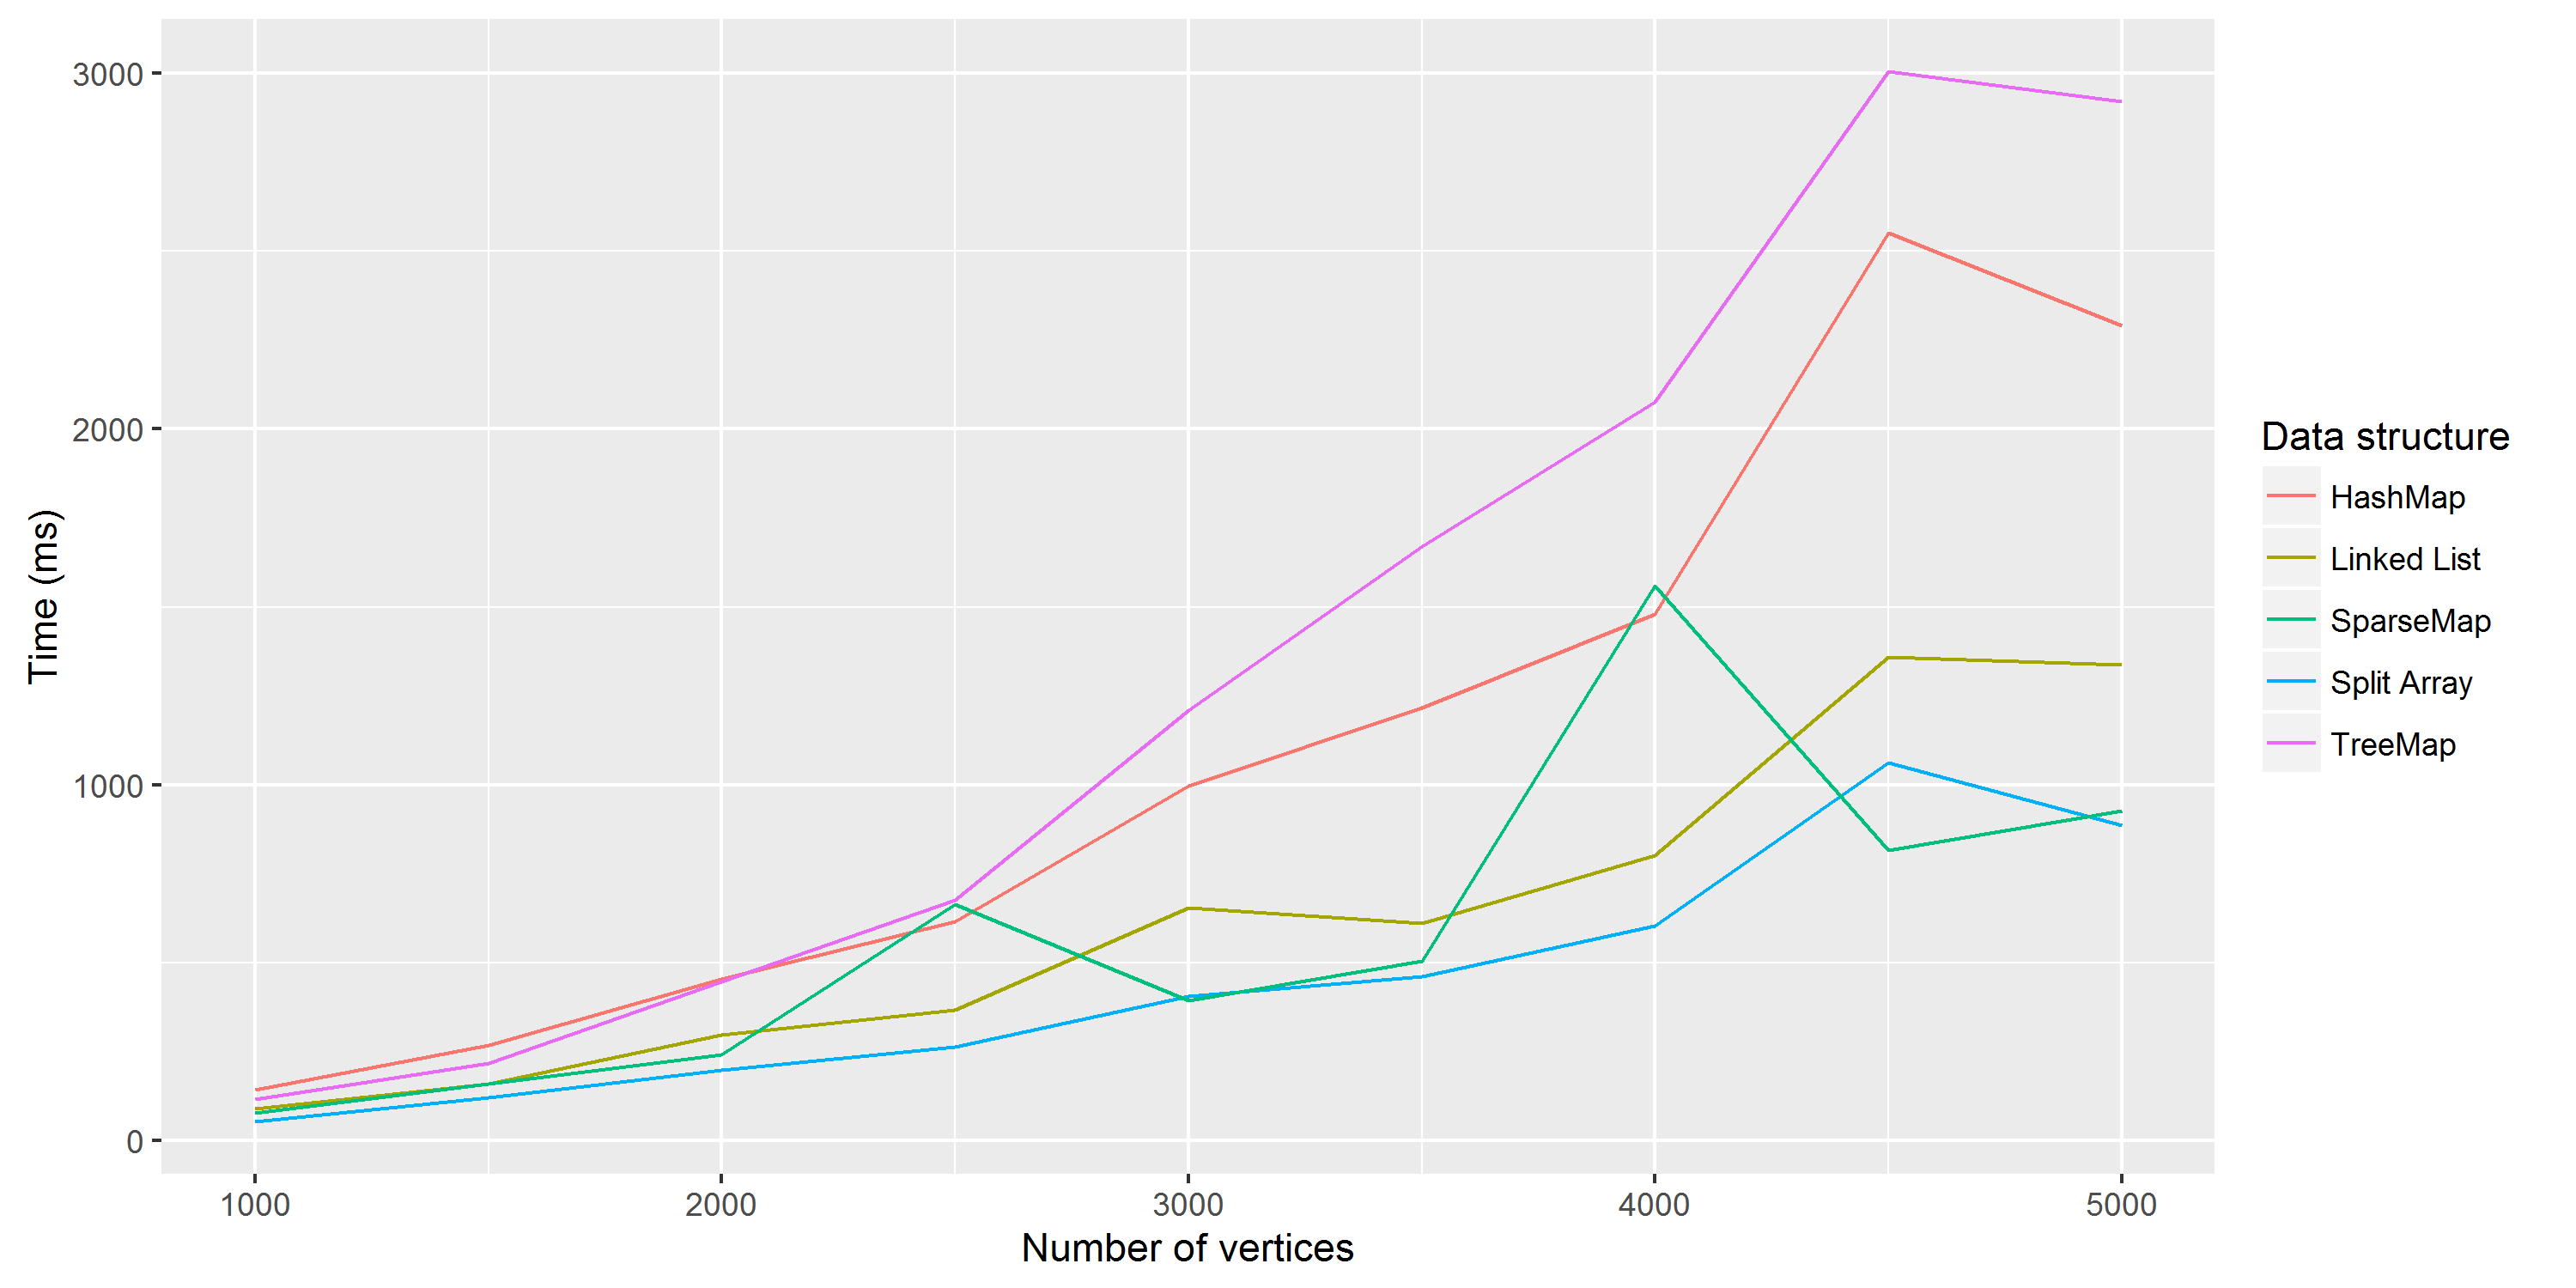
\includegraphics[scale=0.5]{images/results/ekmeansize.png}
\caption{Average run time of all data structures with Edmonds-Karp on size variation instances.}
\label{fig:ekmeansize}
\end{center}
\end{figure}
\begin{figure}[H]
\begin{center}
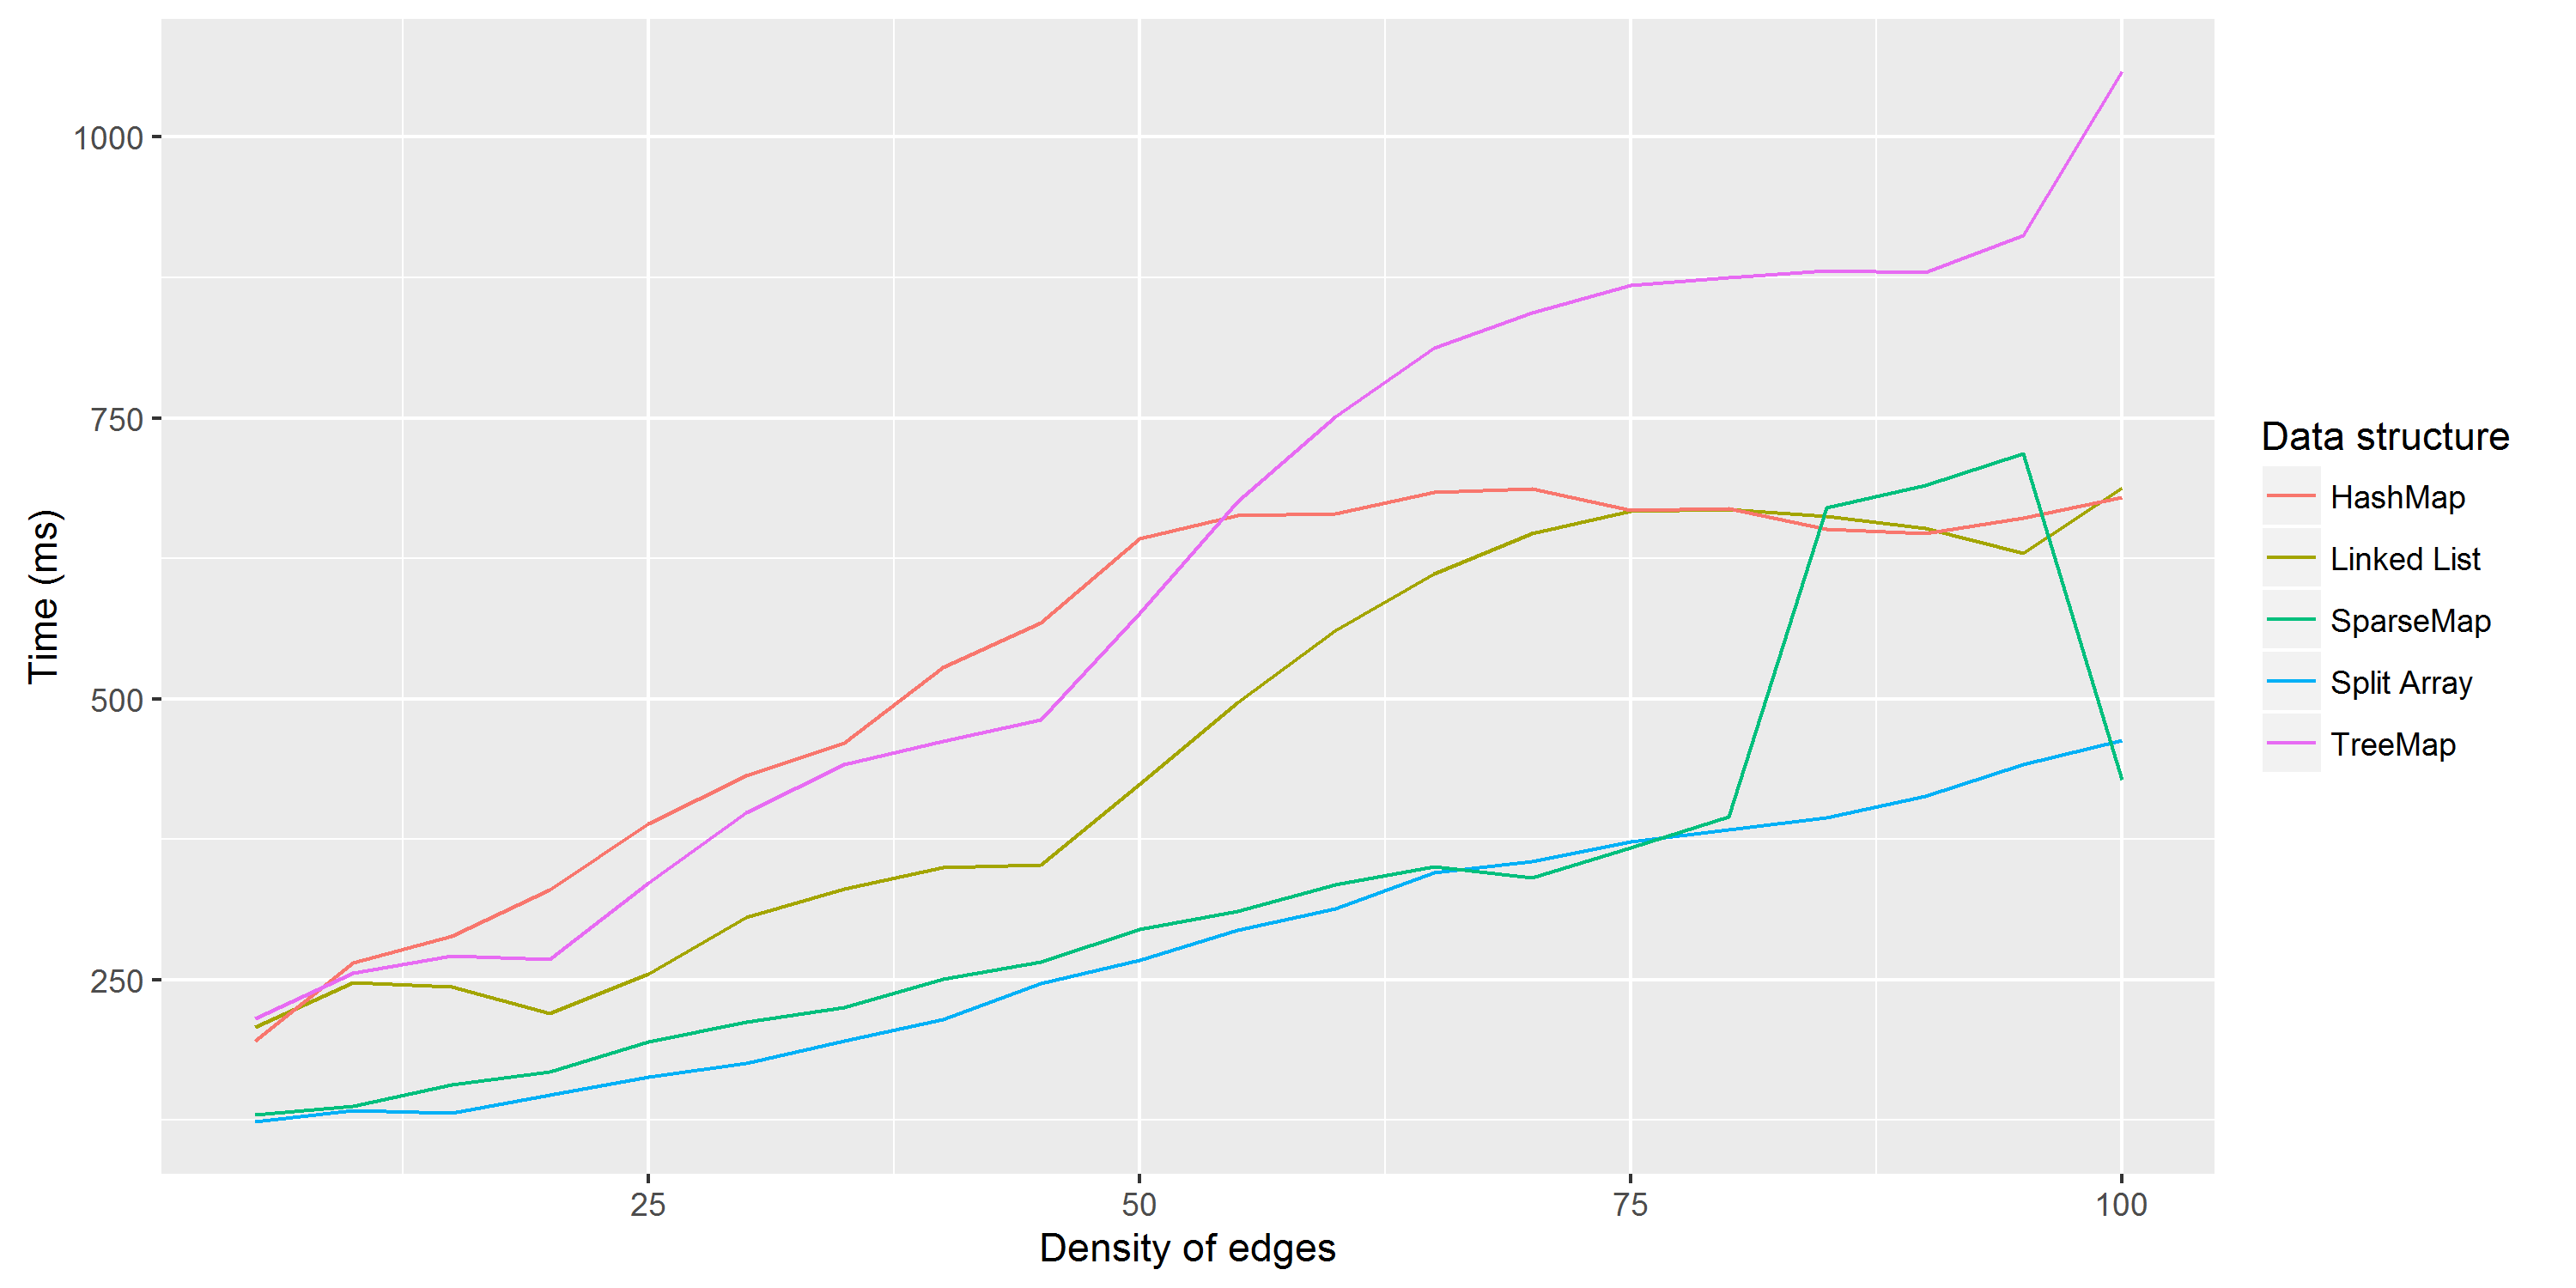
\includegraphics[scale=0.5]{images/results/ekmeanmatching.png}
\caption{Average run time of all data structures with Edmonds-Karp on matching instances.}
\label{fig:ekmeanmatching}
\end{center}
\end{figure}
As we can see, the data structures based on the $sparse set$ provide better performances than the others. The $hash map$ and $tree map$ are the least efficient. We can conclude that the most appropriate data structure for Edmonds-Karp is the $split array$.
\subsection{Ford-Fulkerson with scaling}
The Figure \ref{fig:ffmeandensity}, \ref{fig:ffmeansize} and \ref{fig:ffmeanmatching} represents the average run time of all data structures with Ford-Fulkerson with scaling. They were computed on, respectively, the density variation, the size variation and the matching instances.
\begin{figure}[H]
\begin{center}
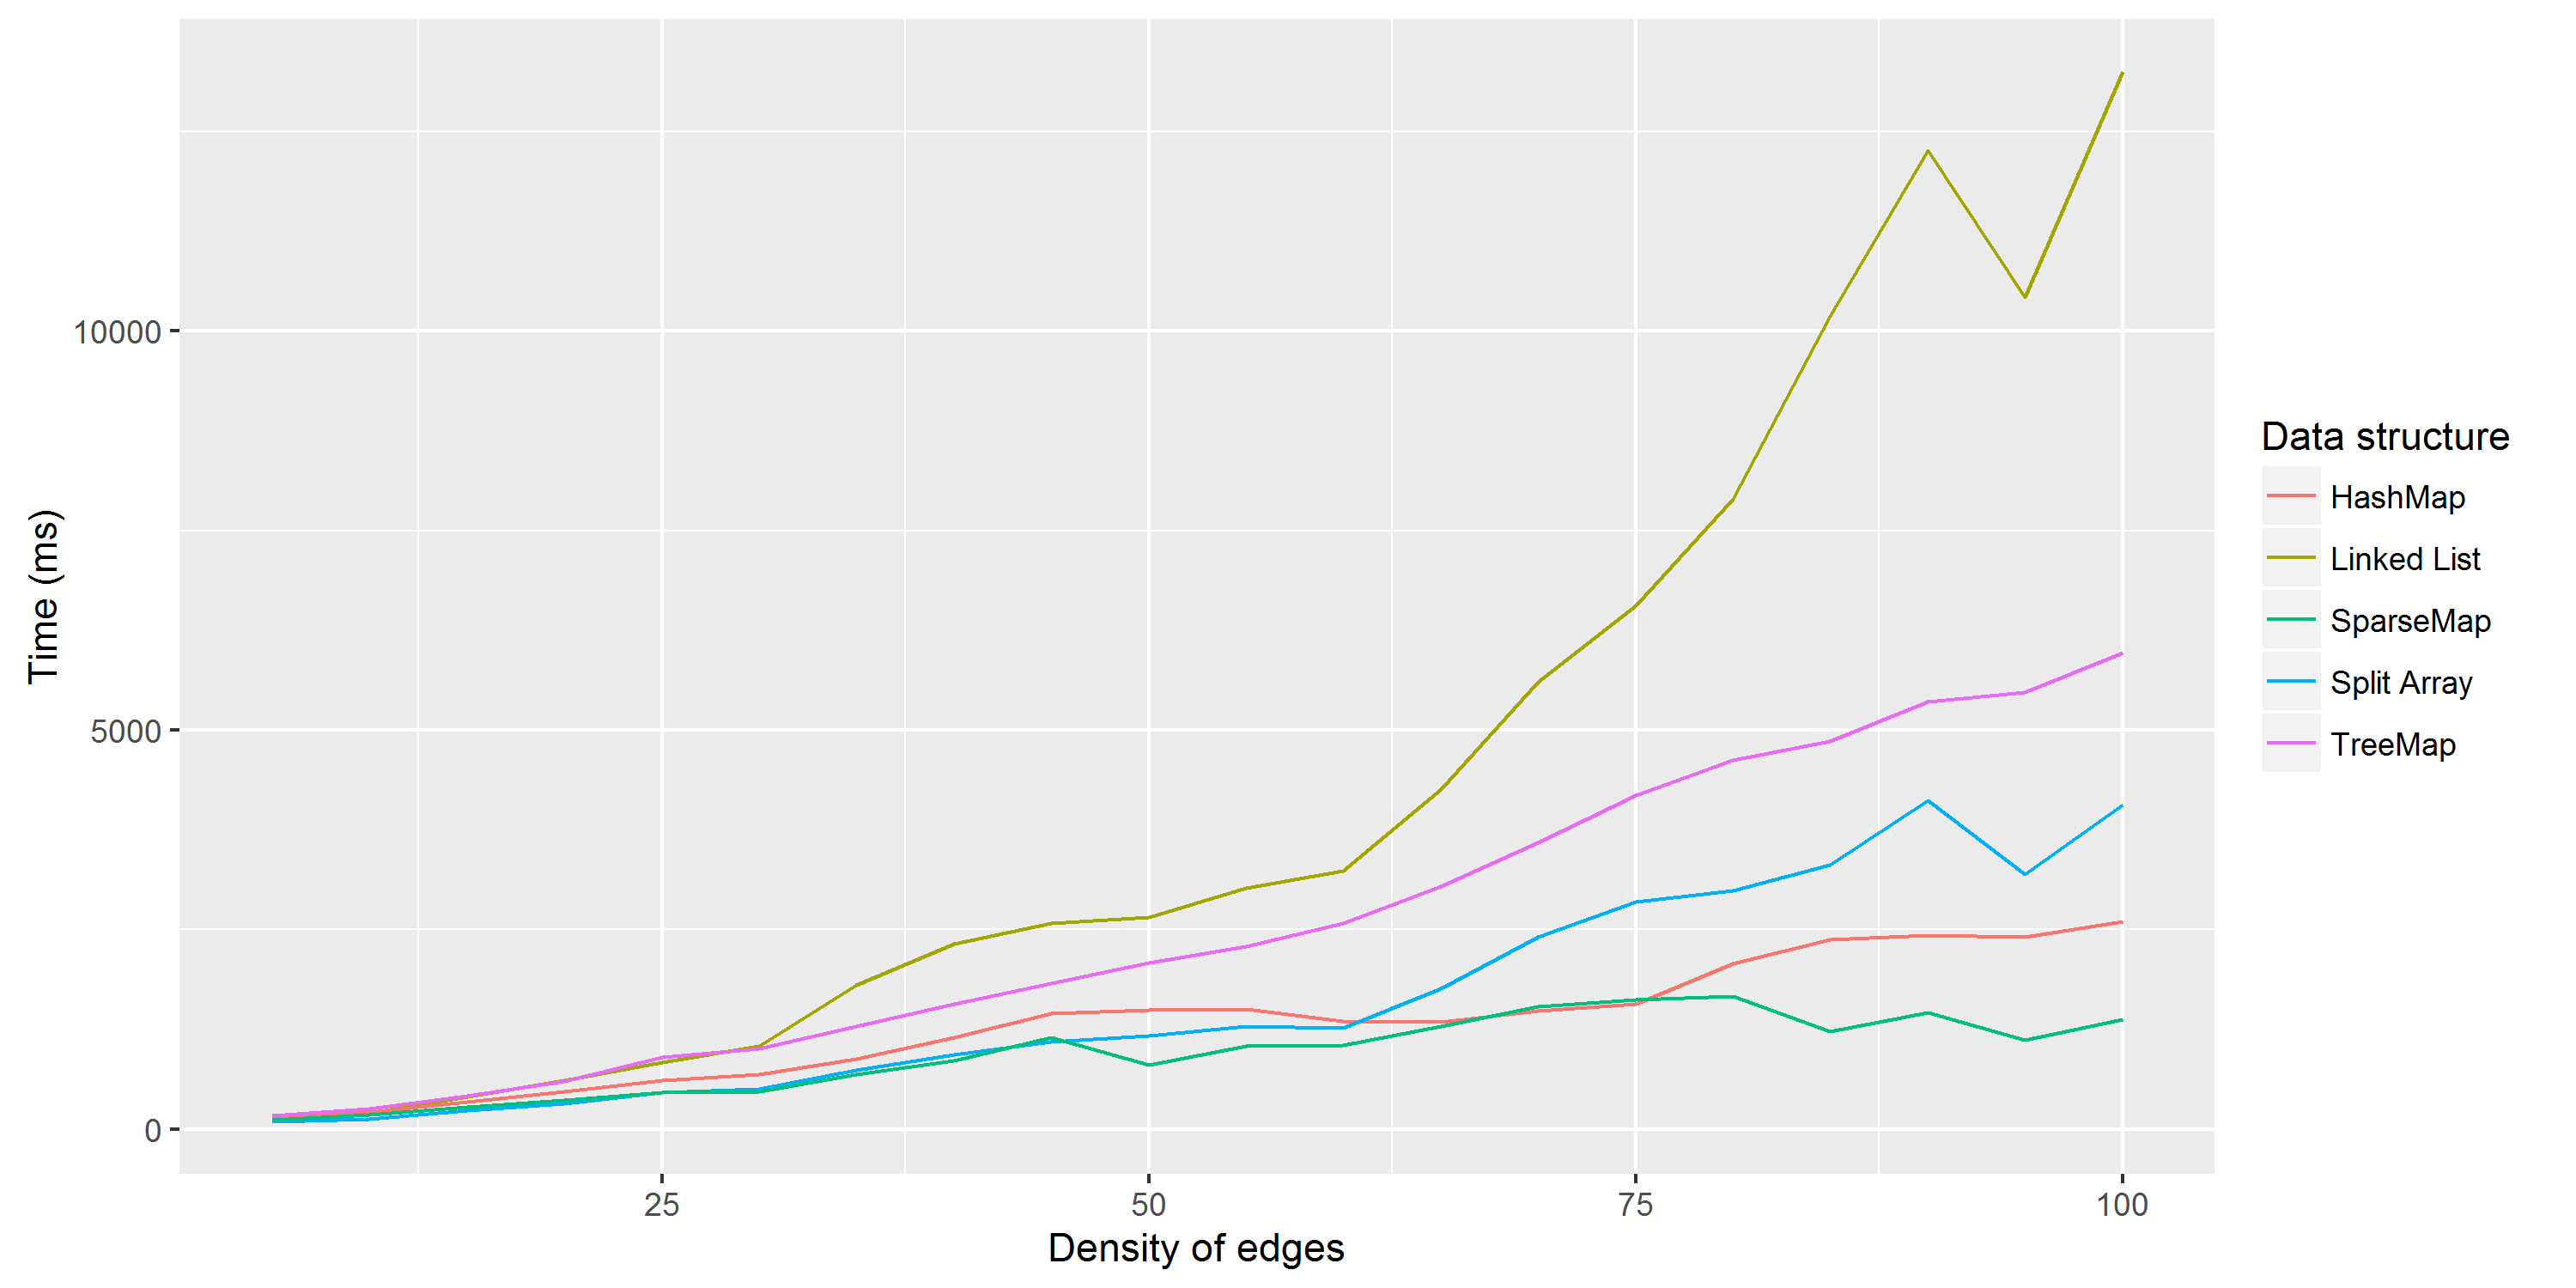
\includegraphics[scale=0.5]{images/results/ffmeandensity.png}
\caption{Average run time of all data structures with Ford-Fulkerson with scaling on density variation instances.}
\label{fig:ffmeandensity}
\end{center}
\end{figure}
\begin{figure}[H]
\begin{center}
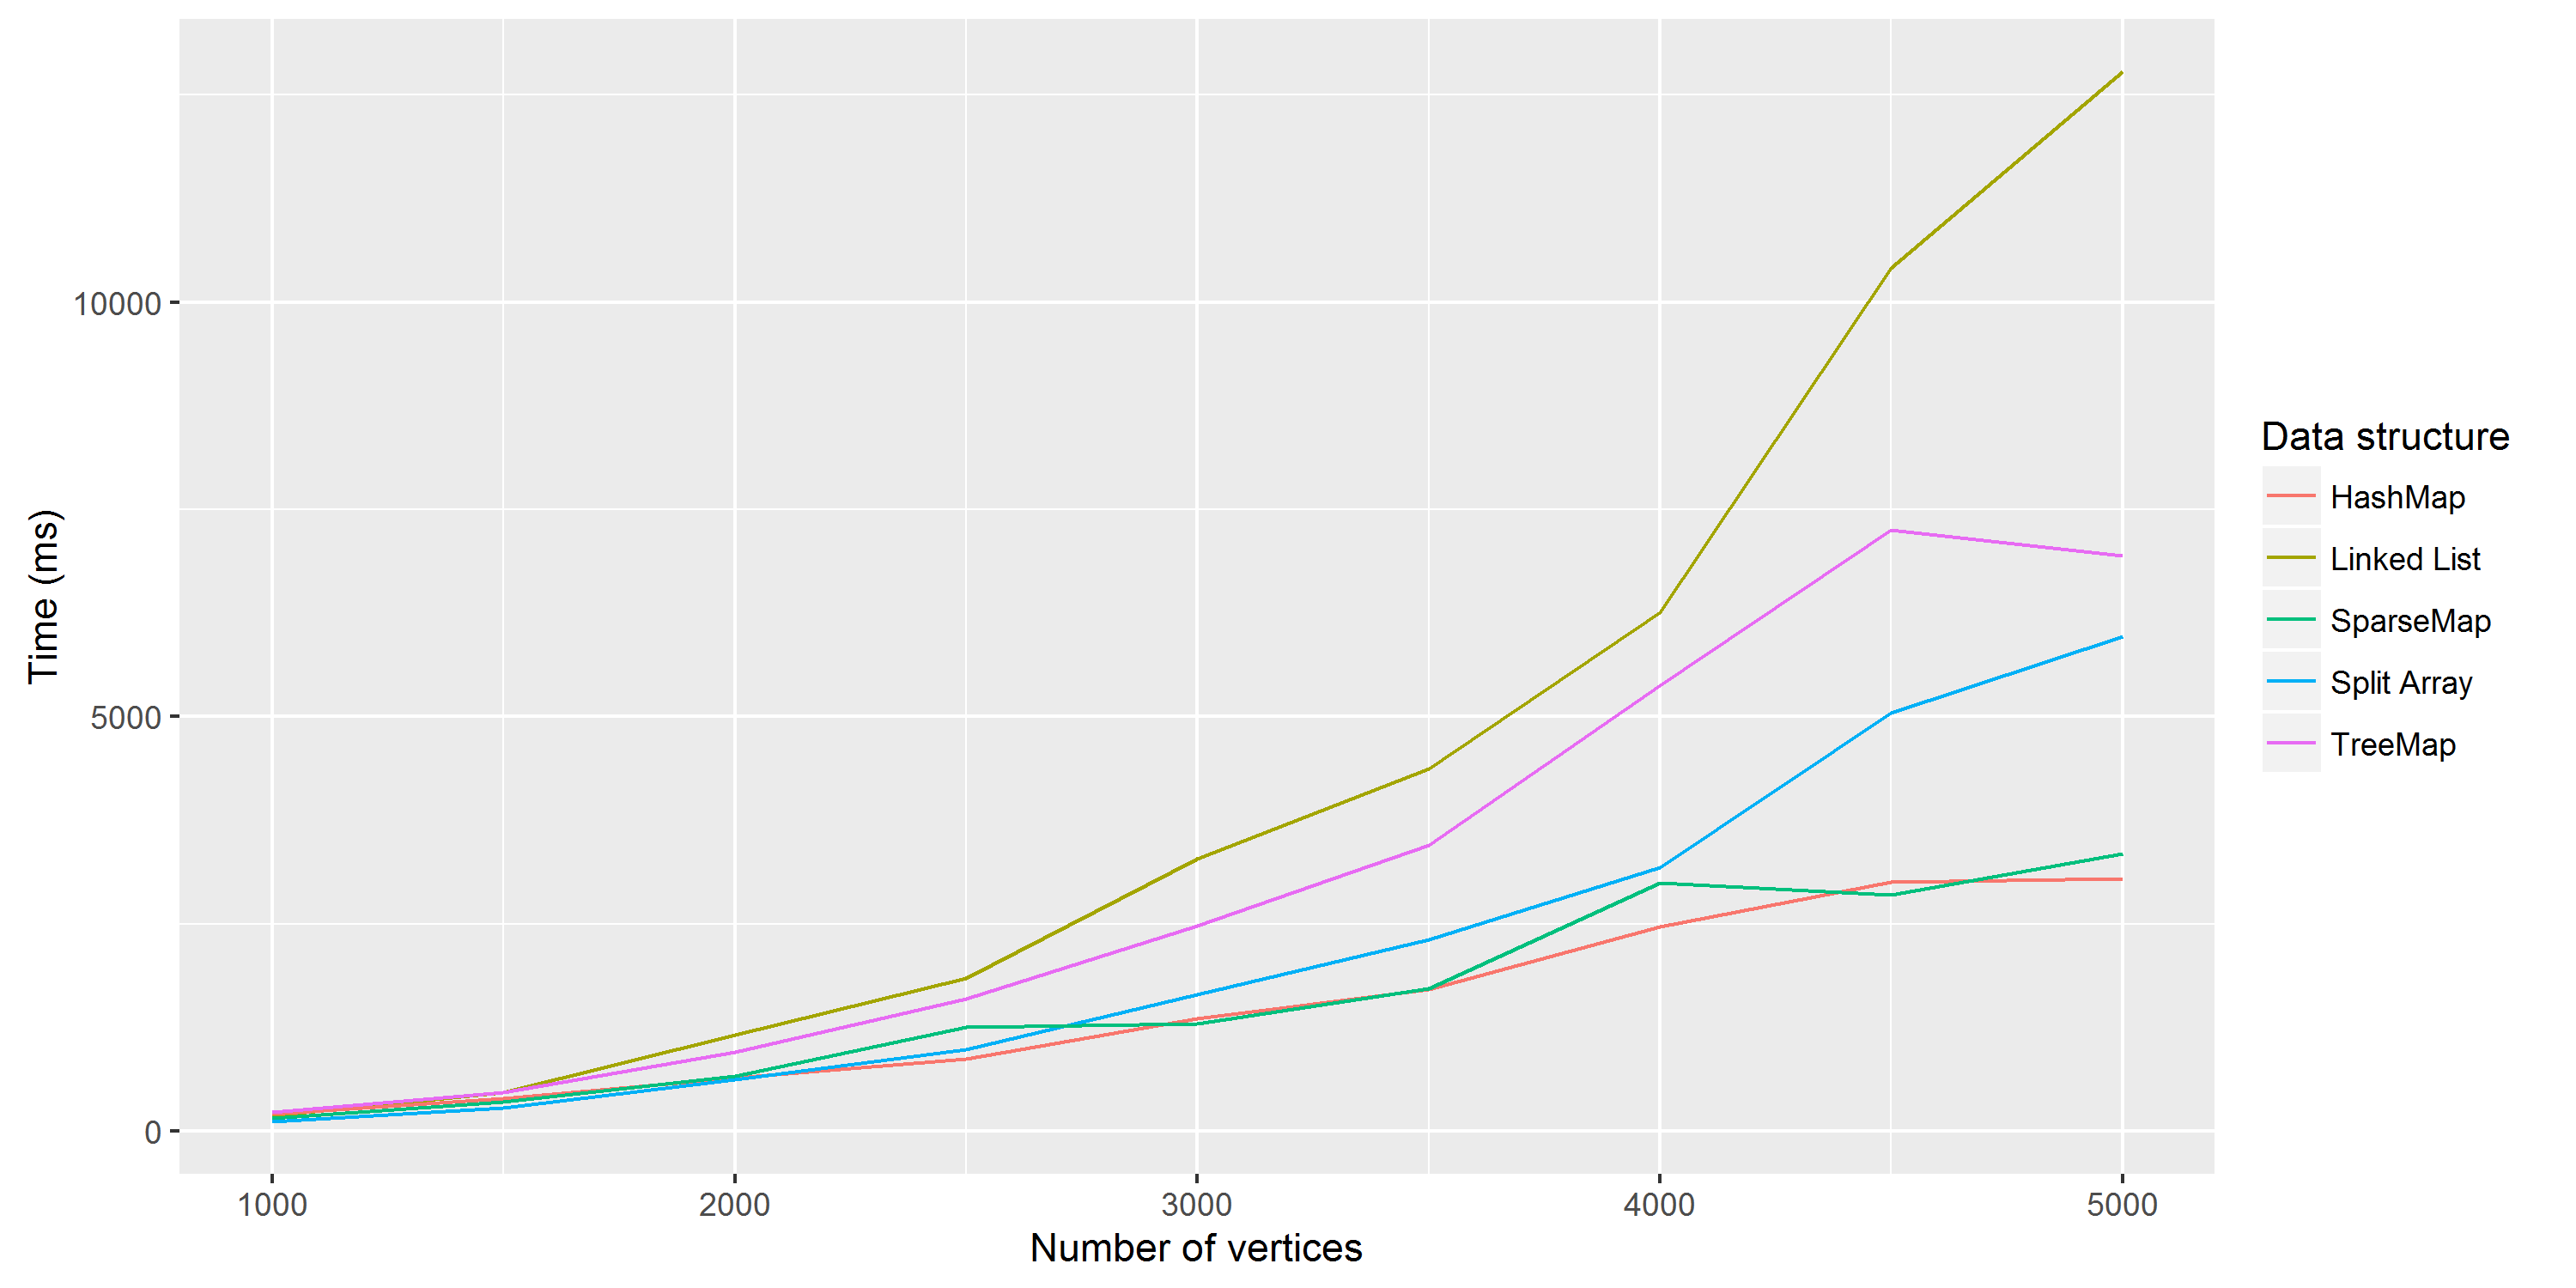
\includegraphics[scale=0.5]{images/results/ffmeansize.png}
\caption{Average run time of all data structures with Ford-Fulkerson with scaling on size variation instances.}
\label{fig:ffmeansize}
\end{center}
\end{figure}
\begin{figure}[H]
\begin{center}
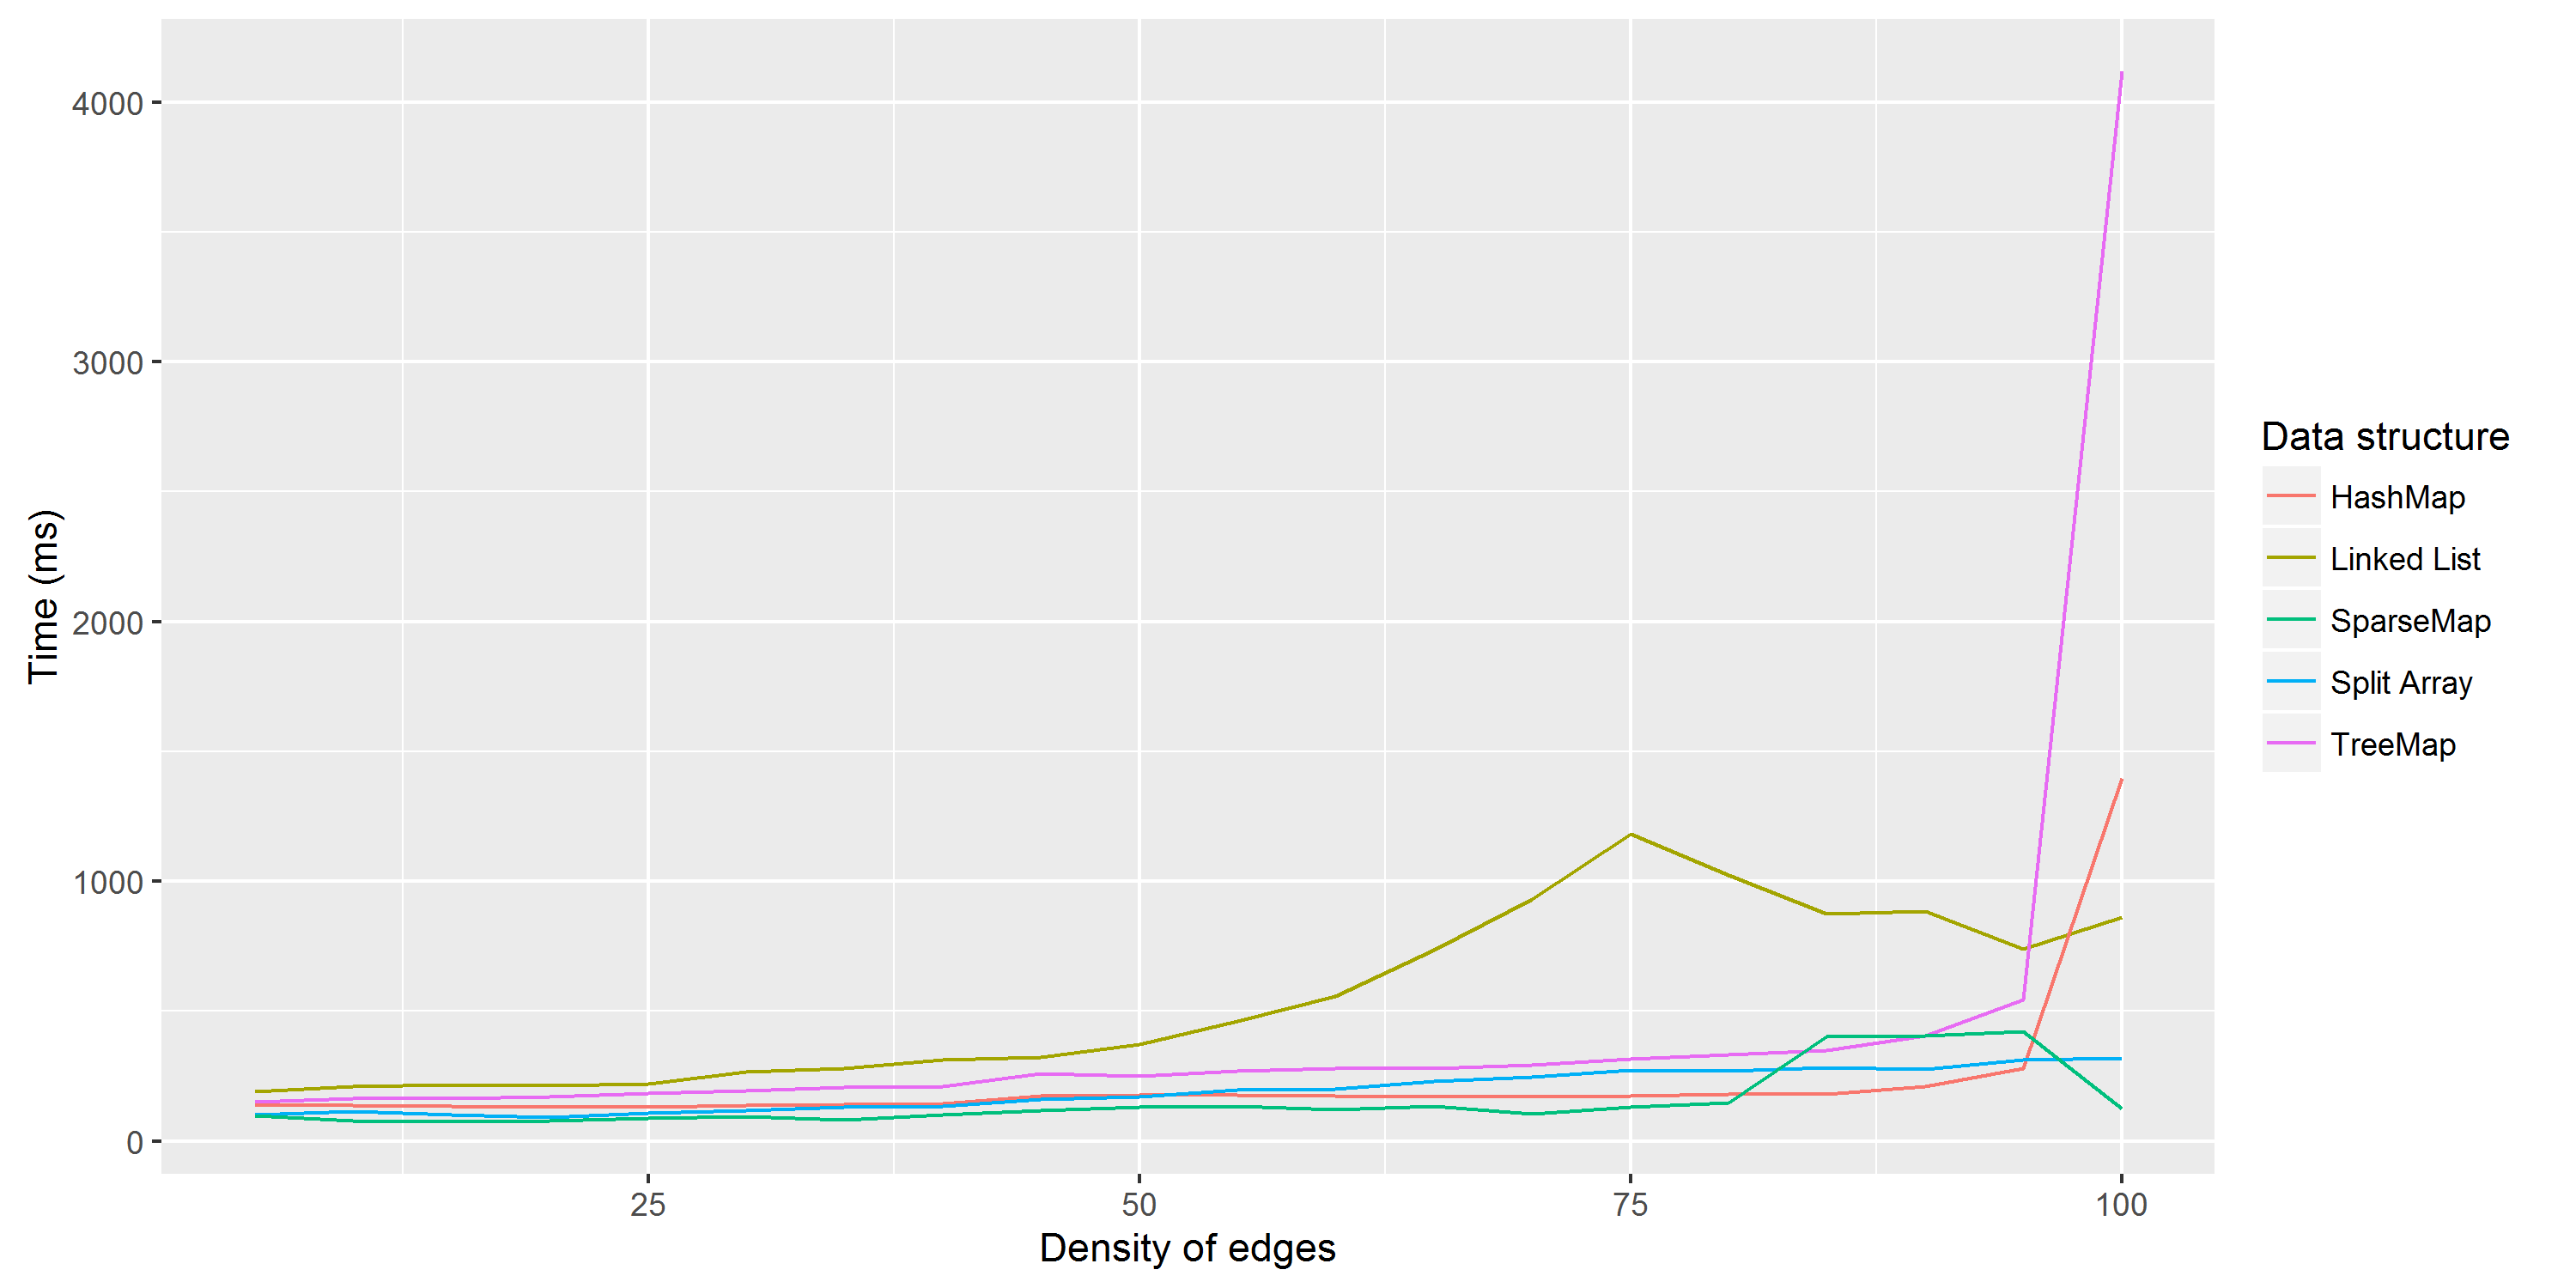
\includegraphics[scale=0.5]{images/results/ffmeanmatching.png}
\caption{Average run time of all data structures with Ford-Fulkerson with scaling on matching instances.}
\label{fig:ffmeanmatching}
\end{center}
\end{figure}
Those figures highlight the poor performance of the $linked list$ while the $sparsemap$ seems to be the most appropriate data structure for Ford-Fulkerson with scaling.
\section{Behaviors}
\subsection{Edmonds-Karp}
\subsubsection{Density variation instances}
One of the most blatant observations on Edmonds-Karp is that it is very regular, what we can observe in the Figure~\ref{fig:EKmean}, which represents the run time on each density variation instance, with its best data structure, the $split array$. Indeed, Edmonds-Karp solve the maximum flow problem on complete graphs with $|V|=1000$ with a run time ranging from 750 to 1000 ms.
\begin{figure}[H]
\begin{center}
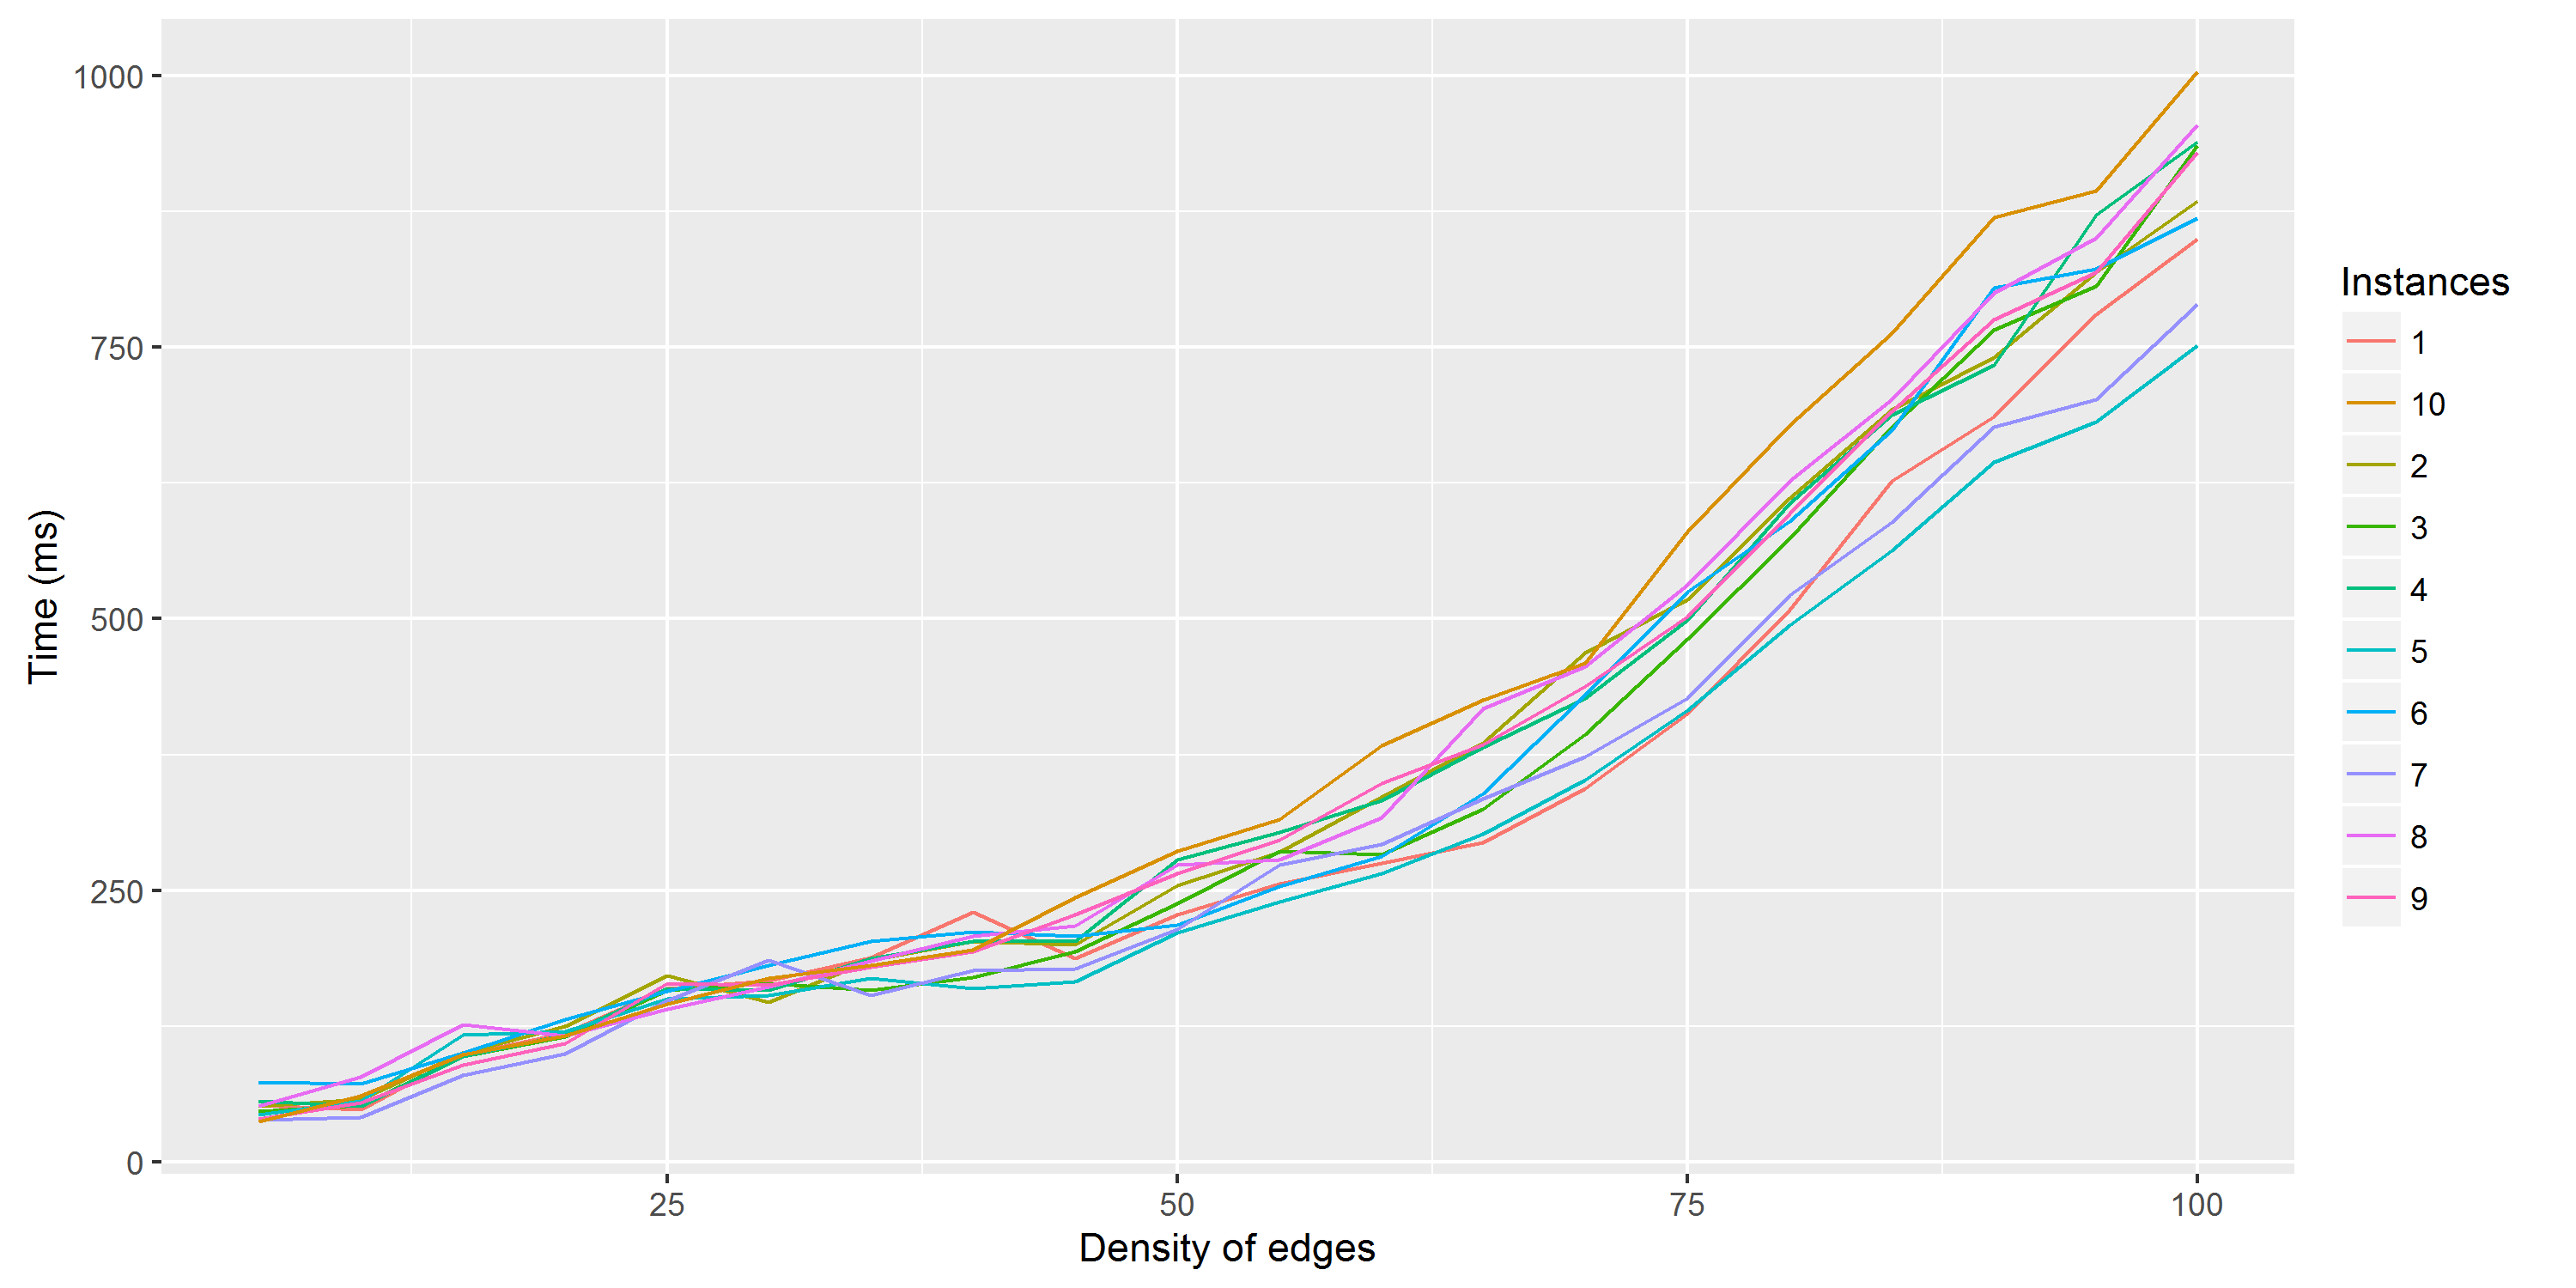
\includegraphics[scale=0.5]{images/results/EKmean.png}
\caption{Run time of Edmonds-Karp on all density variation instances with the $split array$.}
\label{fig:EKmean}
\end{center}
\end{figure}
\subsubsection{Size variation instances}
The Figure~\ref{fig:EKmeansize} represents the run time of Edmonds-Karp on all size variation instances with the $split array$. Edmonds-Karp is regular with a run time ranging from 750 to 1000 ms to solve the maximum flow problem on graphs with $|V|=5000$ and a density of edges equal to 10\% ($|E|=1249750$).
\begin{figure}[H]
\begin{center}
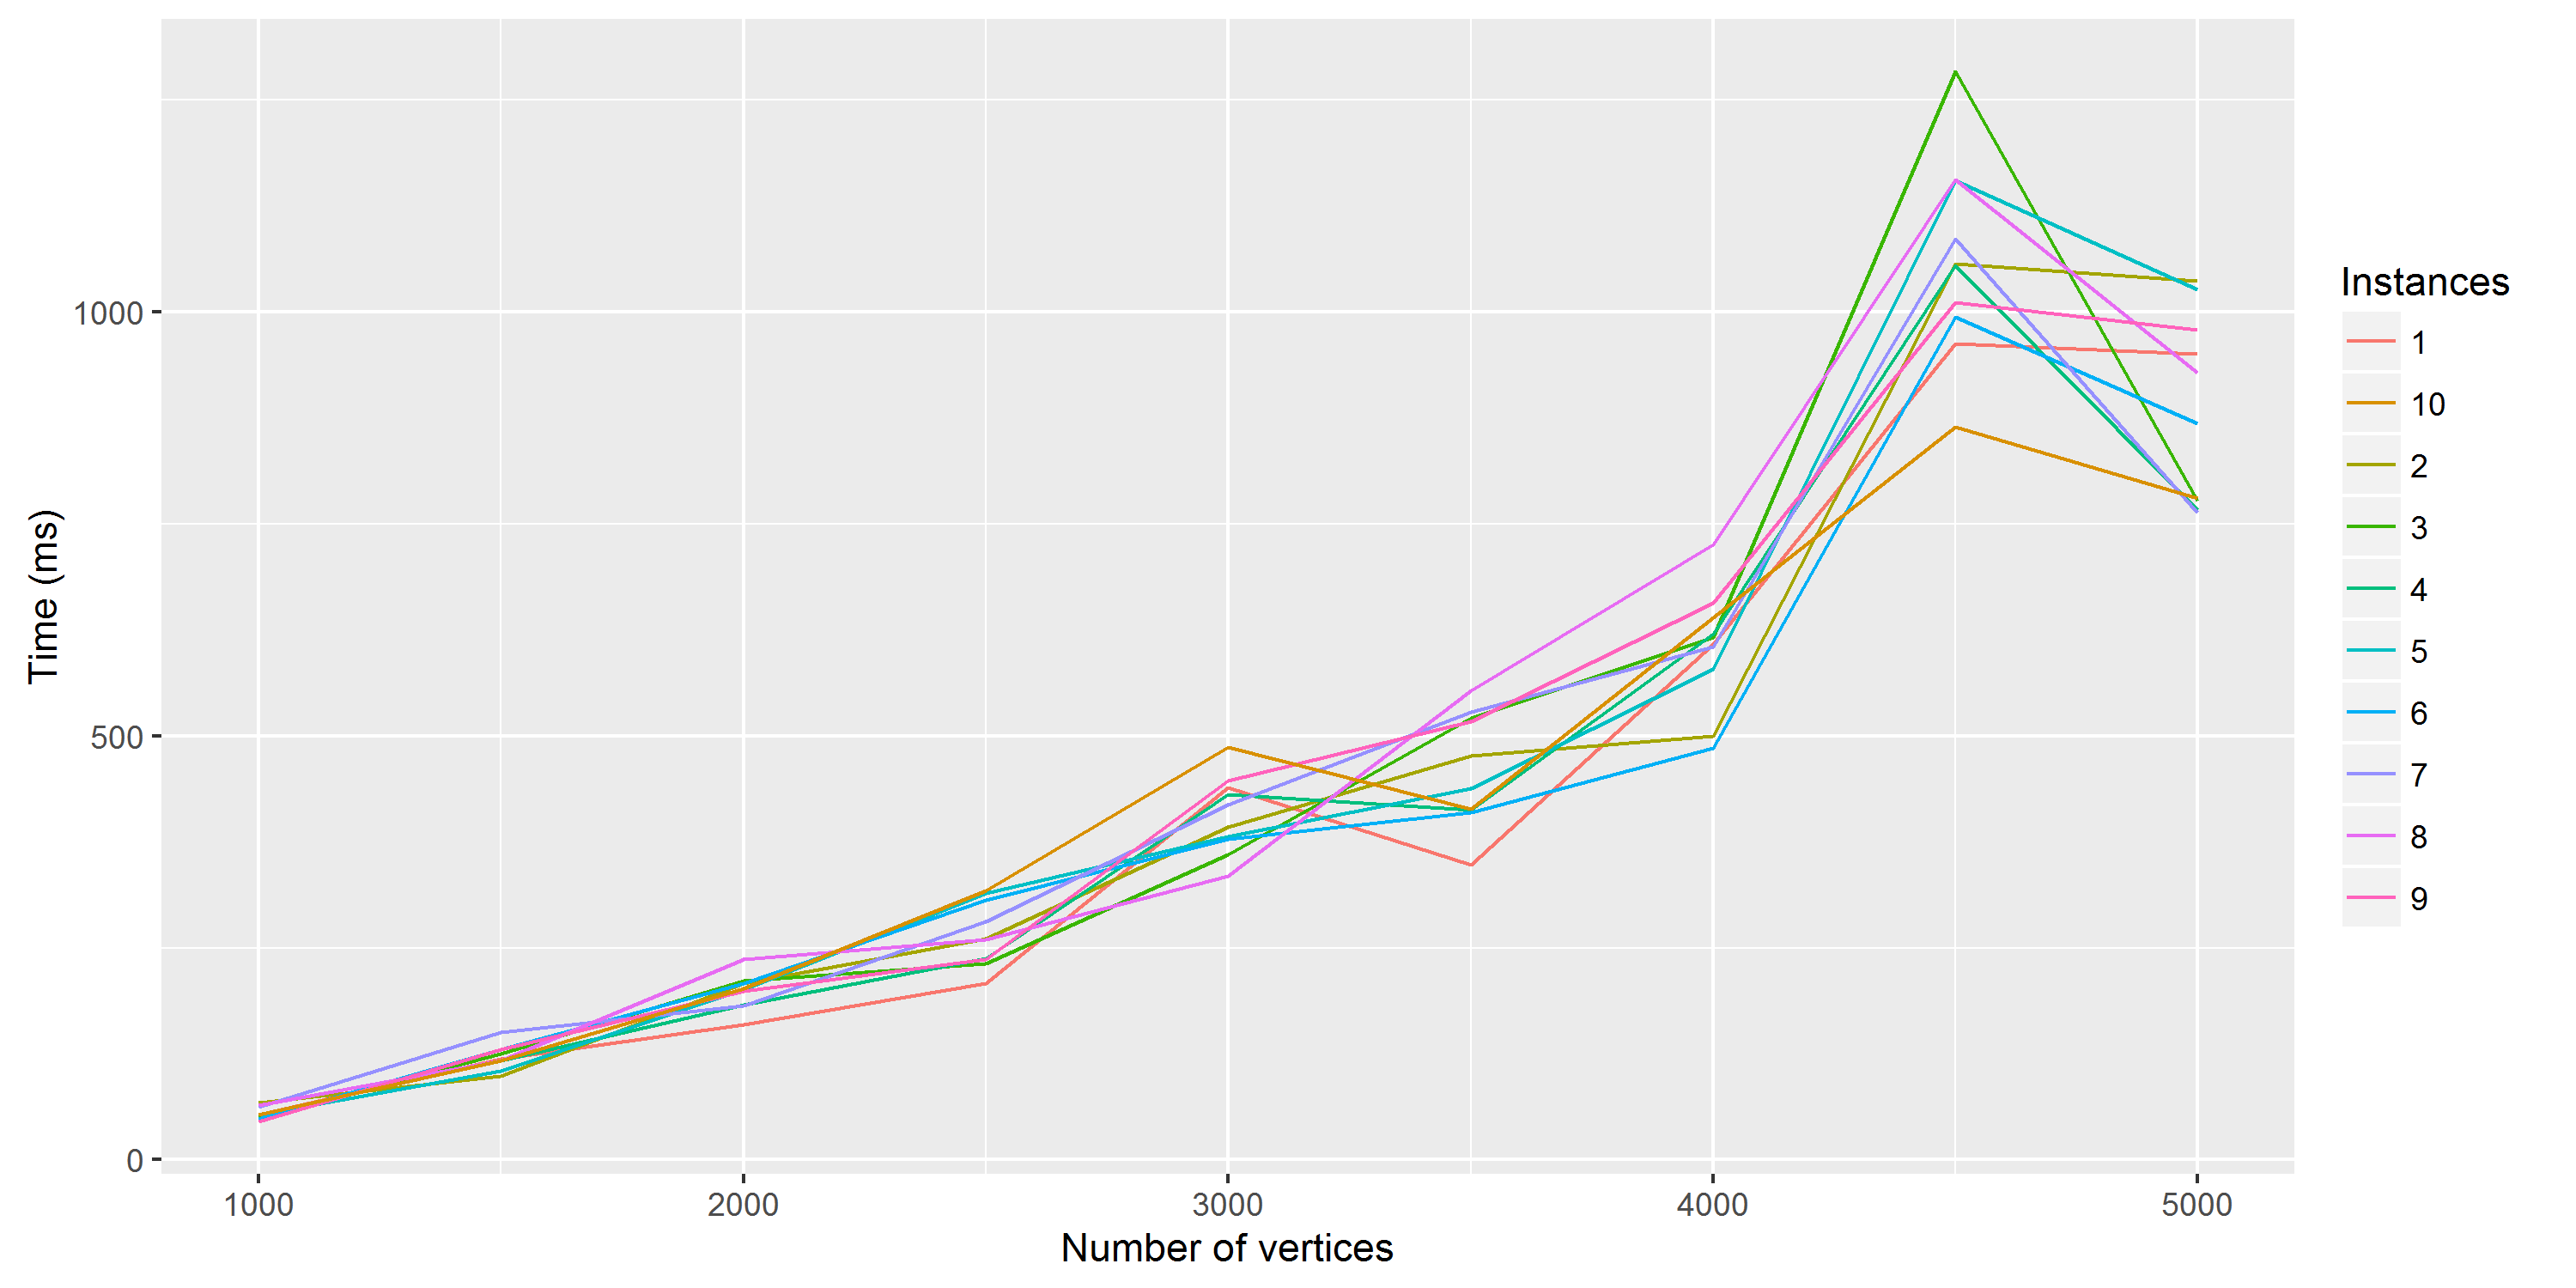
\includegraphics[scale=0.5]{images/results/EKmeansize2.png}
\caption{Run time of Edmonds-Karp on all size variation instances with the $split array$.}
\label{fig:EKmeansize}
\end{center}
\end{figure}
\subsubsection{Matching instances}
As usual, Edmonds-Karp remains very regular. We can see that on the Figure~\ref{fig:ekmatching} which represents the run time of Edmonds-Karp on all matching instances. It takes an average of 460ms to solve a matching instance with a maximum density of edges.
\begin{figure}[H]
\begin{center}
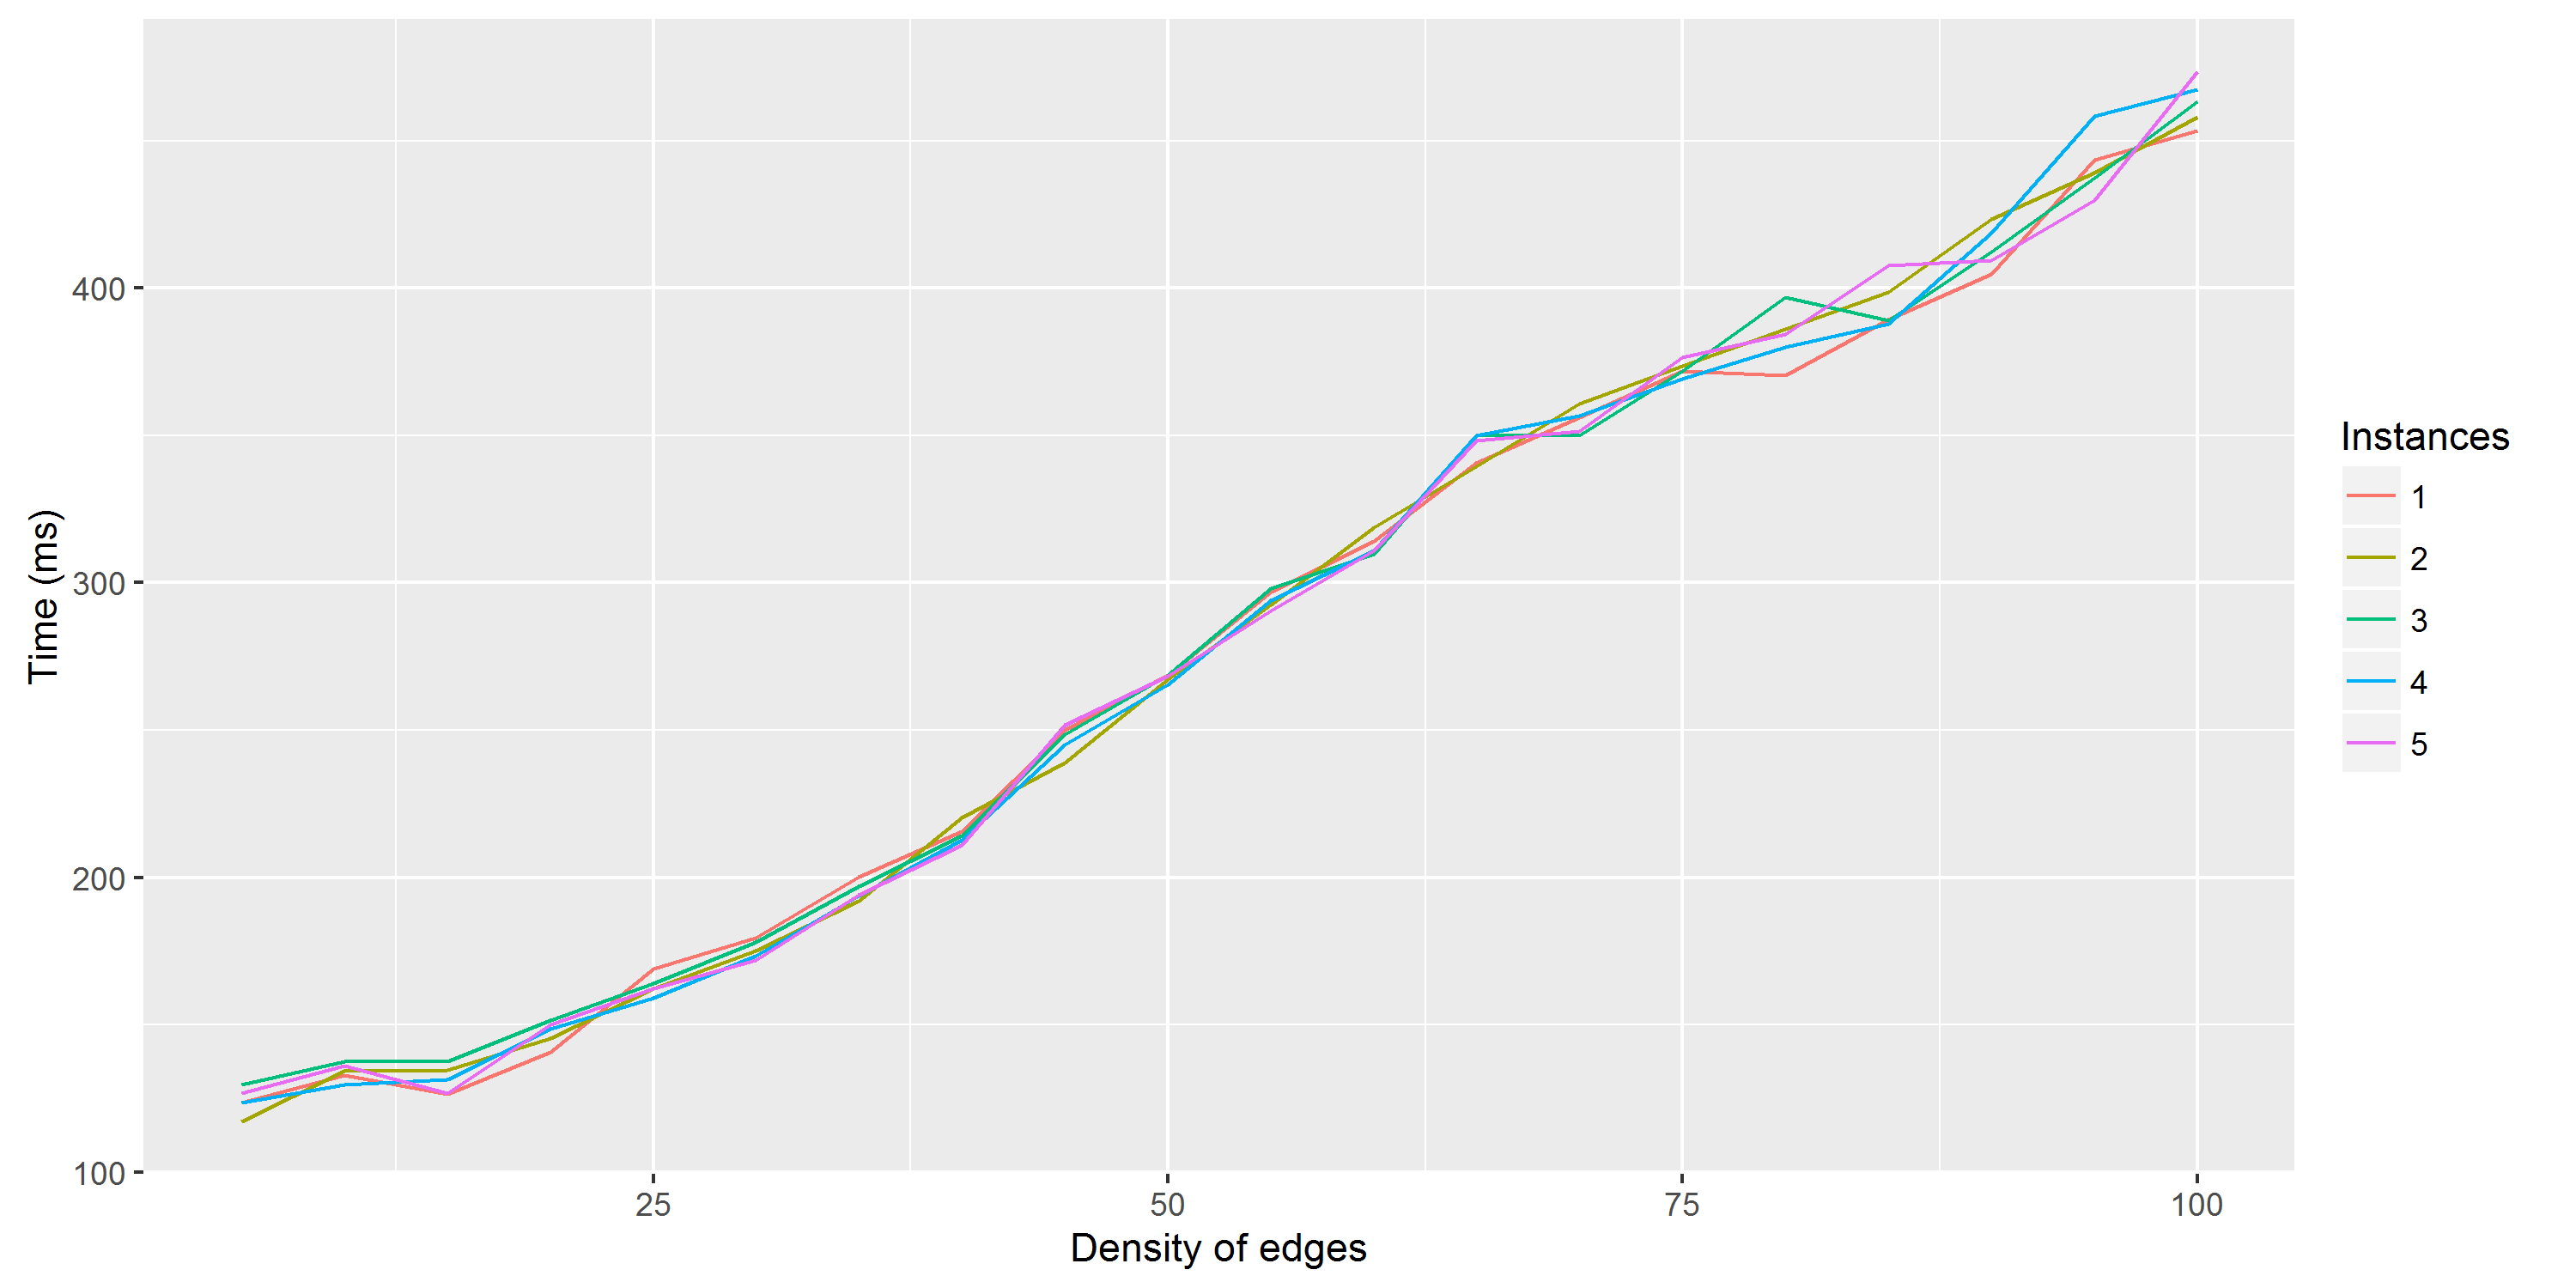
\includegraphics[scale=0.5]{images/results/ekmatching.png}
\caption{Run time of Edmonds-Karp on all matching instances with the $split array$.}
\label{fig:ekmatching}
\end{center}
\end{figure}
\subsection{Ford-Fulkerson with scaling}
\subsubsection{Density variation instances}
The Figure~\ref{fig:FFmean} represents the run time on each density variation instance, with the $sparsema$p. Although less regular than Edmonds-Karp, Ford-Fulkerson with scaling remains stable with a run time ranging from 500 to 2500 ms to solve the maximum flow problem on complete graphs with $|V|=1000$.
\begin{figure}[H]
\begin{center}
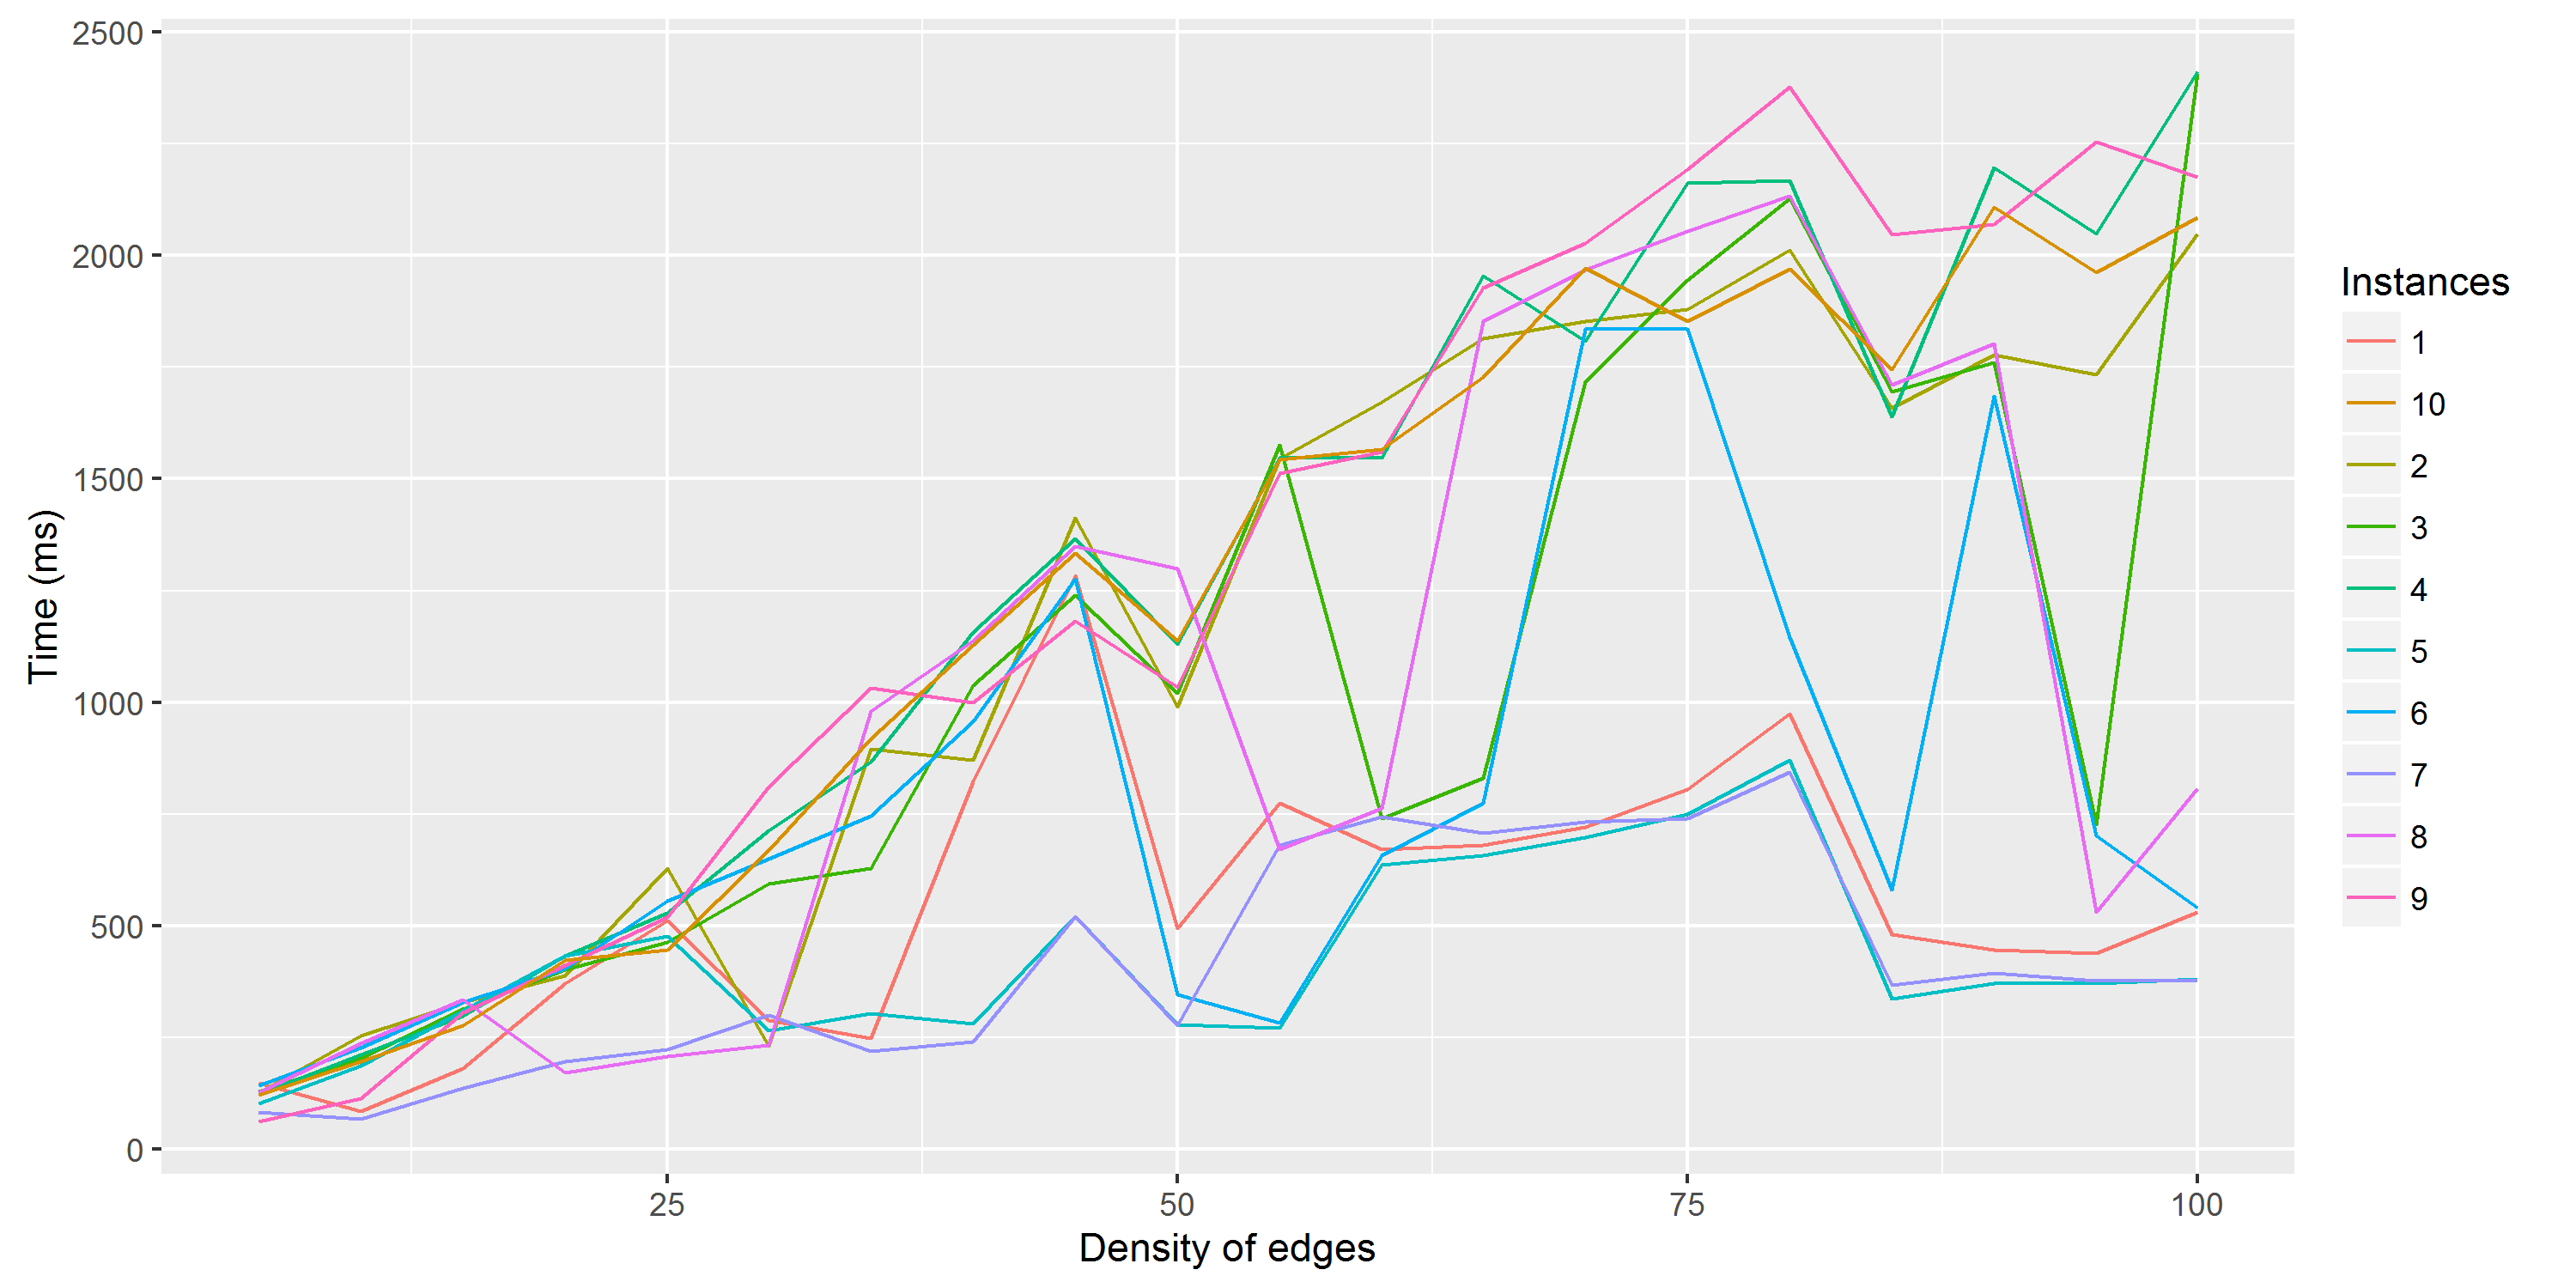
\includegraphics[scale=0.5]{images/results/FFmean.png}
\caption{Run time of Ford-Fulkerson with scaling on all density variation instances with the $sparse map$.}
\label{fig:FFmean}
\end{center}
\end{figure}
\subsubsection{Size variation instances}
As we can see on the Figure~\ref{fig:FFmeansize} which represents the run time of Ford-Fulkerson with scaling on all size variation instances, it is quite regular but its performances are slightly worse than Edmonds-Karp. Indeed, Ford-Fulkerson with scaling solve the maximum flow problem on graphs with $|V|=5000$ and a density of edges equal to 10\% with a run time ranging from 3000 to 4000 ms.
\begin{figure}[H]
\begin{center}
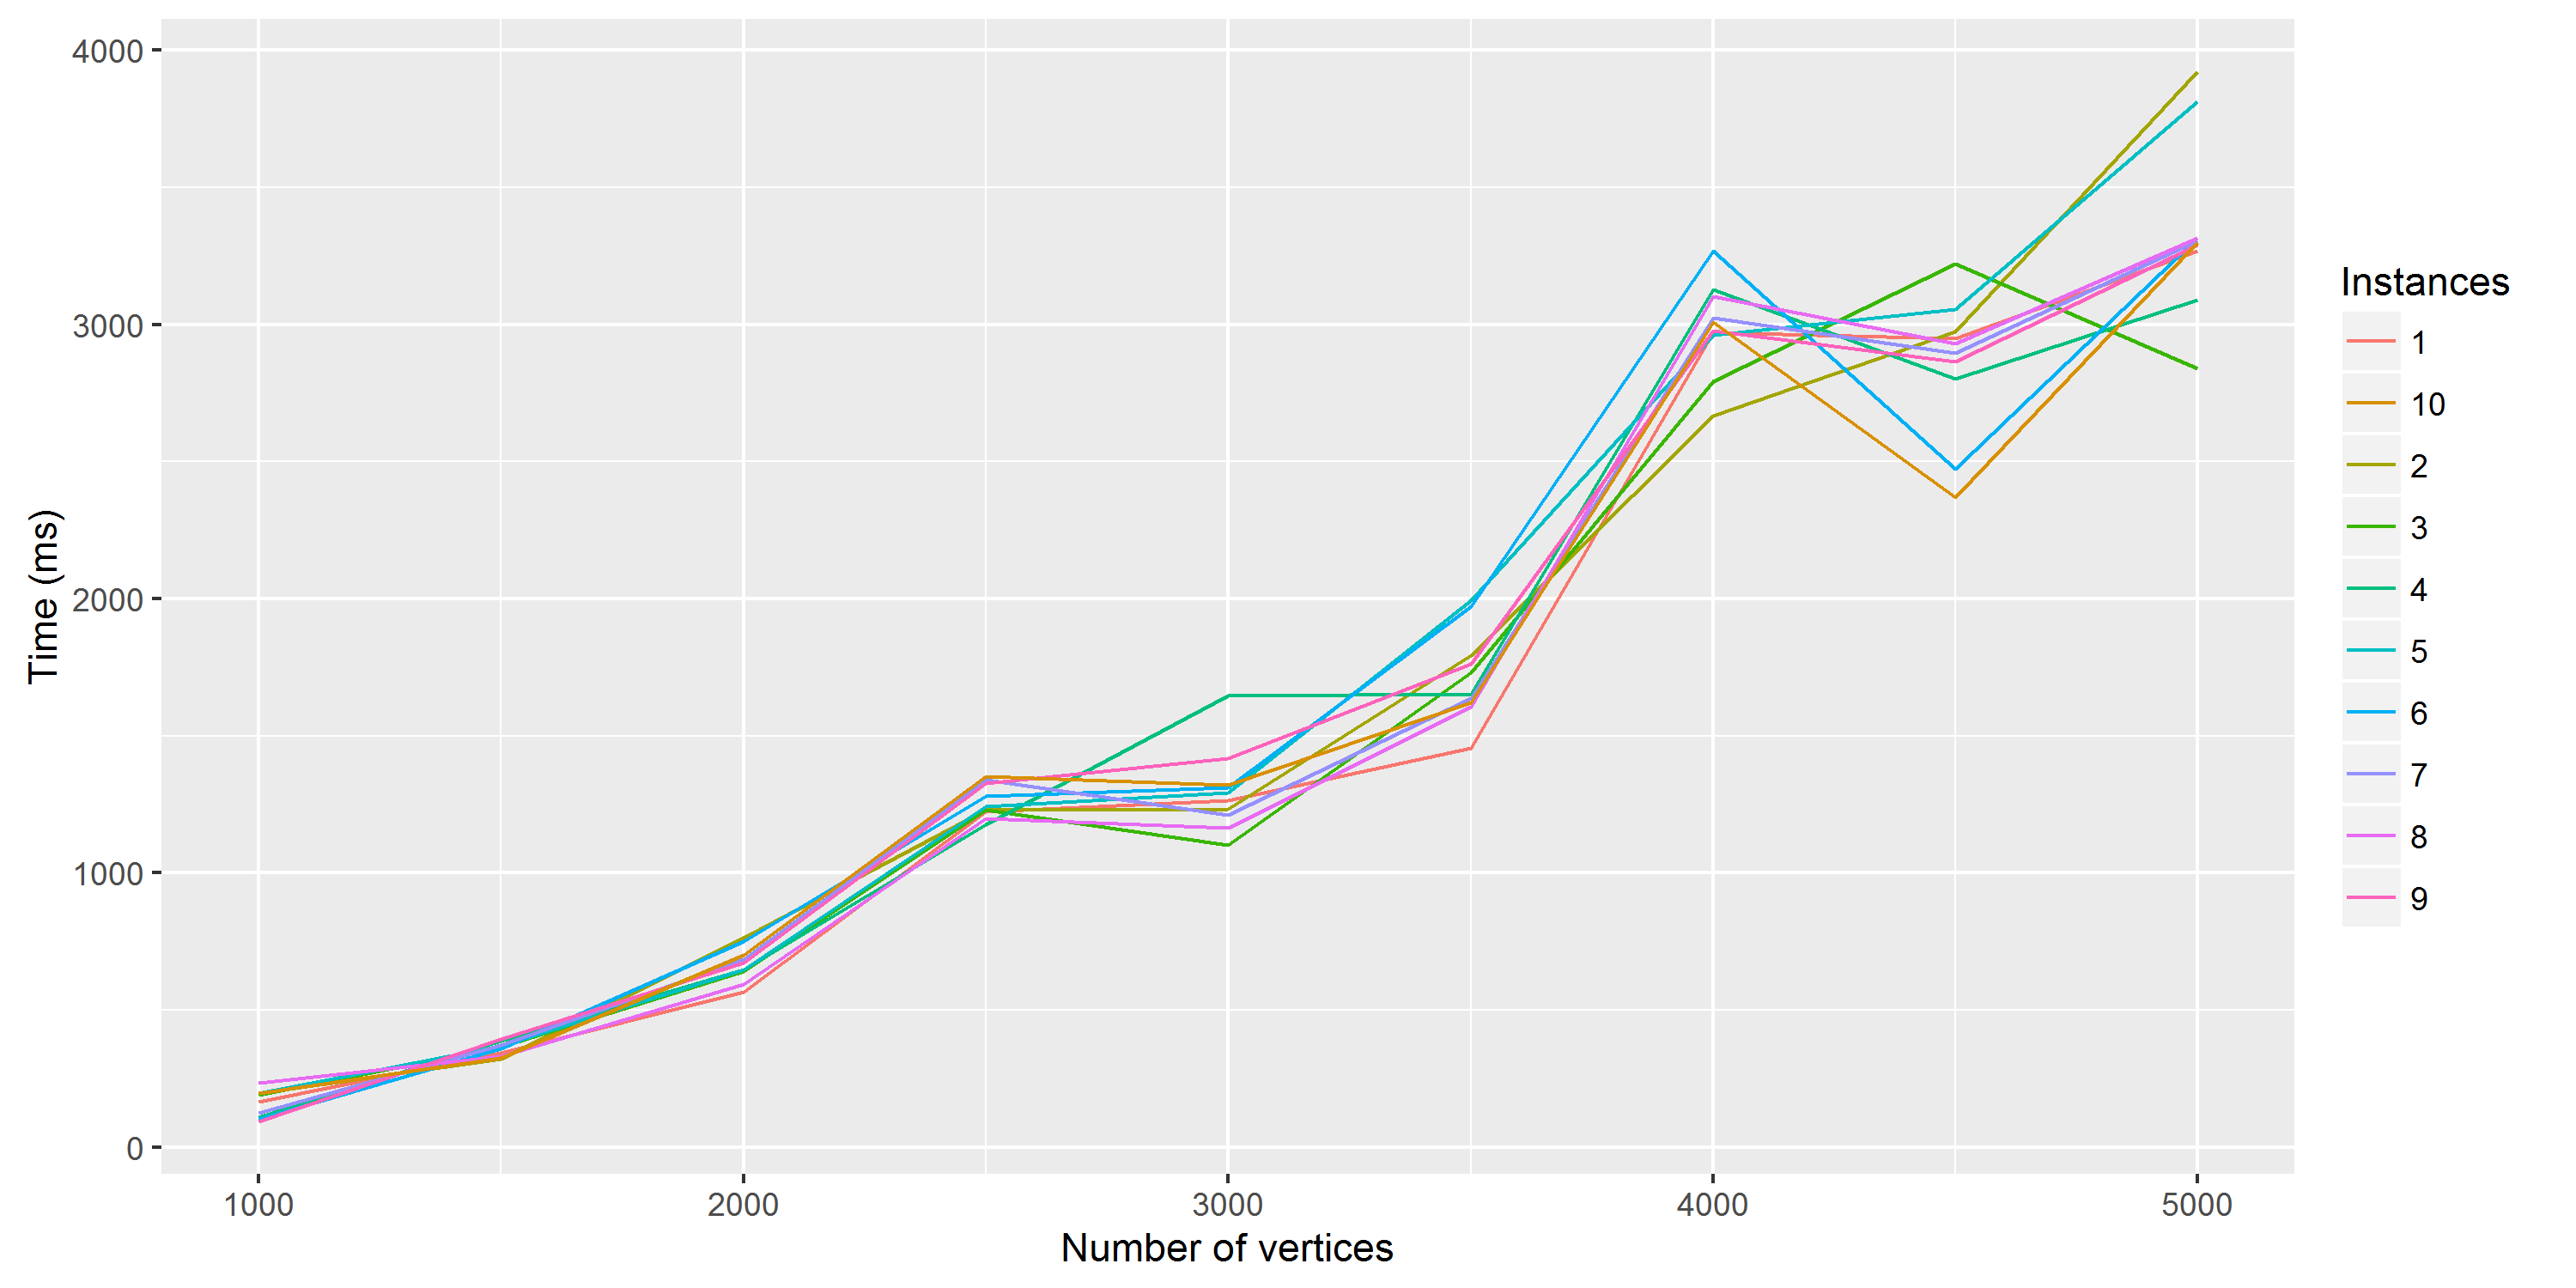
\includegraphics[scale=0.5]{images/results/FFmeansize2.png}
\caption{Run time of Ford-Fulkerson with scaling on all size variation instances with the $sparse map$.}
\label{fig:FFmeansize}
\end{center}
\end{figure}
\subsubsection{Matching instances}
The Figure~\ref{fig:ffmatching} show that Ford-Fulkerson with scaling has a constant run time to solve this kind of instance. The pike present at the end of the graph is due to its data structure. It takes an average of 120ms to solve a matching instance with a maximum density of edges.
\begin{figure}[H]
\begin{center}
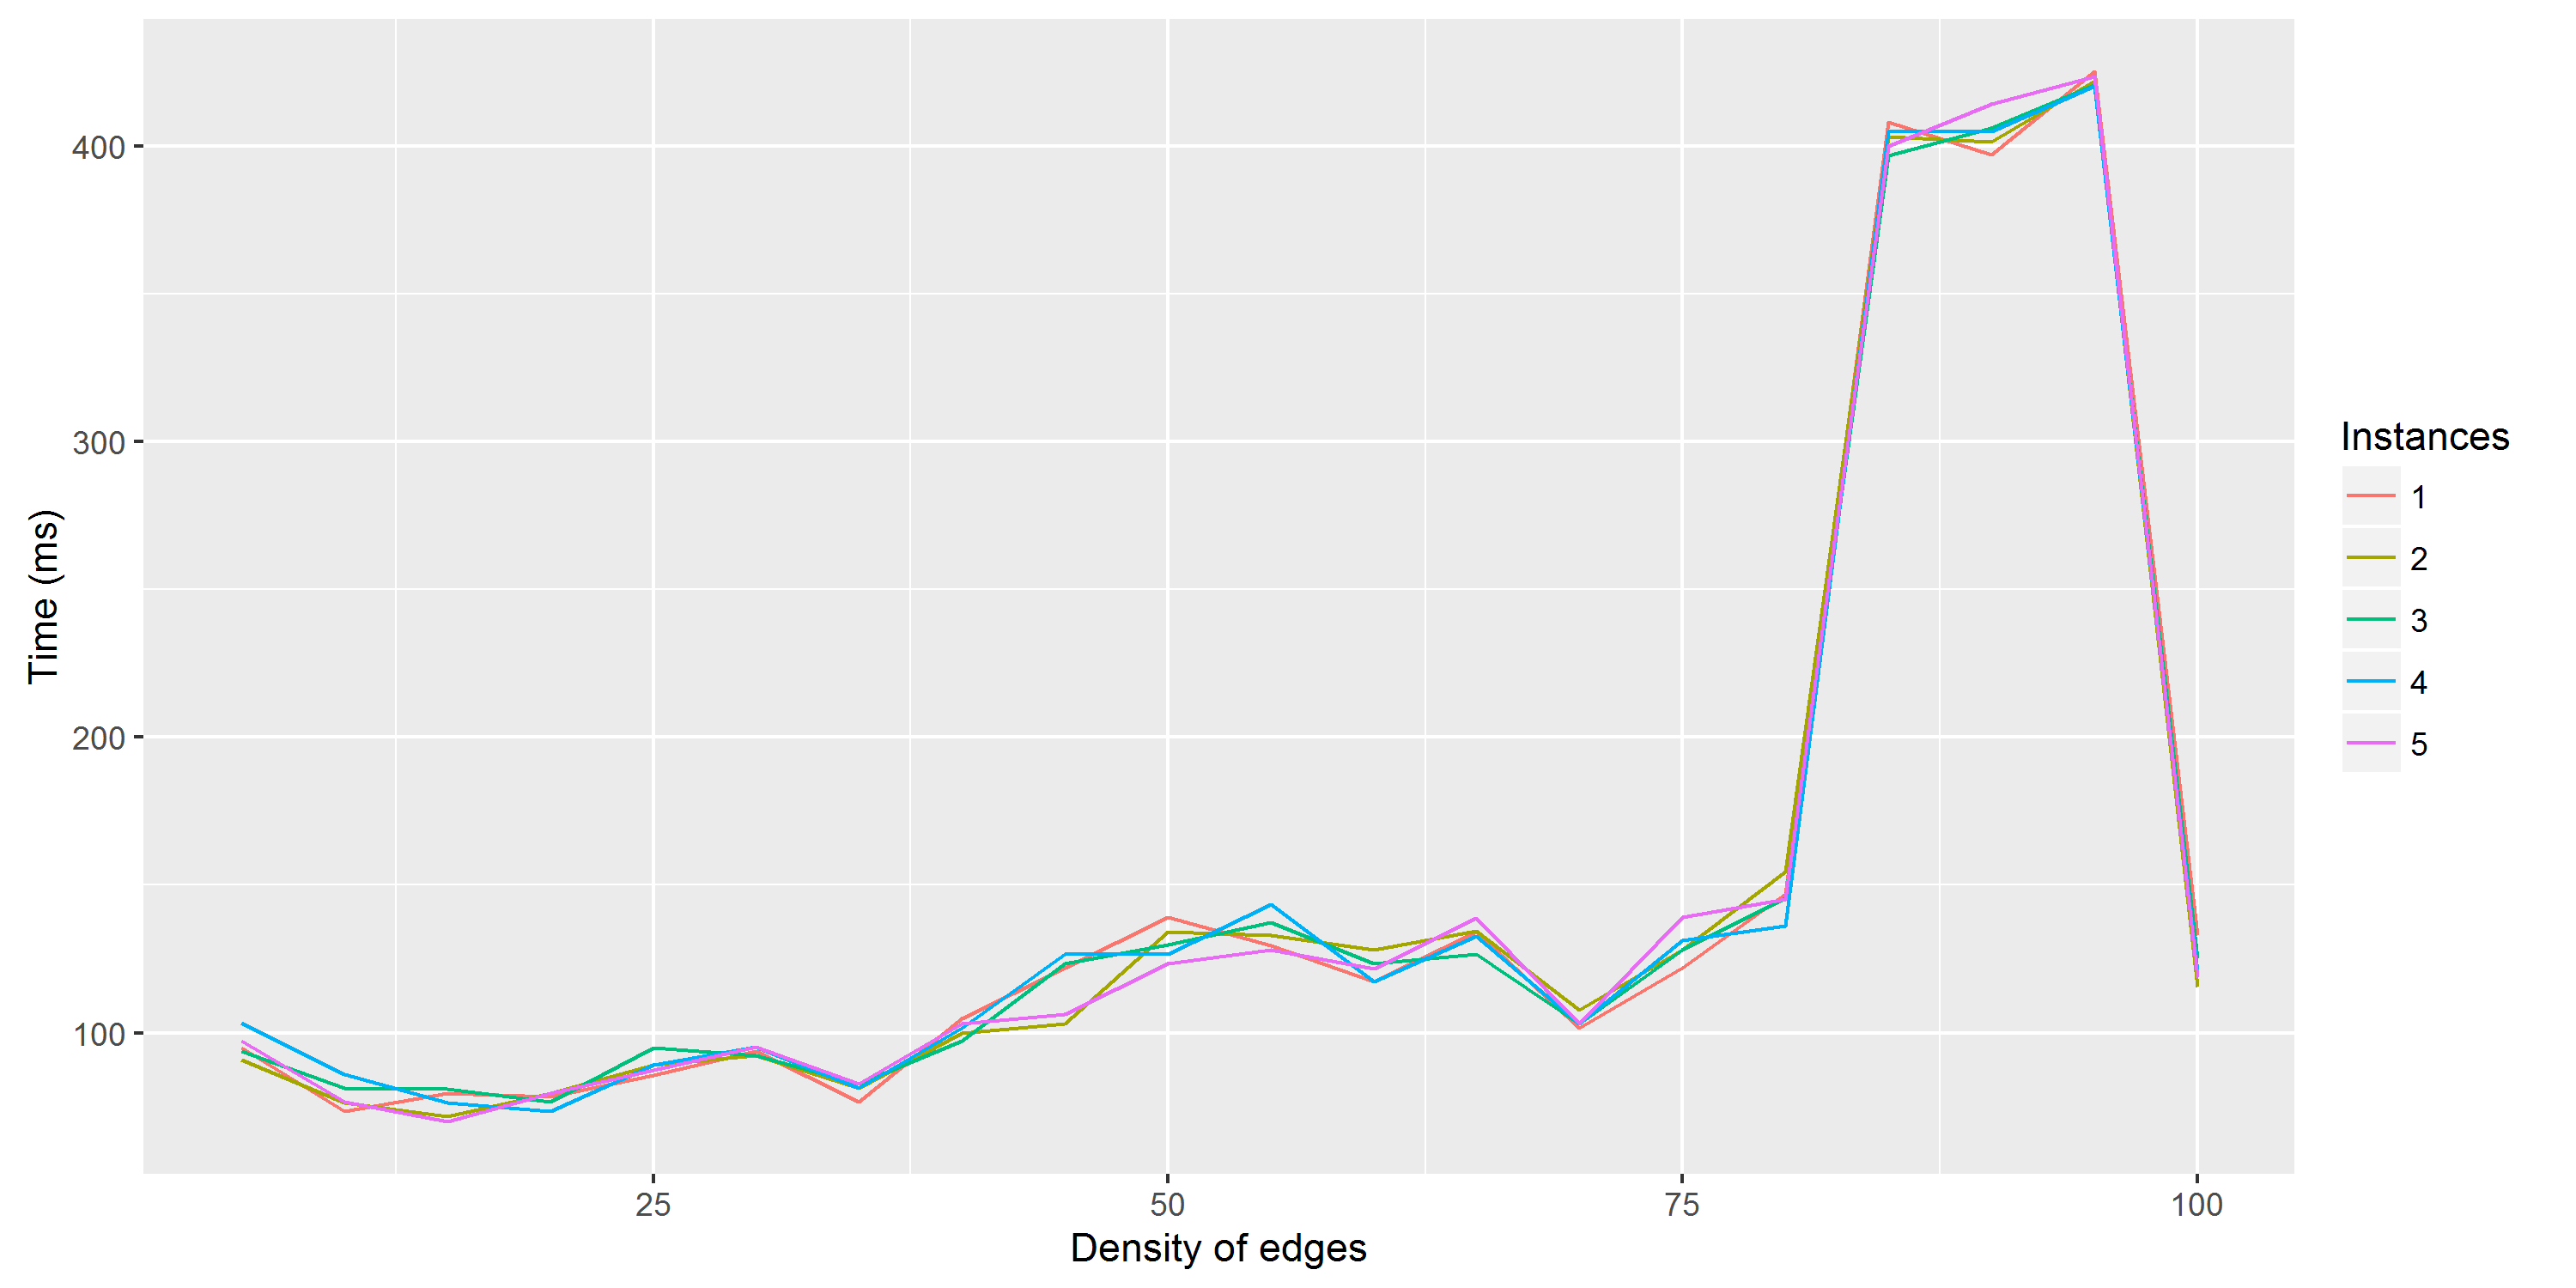
\includegraphics[scale=0.5]{images/results/ffmatching.png}
\caption{Run time of Ford-Fulkerson with scaling on all matching instances with the $sparse map$.}
\label{fig:ffmatching}
\end{center}
\end{figure}
\subsection{Push-Relabel}
\subsubsection{Density variation instances}
When we look at the results of the FIFO Push-Relabel, an observation is quite obvious : it is not regular at all. As shown in Figure~\ref{fig:PR6}, the run time on one density variation instance can vary from less than 100 ms to more than 5000 ms.
\begin{figure}[H]
\begin{center}
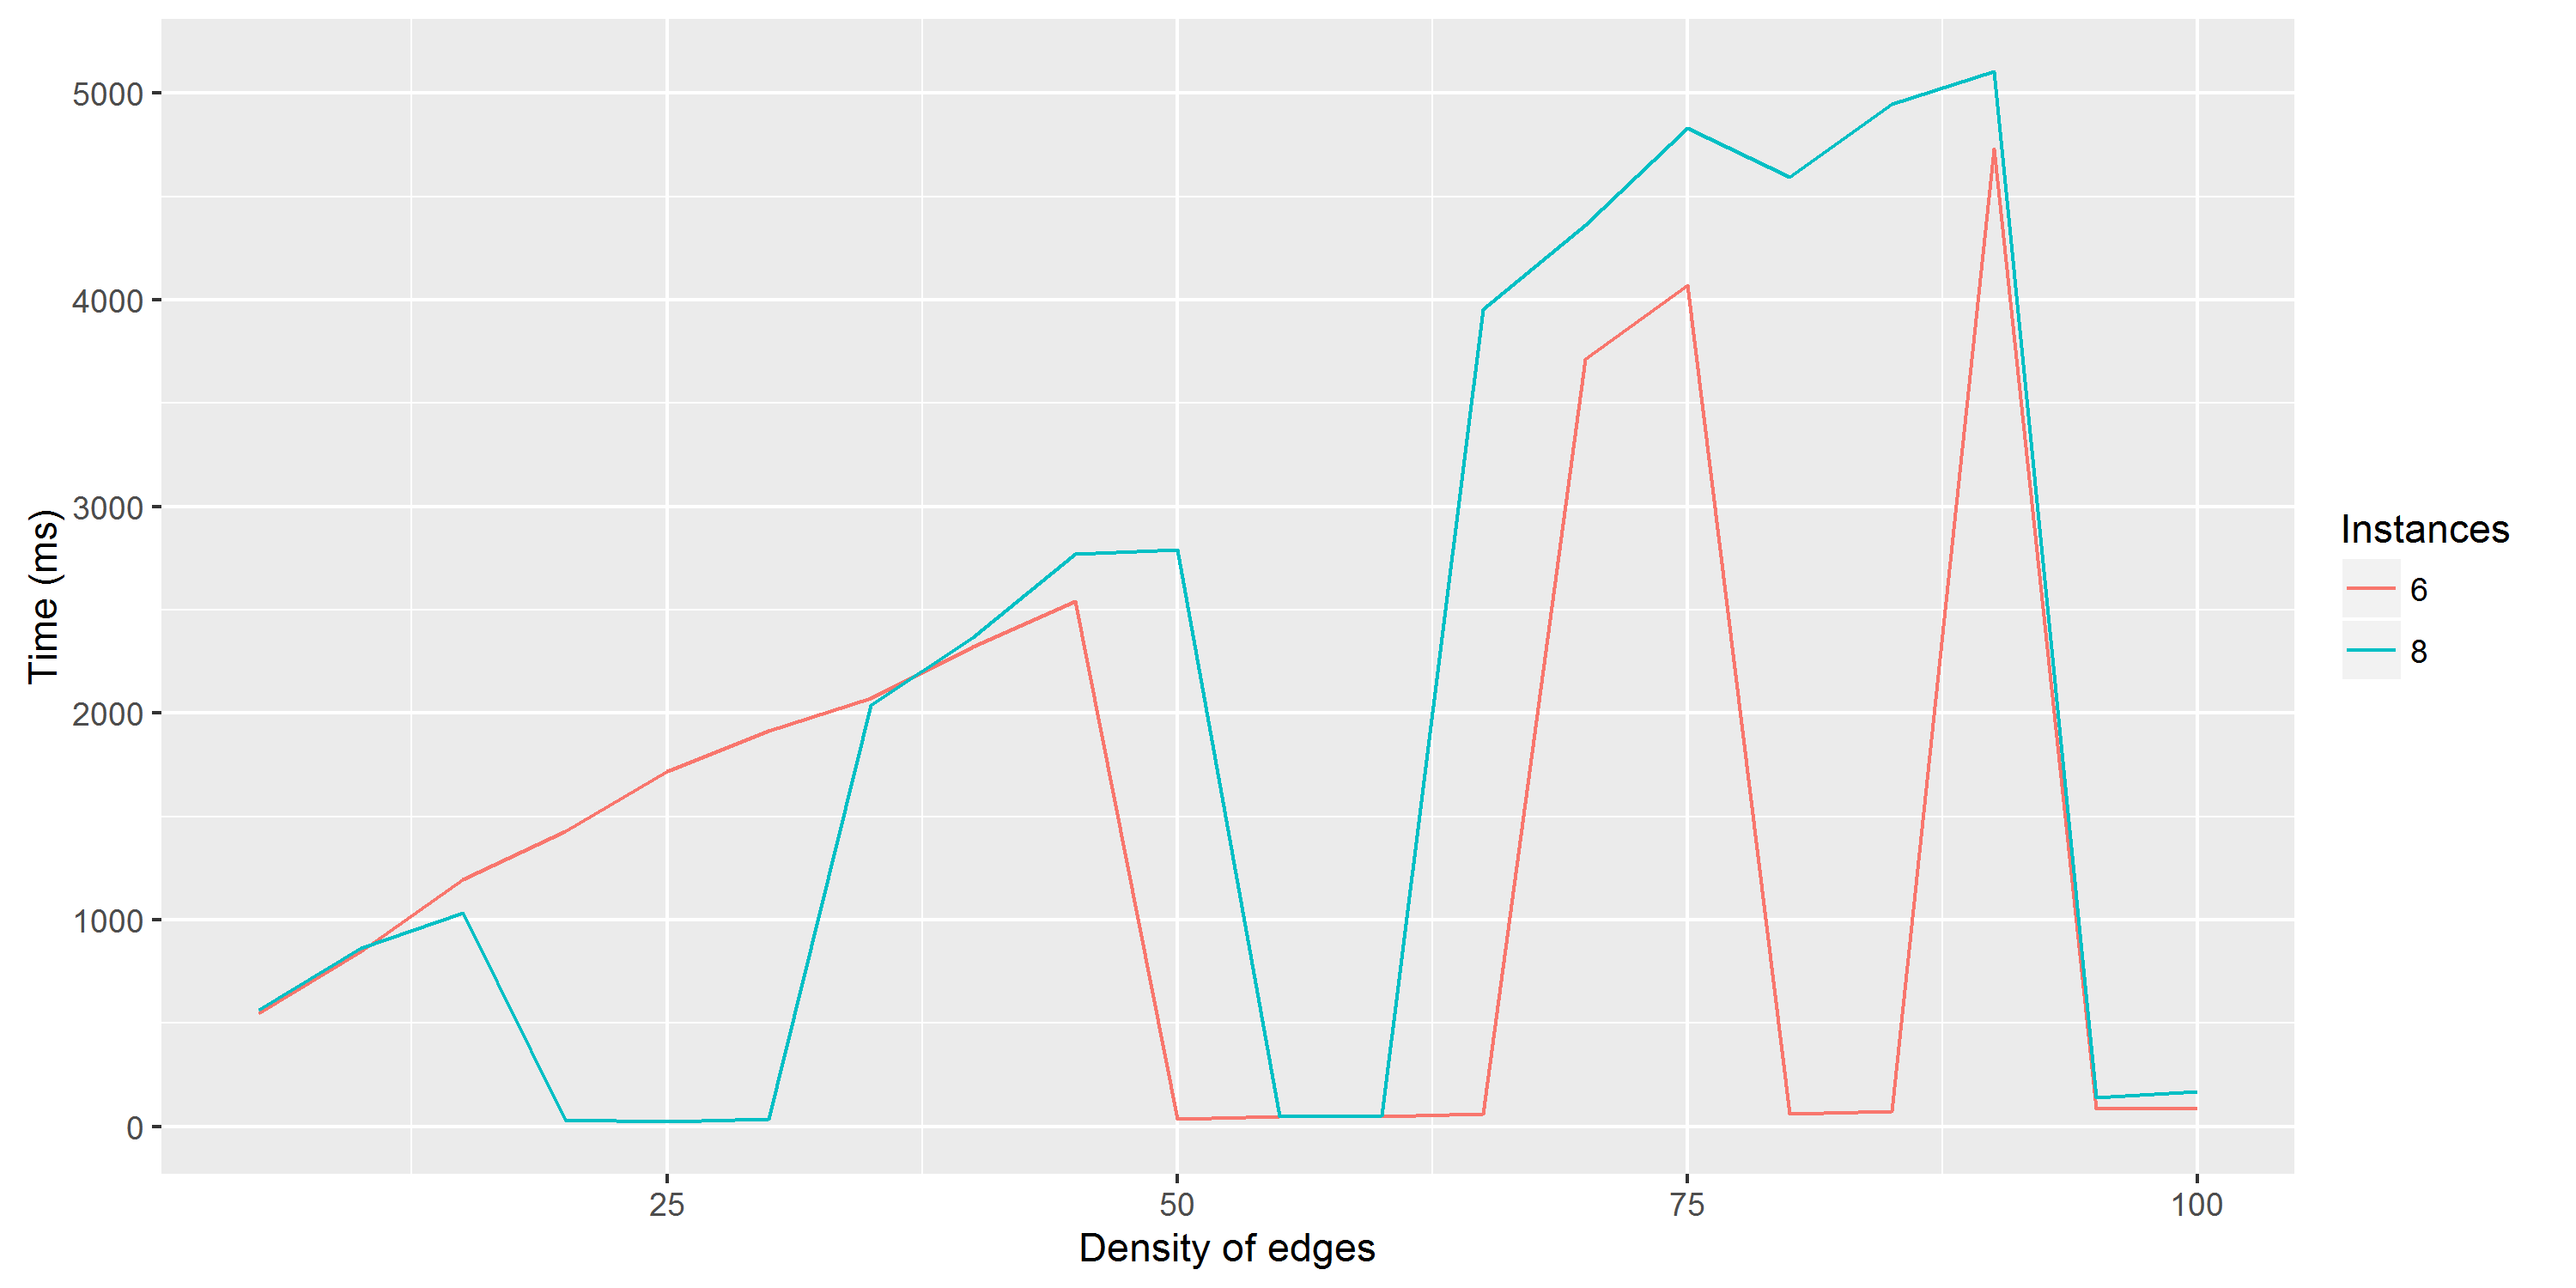
\includegraphics[scale=0.5]{images/results/pri68.png}
\caption{Run time of FIFO Push-Relabel on the density variation instance 6 and 8 with the $split array$.}
\label{fig:PR6}
\end{center}
\end{figure}
It may nevertheless have a stable run time but once very high and once extremely low. That is what we can observe in Figure~\ref{fig:PR10} and Figure~\ref{fig:PR7}.
\begin{figure}[H]
\begin{center}
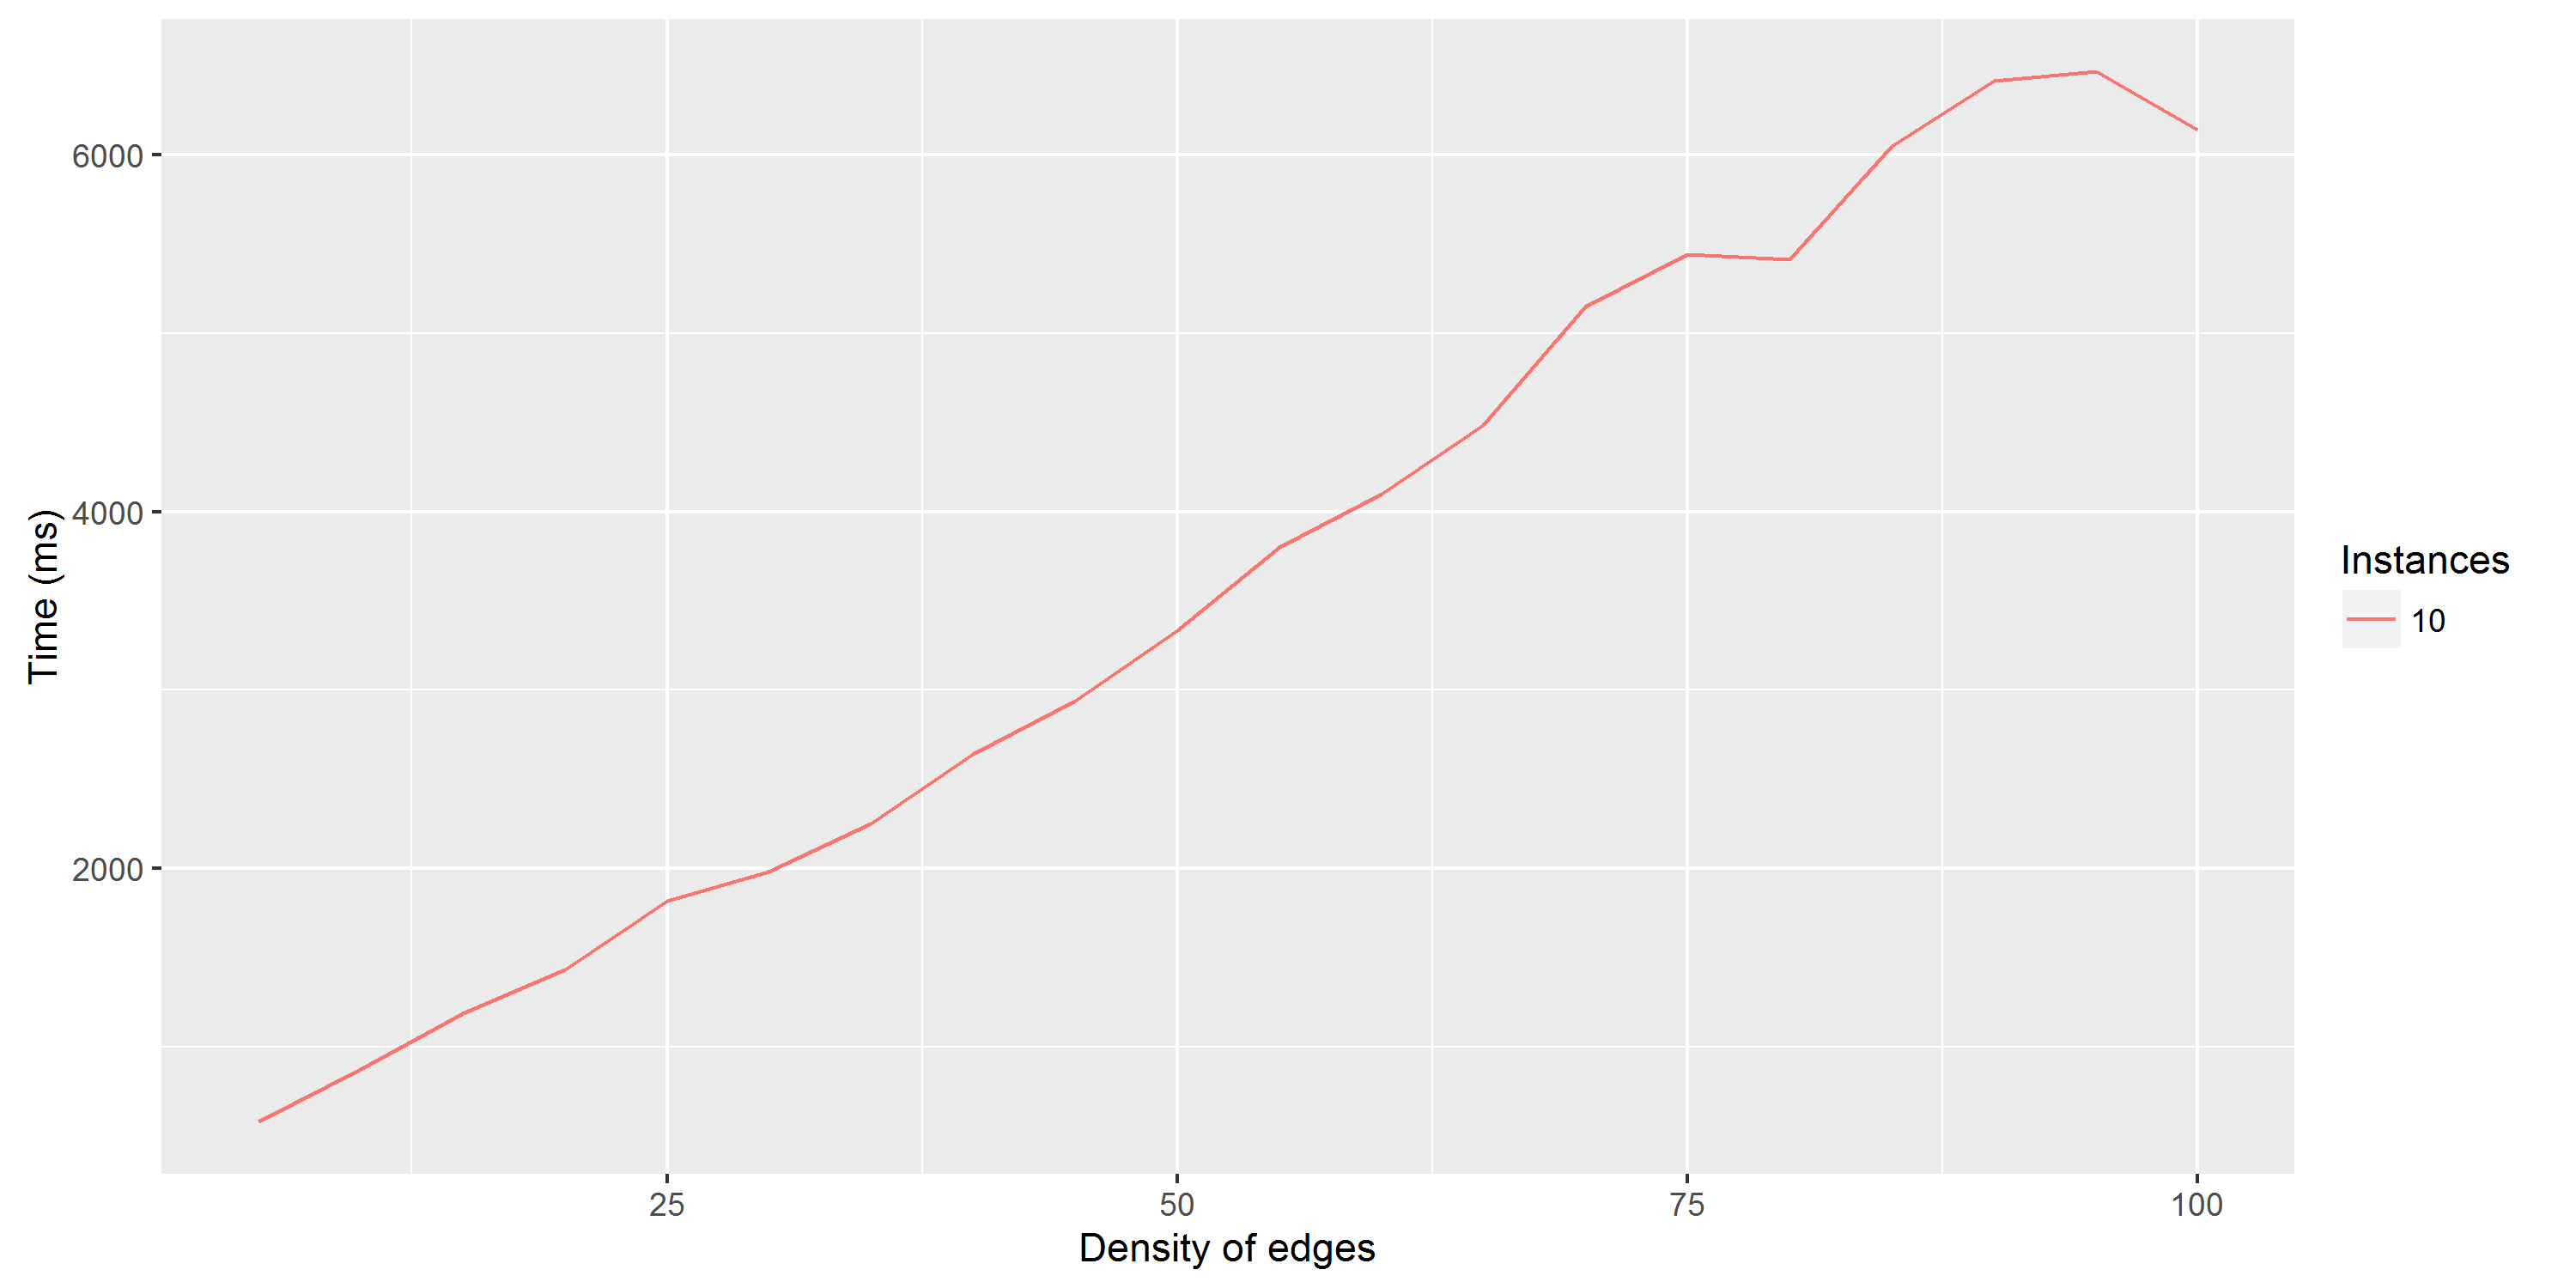
\includegraphics[scale=0.5]{images/results/pri10.png}
\caption{Run time of FIFO Push-Relabel on the density variation instance 10 with the $split array$.}
\label{fig:PR10}
\end{center}
\end{figure}
\begin{figure}[H]
\begin{center}
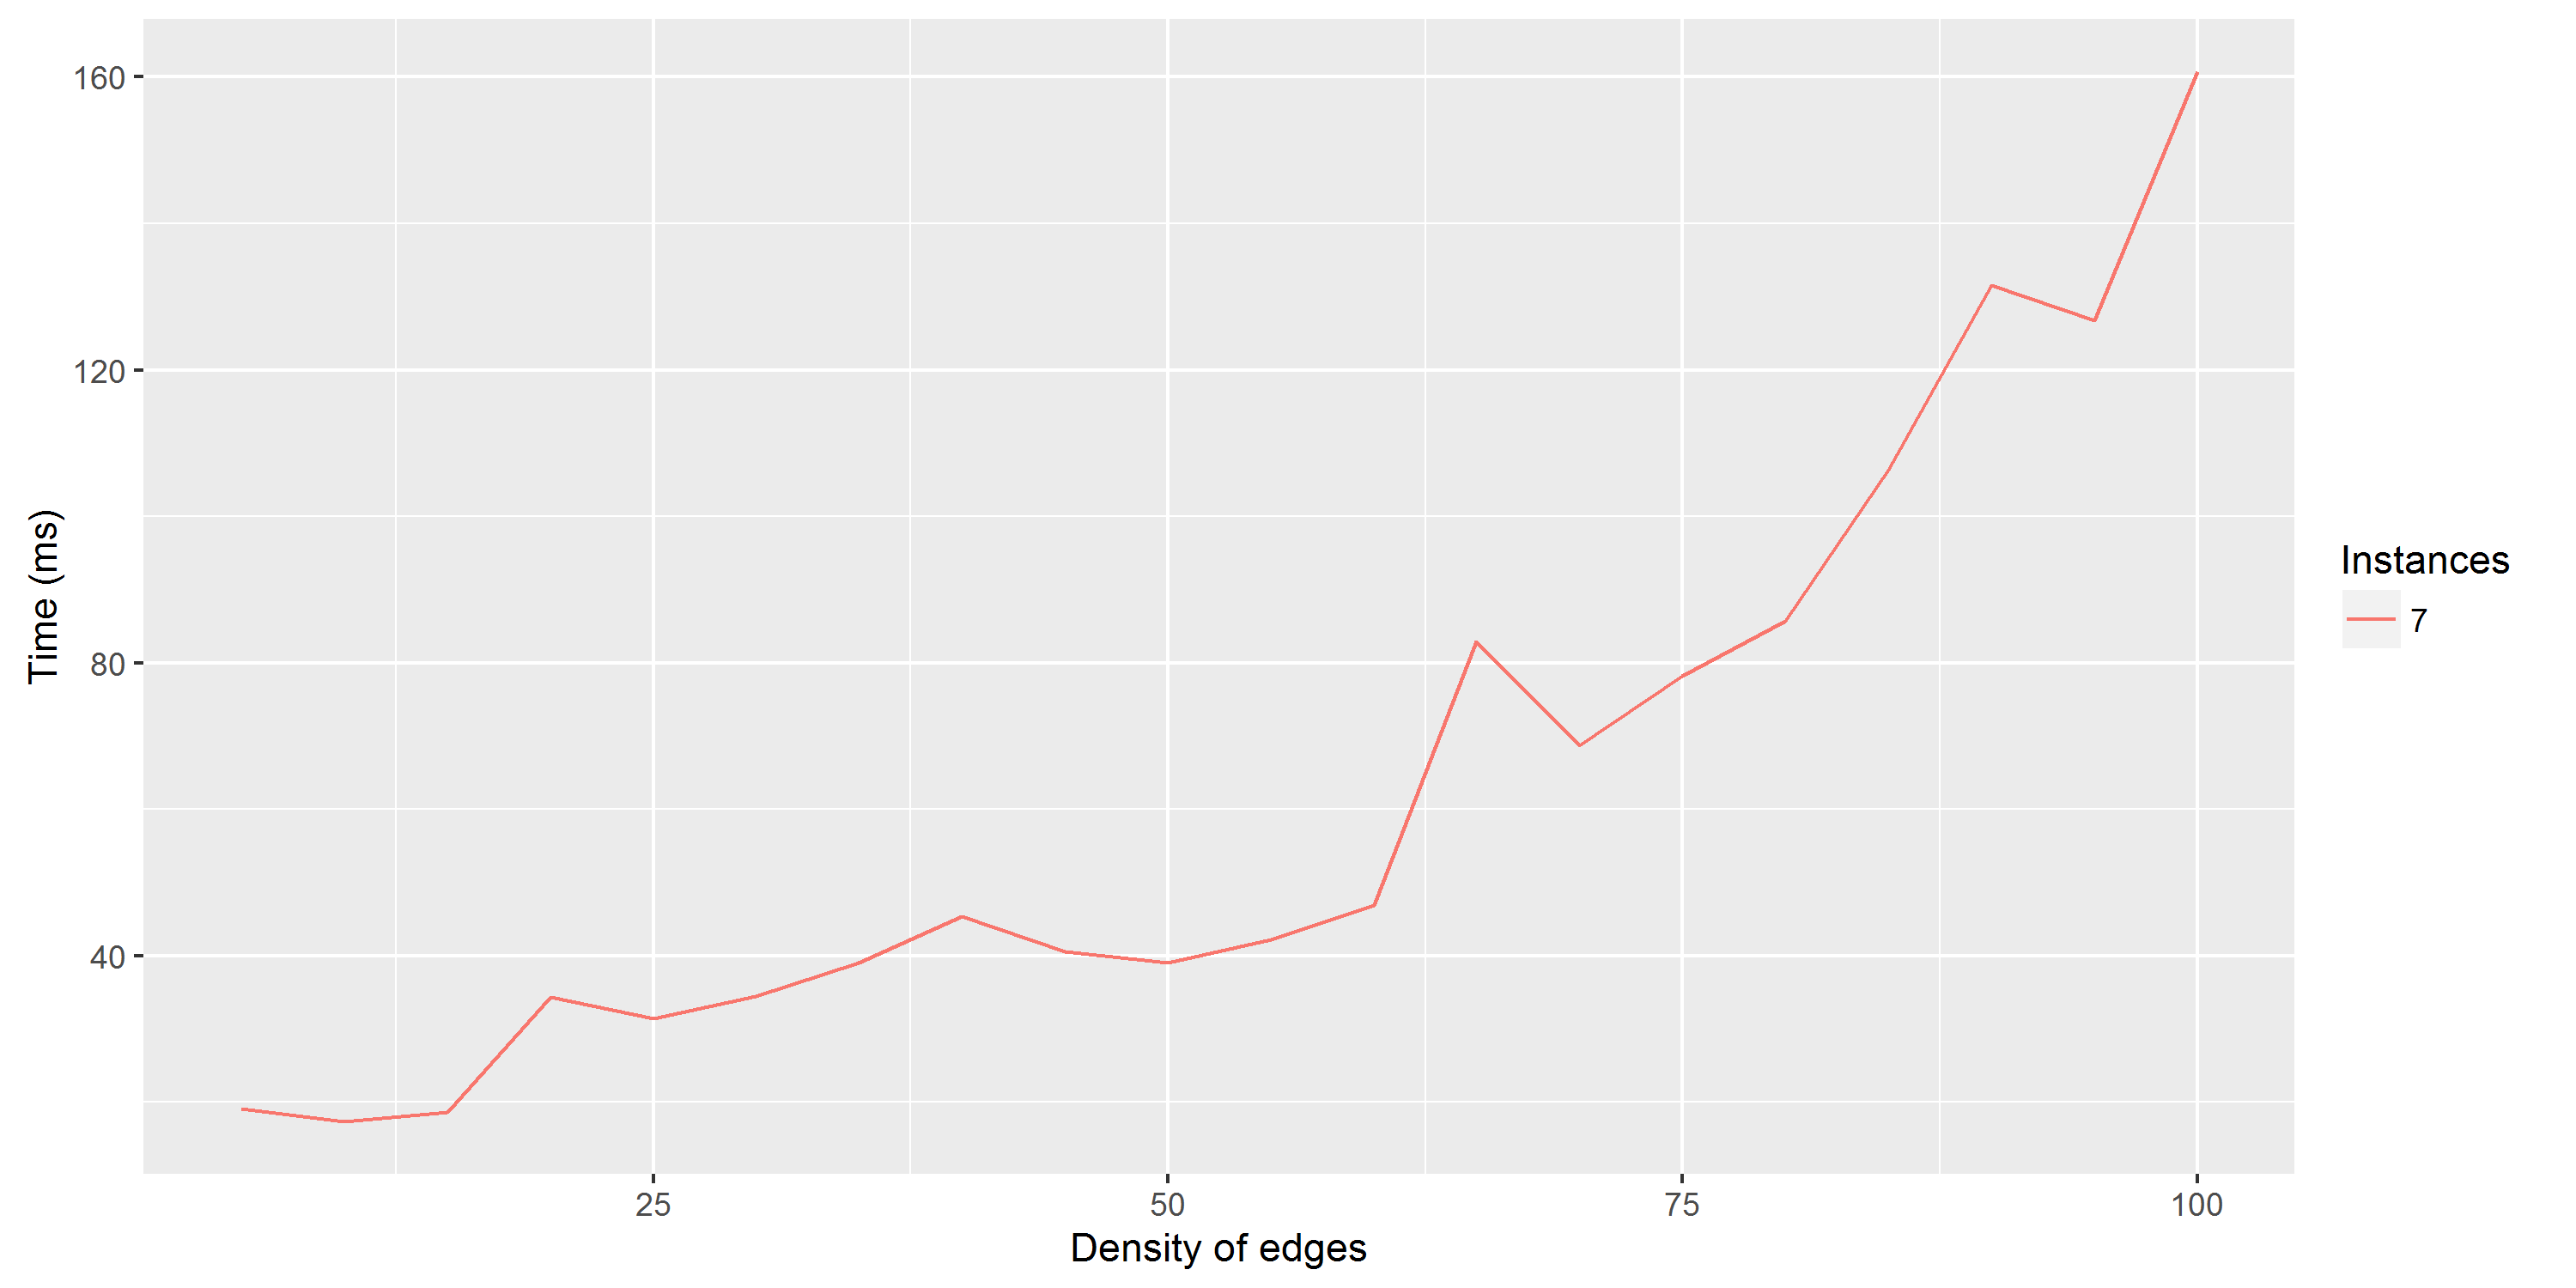
\includegraphics[scale=0.5]{images/results/pri7.png}
\caption{Run time of FIFO Push-Relabel on the density variation instance 7 with the $split array$.}
\label{fig:PR7}
\end{center}
\end{figure}
When displaying the run time of each density variation instance with its best data structure, we obtain a very disparate graph, as we can see in Figure~\ref{fig:PRmean}. Indeed, the FIFO Push-Relabel solve the maximum flow problem on complete graphs with $|V|=1000$ with a run time ranging from 100 ms to 6700 ms.
\begin{figure}[H]
\begin{center}
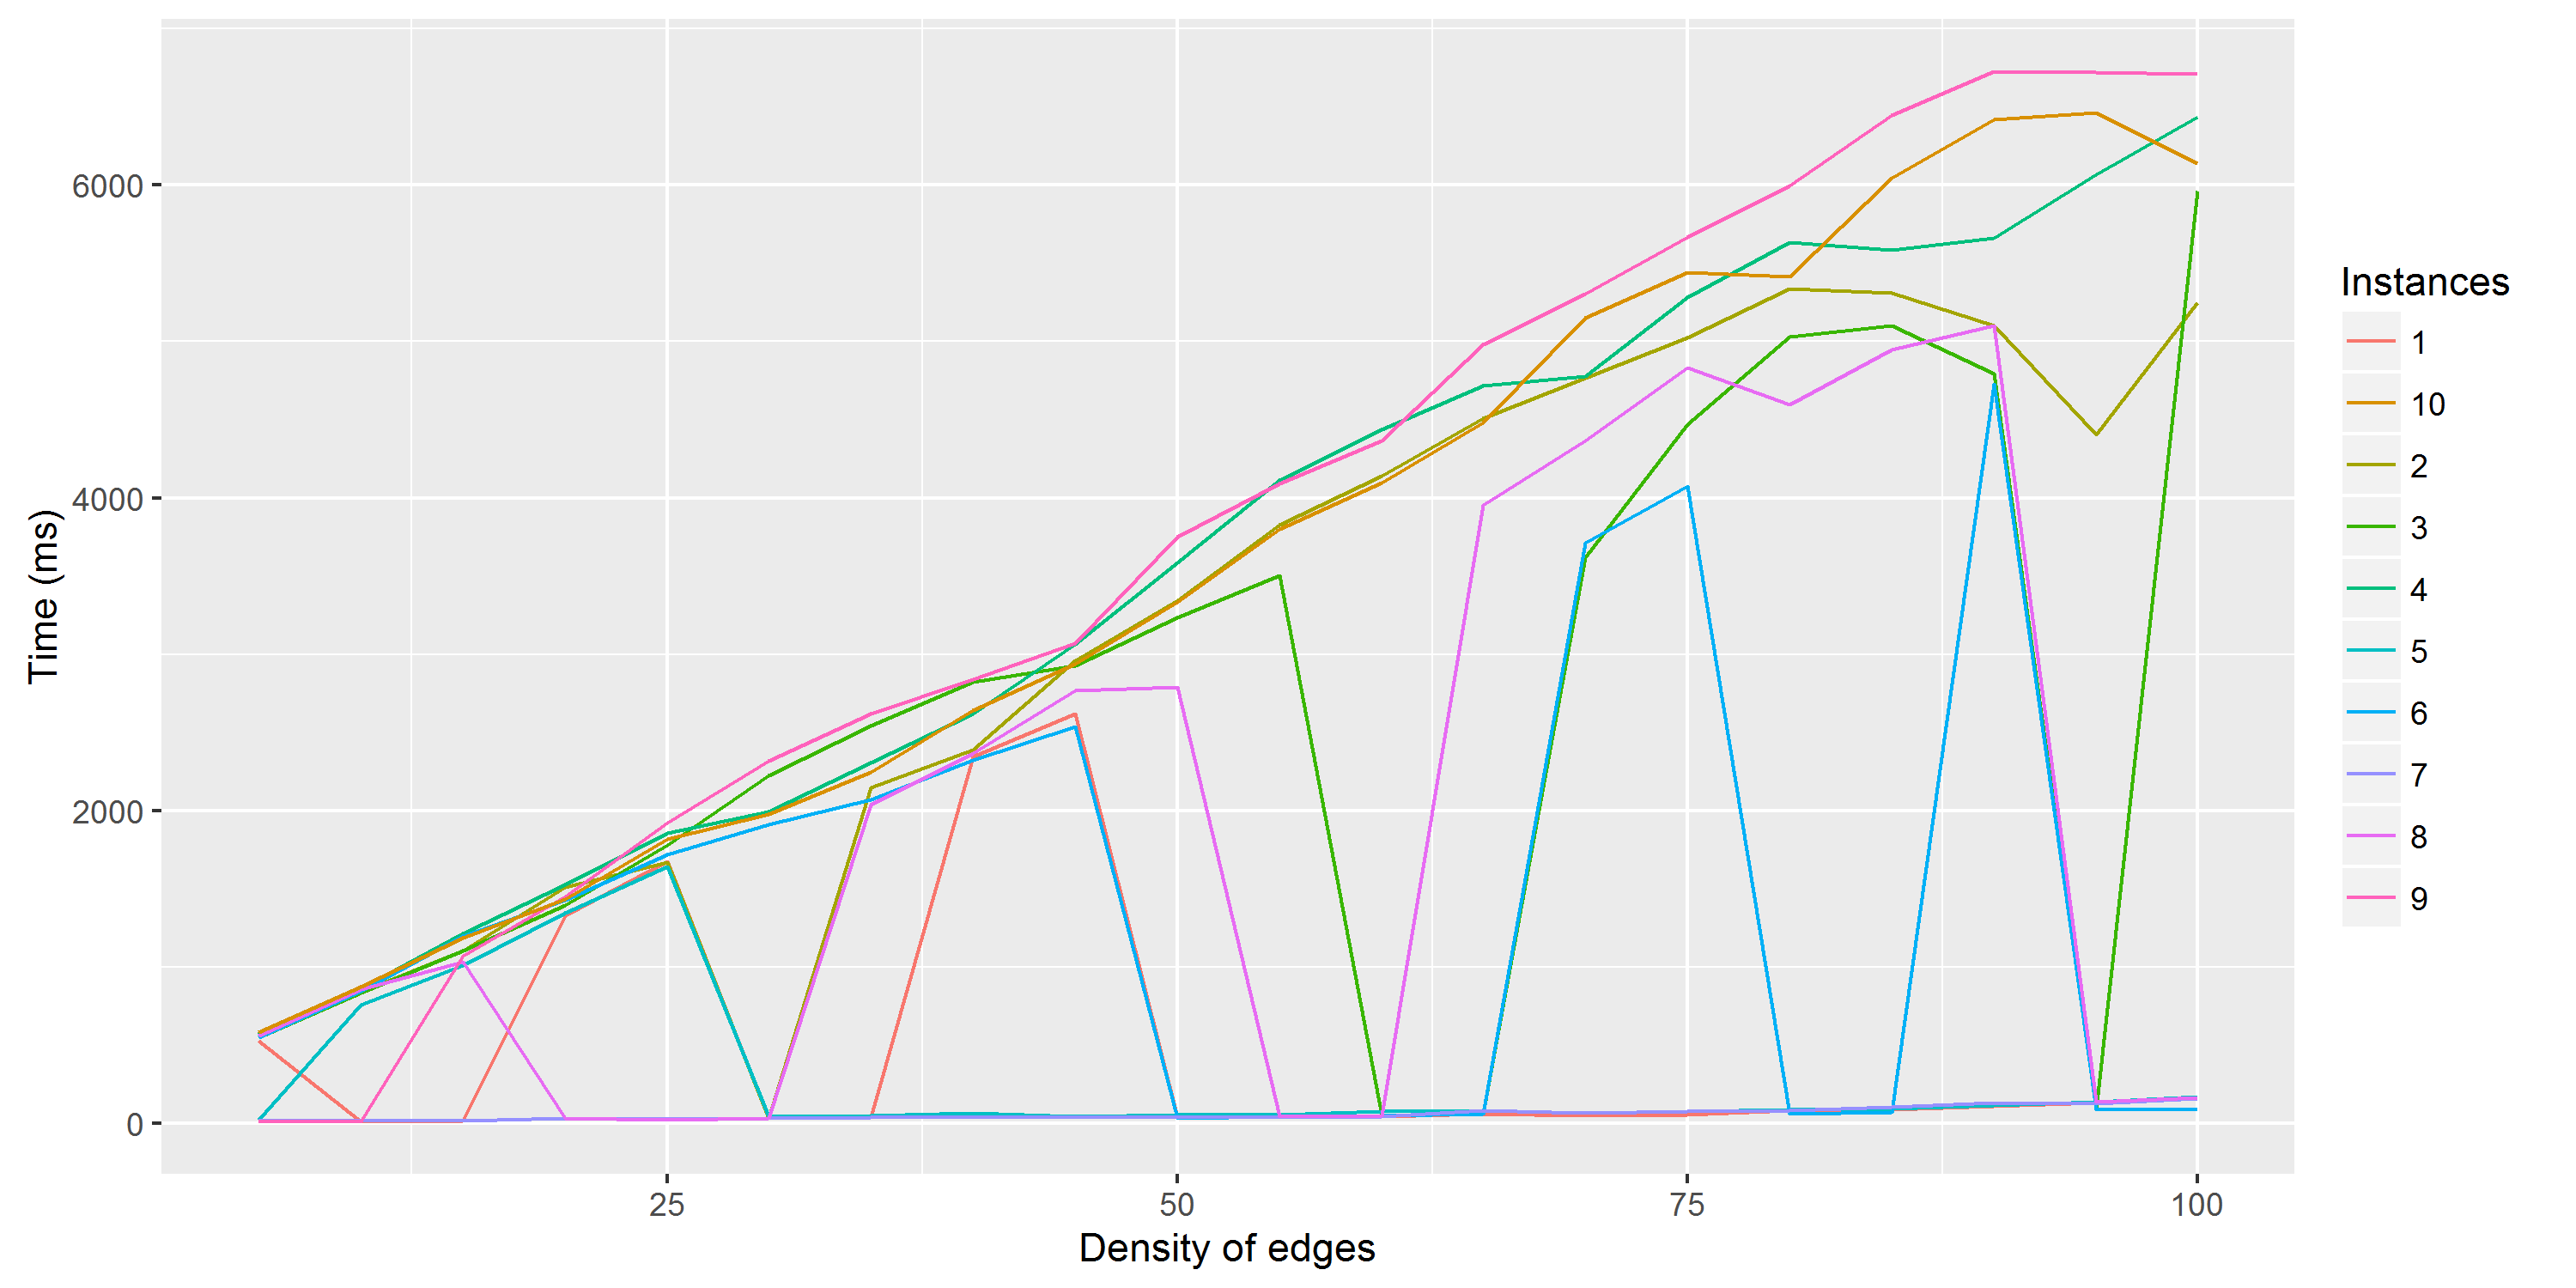
\includegraphics[scale=0.5]{images/results/PRmean.png}
\caption{Run time of FIFO Push-Relabel on all density variation instances with the $split array$.}
\label{fig:PRmean}
\end{center}
\end{figure}
\subsubsection{Size variation instances}
Contrary to the results obtained on the density variation instances, the Highest Label Push-Relabel is regular but it offers catastrophic performances. Indeed, it has a run time ranging from 85000 to 125000 ms to solve the maximum flow problem on graphs with $|V|=5000$ and a density of edges equal to 10\%. It is 1000 times slower than Edmonds-Karp.
\begin{figure}[H]
\begin{center}
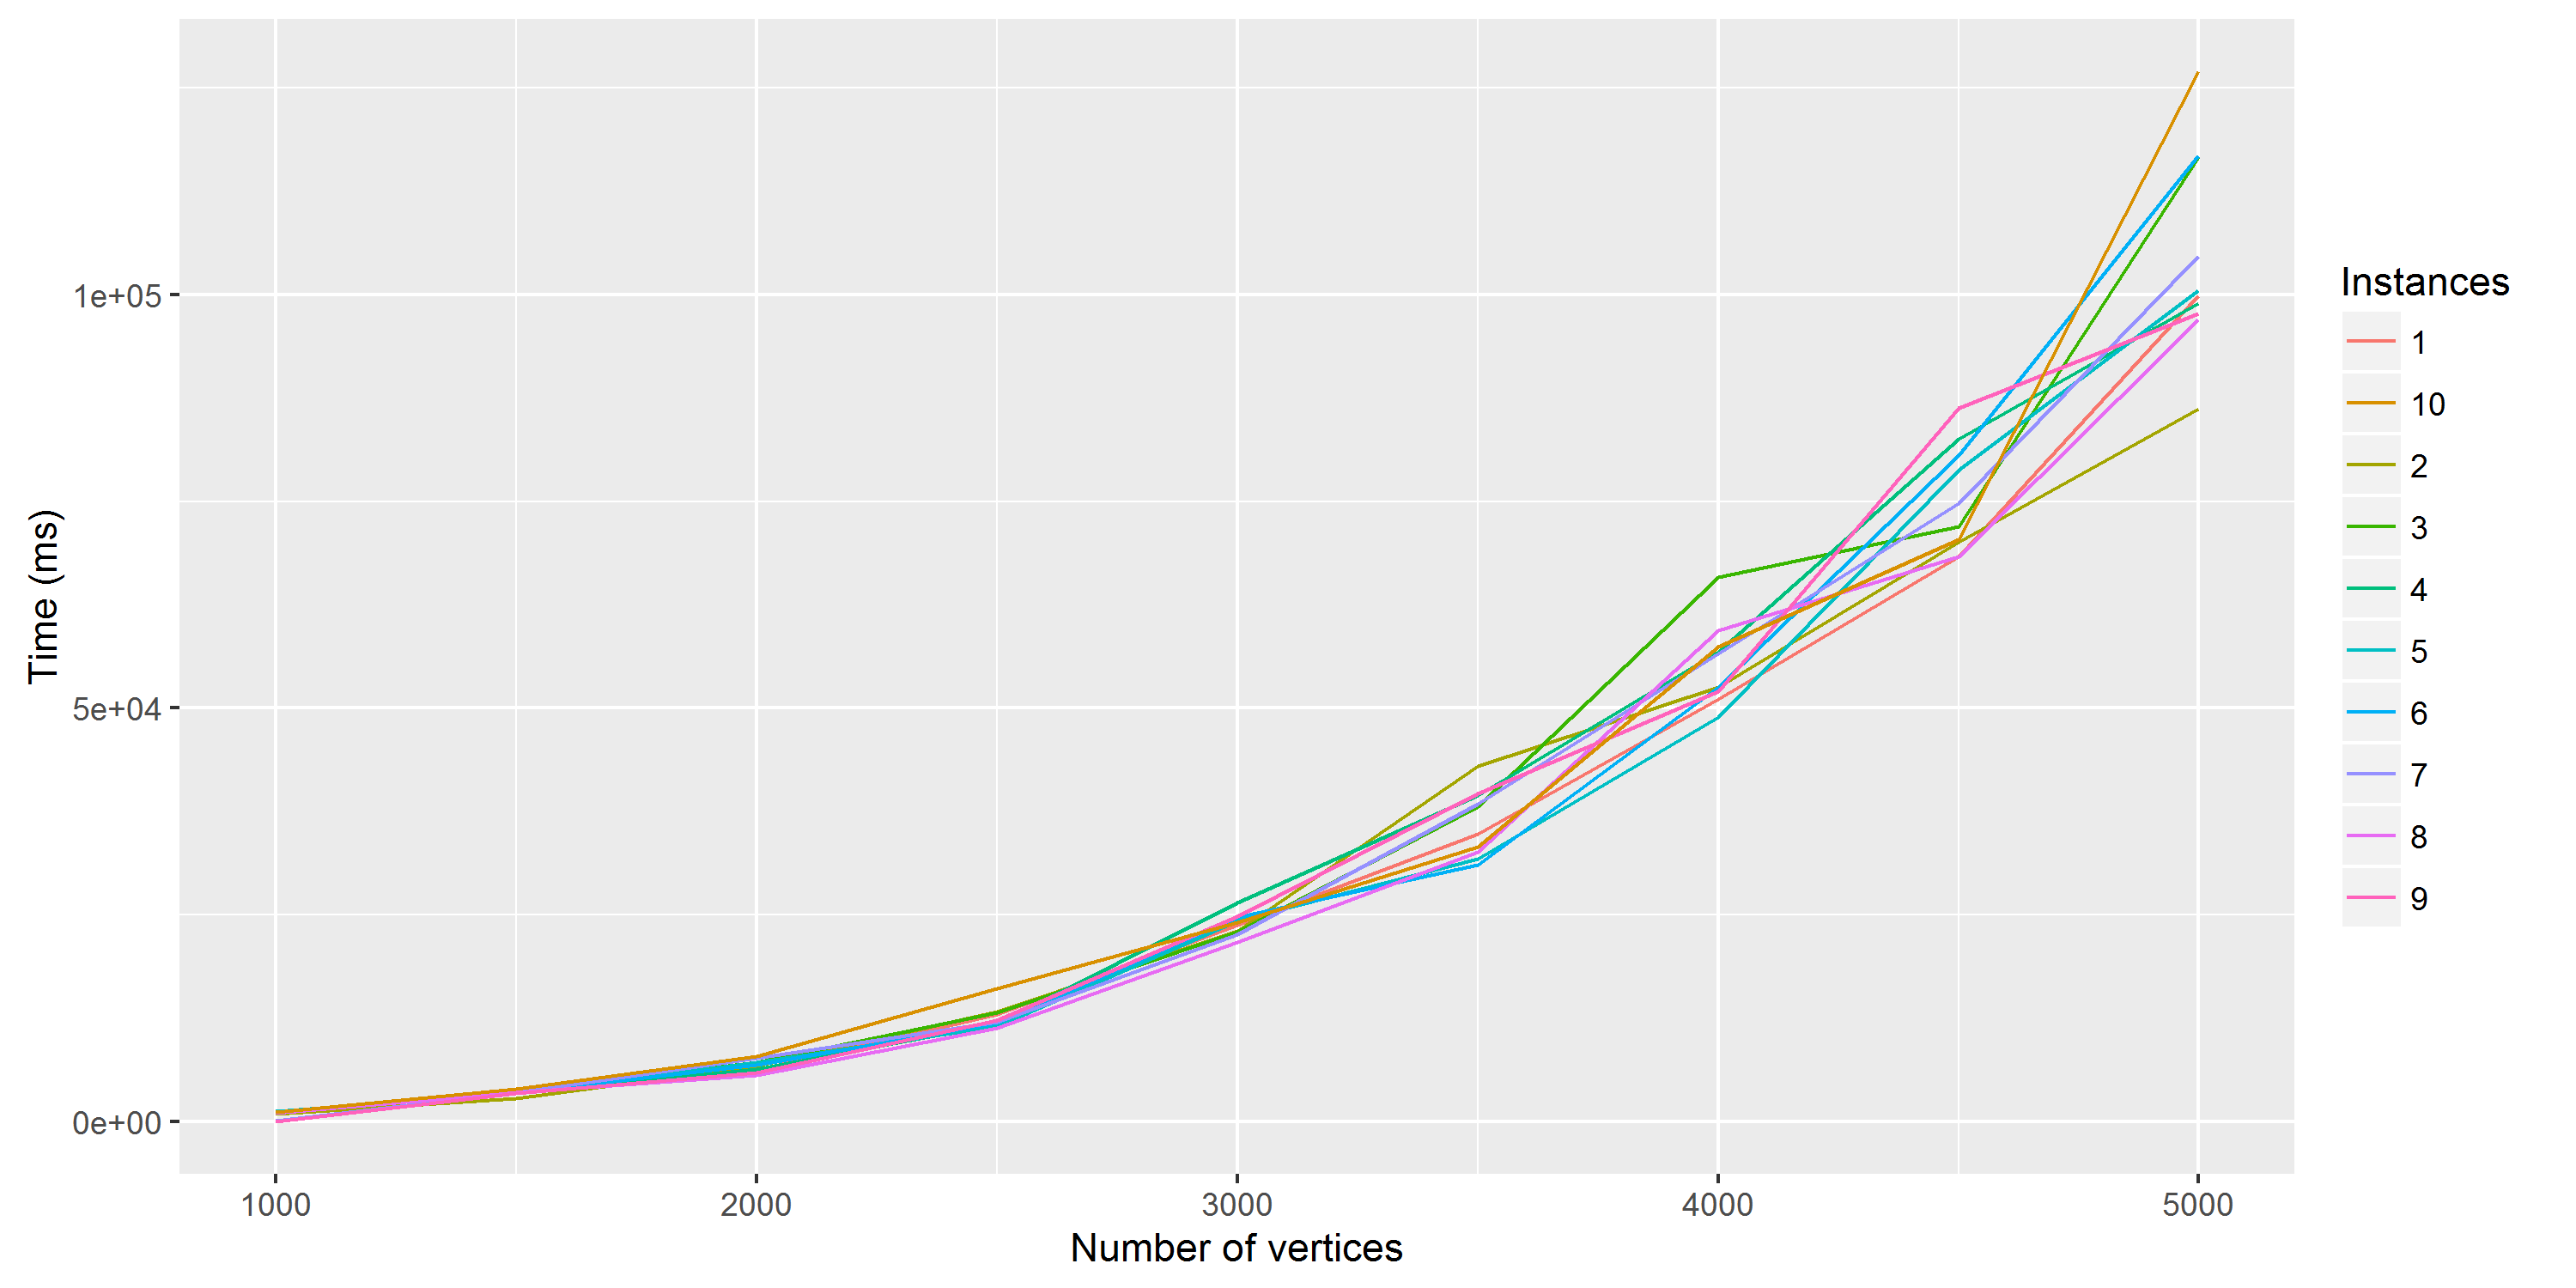
\includegraphics[scale=0.5]{images/results/HLPRmean.png}
\caption{Run time of Highest Label Push-Relabel on all size variation instances with the $split array$.}
\label{fig:HLPRmean}
\end{center}
\end{figure}
\subsubsection{Matching instances}
The Highest Label Push-Relabel excels in this type of instances. Indeed, it has a regular run time ranging from 20 to 30 ms to solve a matching instance with a maximum density of edges.
\begin{figure}[H]
\begin{center}
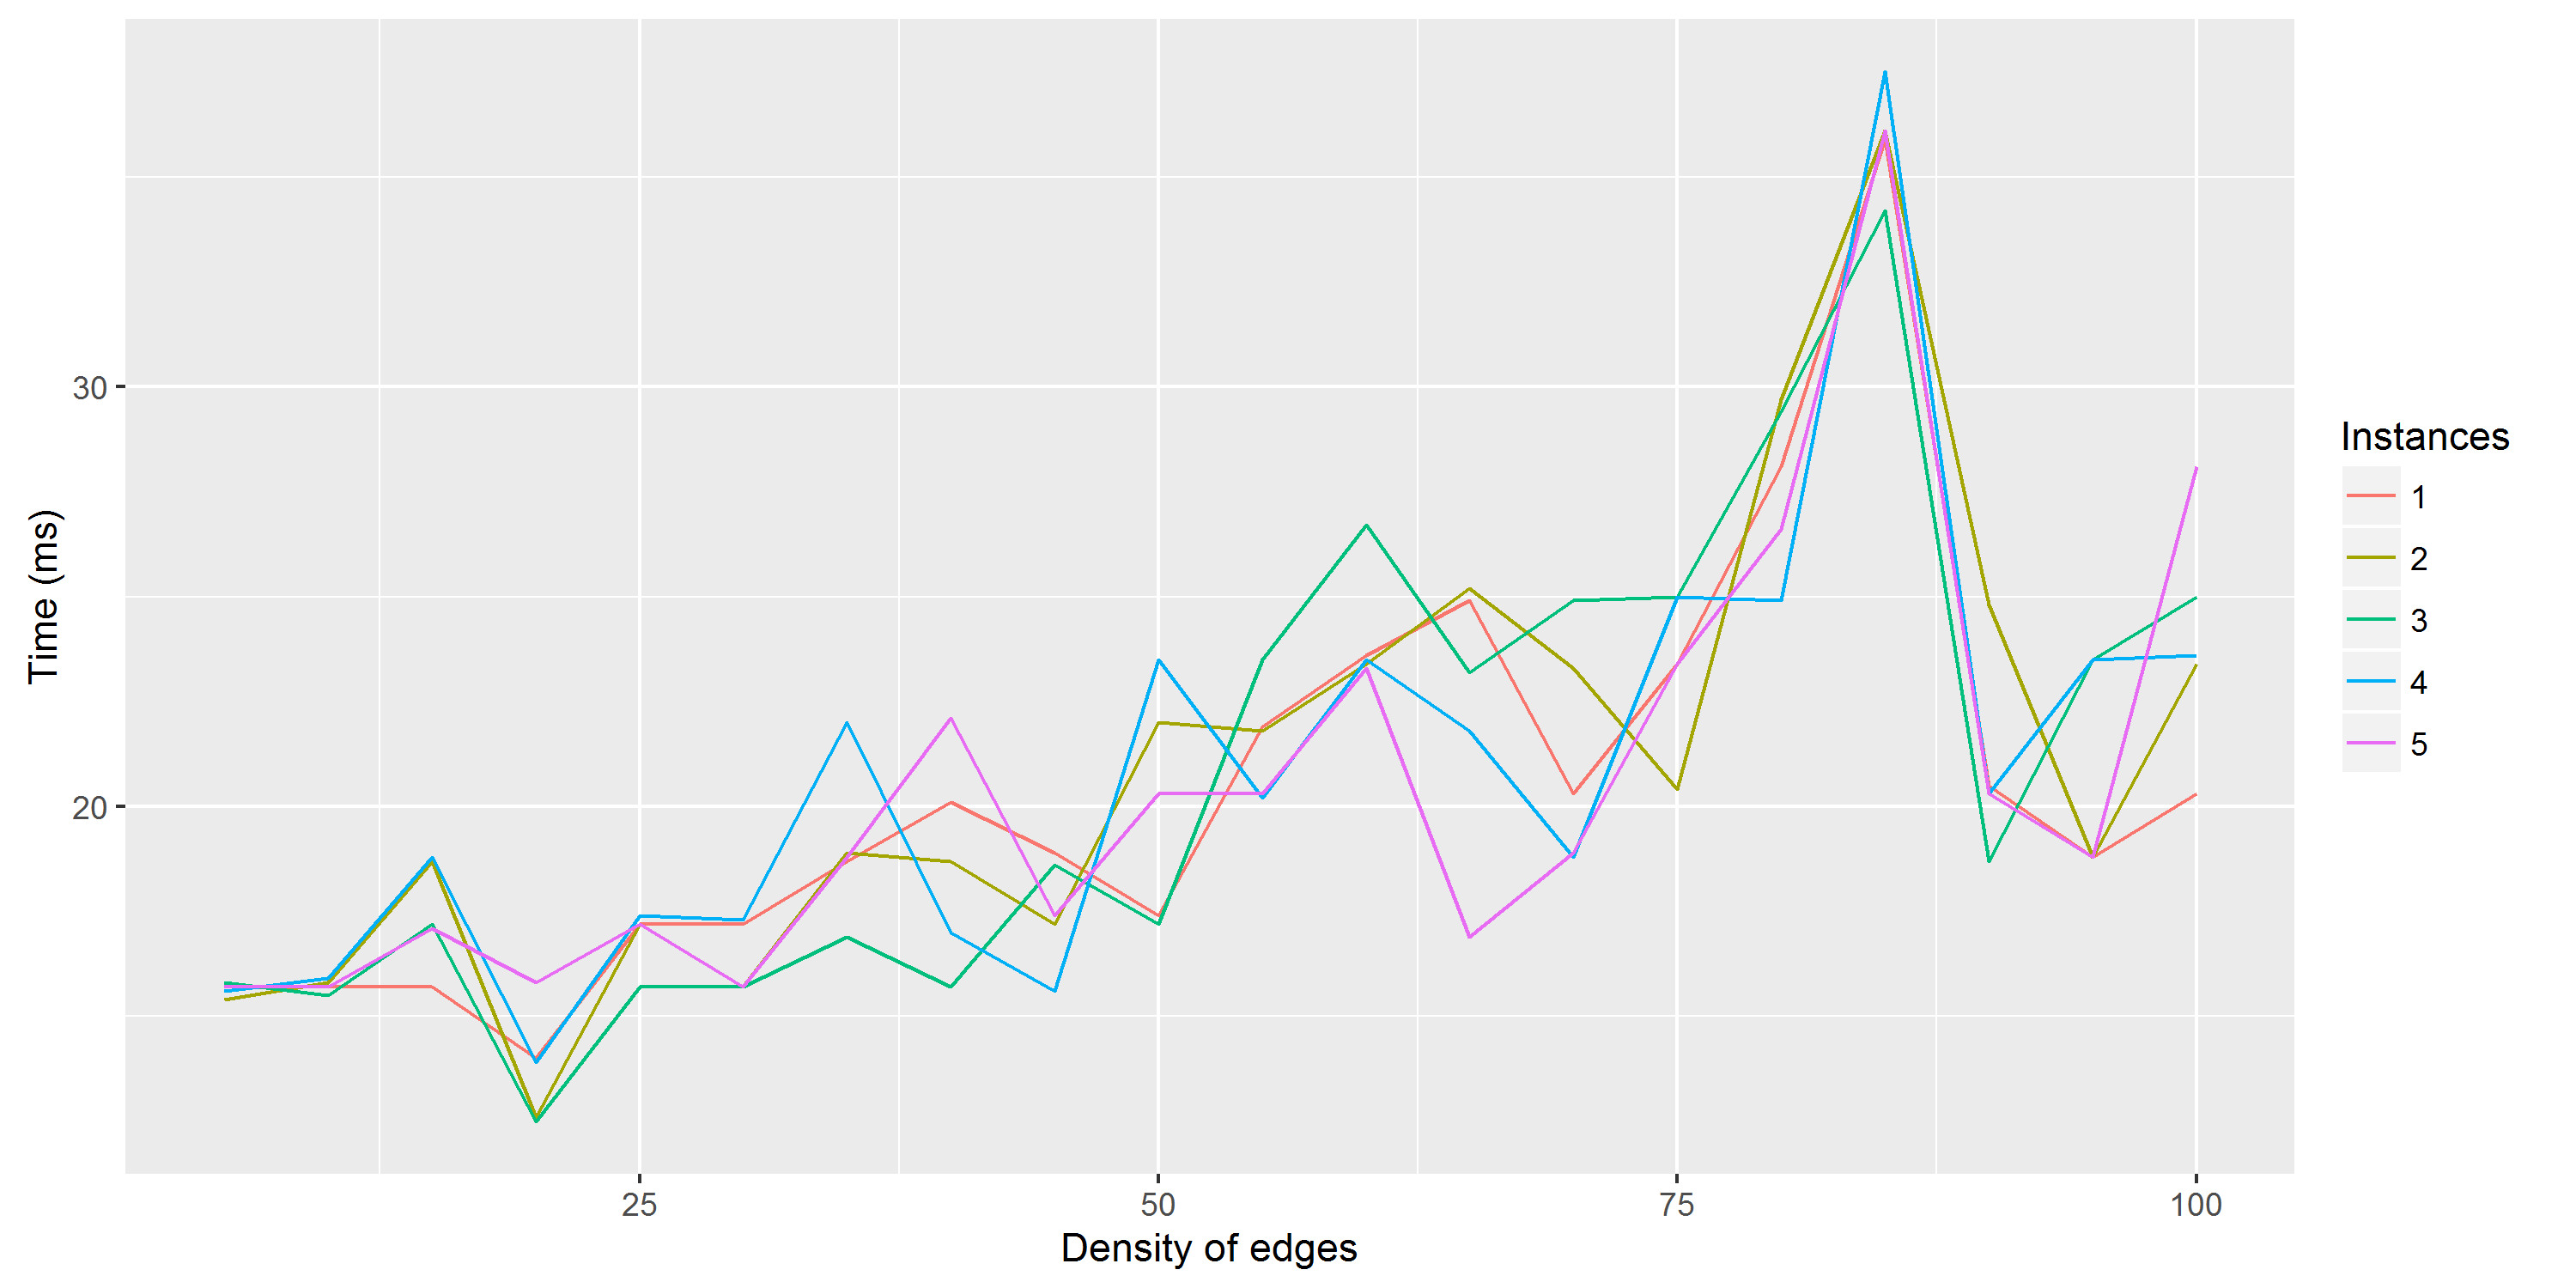
\includegraphics[scale=0.5]{images/results/prmatching.png}
\caption{Run time of Highest Label Push-Relabel on all matching instances with the $split array$.}
\label{fig:prmatching}
\end{center}
\end{figure}
\section{Comparison}
